\section{Spectrum Estimation}

\subsection{Discrete Fourier Transform Basics}

\noindent{}a. The ideal Fourier (magnitude) spectrum of a 20 Hz sine wave and the theoretical continuous frequency DTFT (magnitude) spectrum for a windowed sine wave at 20 Hz are shown below. Since a sine wave is a real periodic signal, we expect the ideal magnitude spectrum to be an even function consisting of only dirac delta functions. The magnitude spectrum of the rectangular window used is a sinc function. The ideal magnitude spectrum is convoluted with the sinc function to produce the theoretical continuous frequency DTFT (magnitude) spectrum. 

\begin{figure}[H]
\centering{}
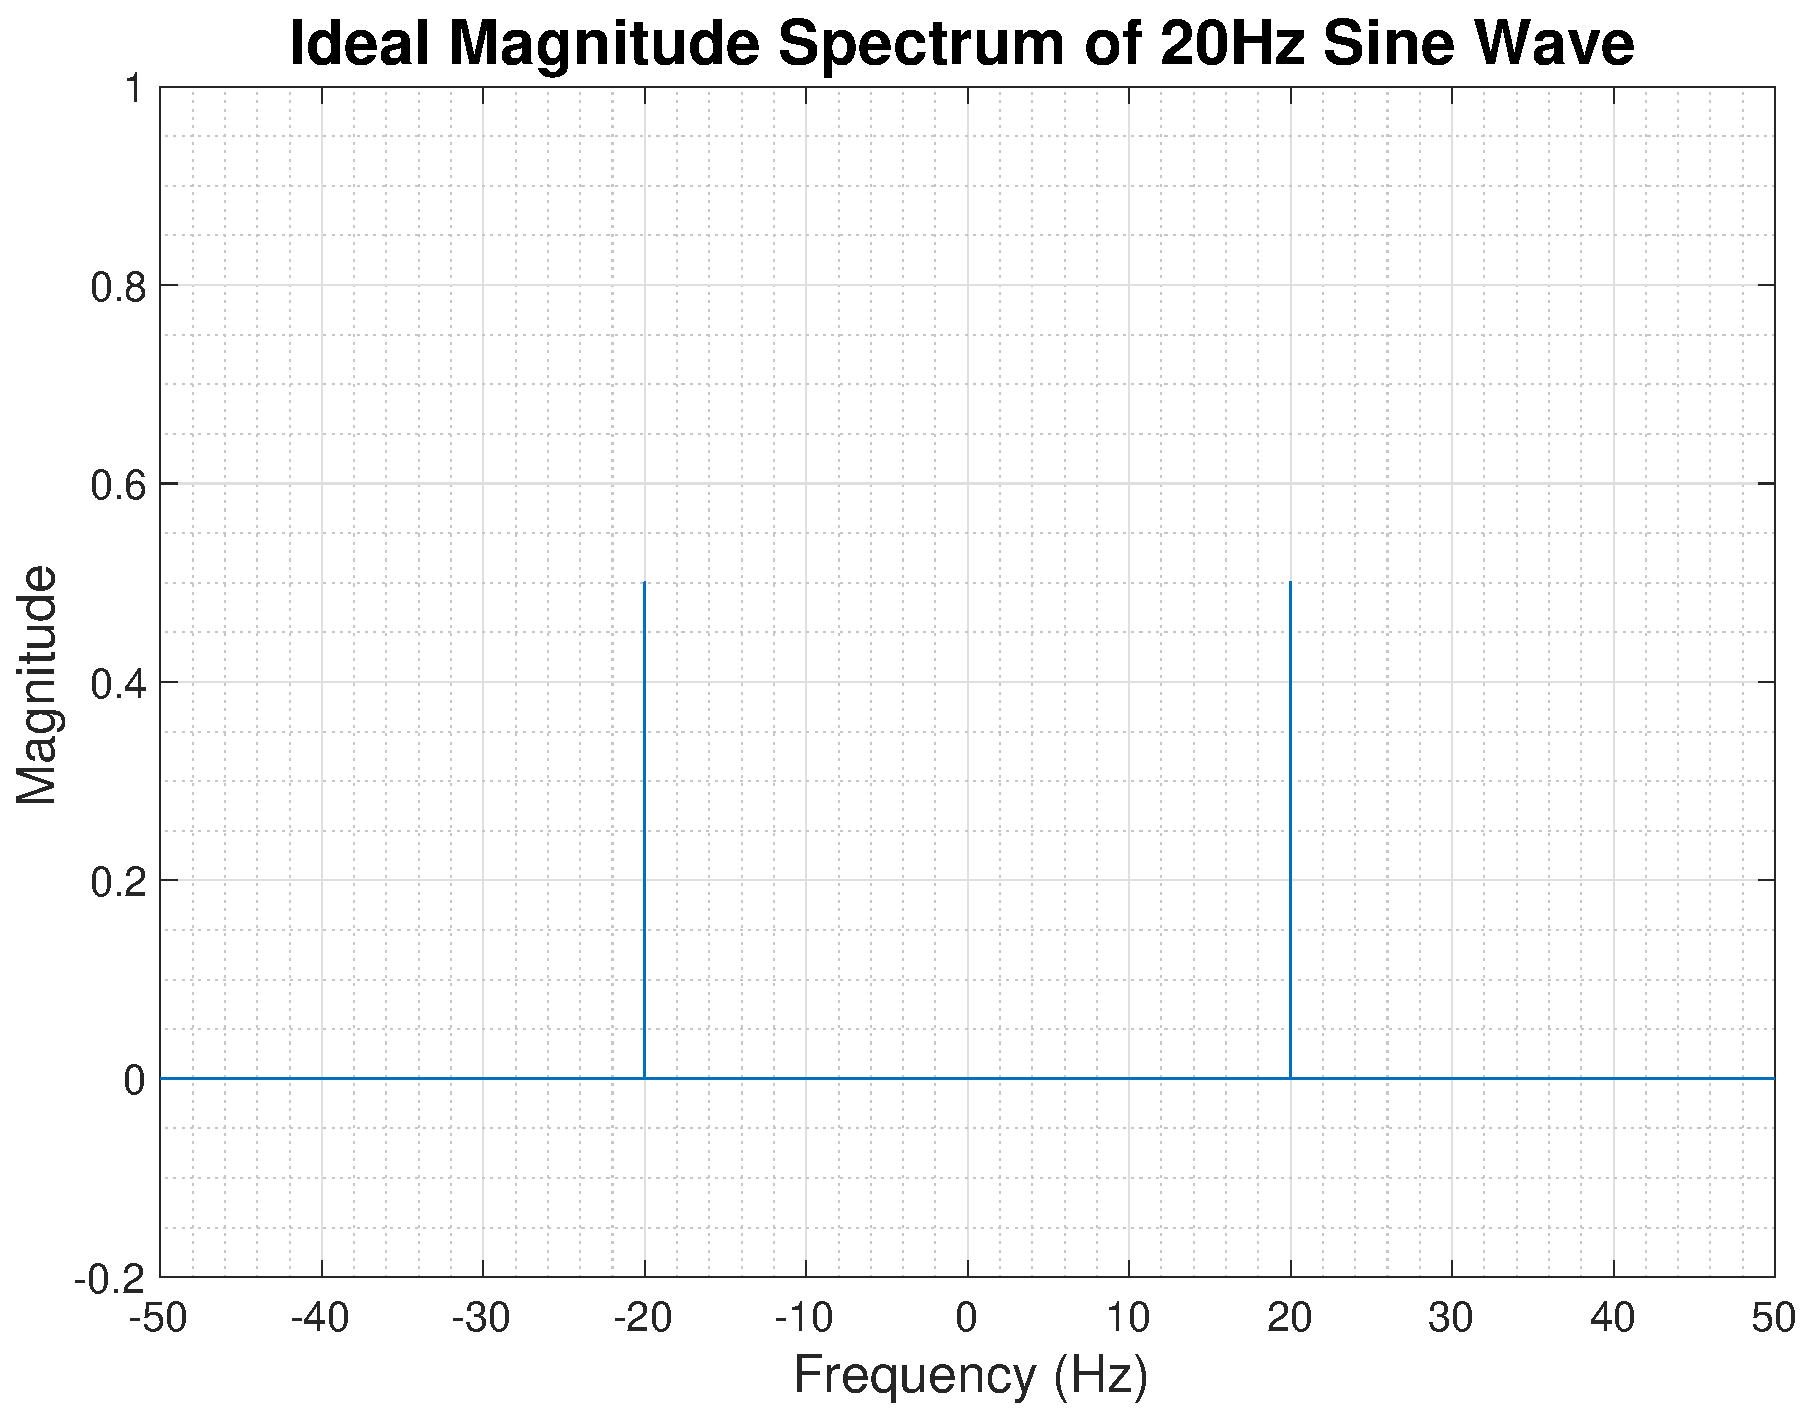
\includegraphics[width=0.49\textwidth]{part1/ideal_magnitude_spectrum_20hz_sine_wave}
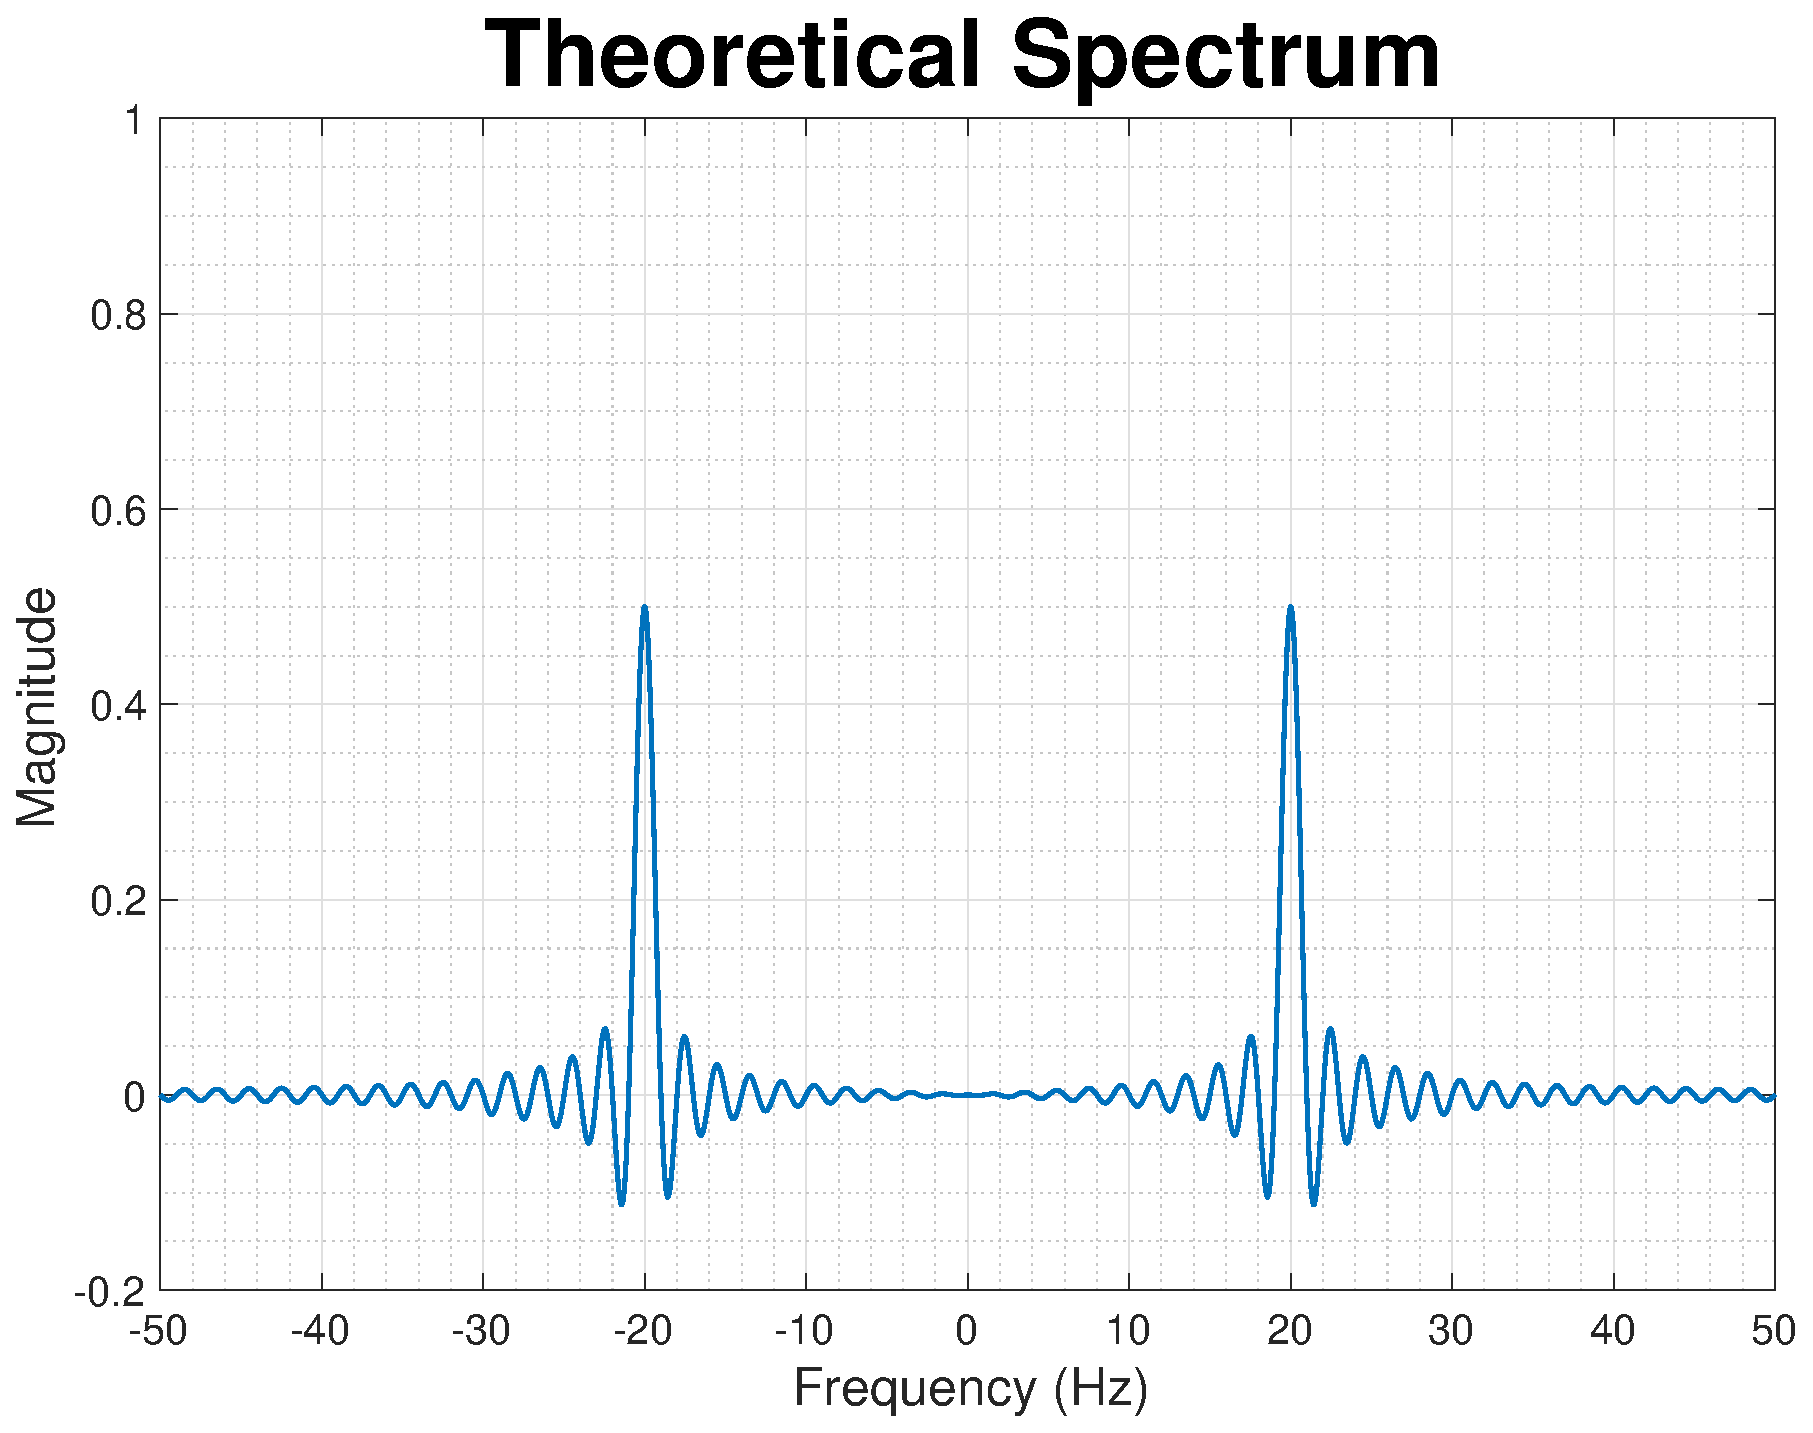
\includegraphics[width=0.49\textwidth]{part1/theoretical_magnitude_spectrum_windowed_20hz_sine_wave}
\label{fig:ideal_and_theoretical_spectra_f_20}
\caption{Ideal magnitude spectrum and Theoretical Continuous DTFT of 20 Hz sine wave}
\end{figure}

\noindent{}b. At first sight, it looks like the DFT spectrum on the left in Figure \ref{fig:dft_spectra_f_20} is exactly the same as ideal spectrum of a 20 Hz sine wave. However, we know that this cannot be the case. The ideal spectrum is derived from a continuous infinite duration sine wave whereas the spectra presented below are both derived from finite duration discrete-time sine waves. In fact, both the spectra below are sampled versions of the theoretical continuous frequency DTFT (magnitude) spectrum shown in Figure \ref{fig:ideal_and_theoretical_spectra_f_20}. The resemble described above comes from the fact that sampling is done in such a way so as to correspond to the x-intercepts exactly. The rectangular window used to limit is signal is 0.1 s long and thus the sinc function will have intercepts at $f=1/0.1=10 Hz$. 100 samples are evenly divided across an axis that is 1000 Hz long and thus, each sample is separated by 10 Hz and exactly corresponds to frequencies for which the sinc function is 0, expect at frequencies -20 Hz and 20 Hz. The side lobes that come about due to the rectangular window become evident when more points from the continuous DTFT spectrum are sampled.

\begin{figure}[H]
\centering{}
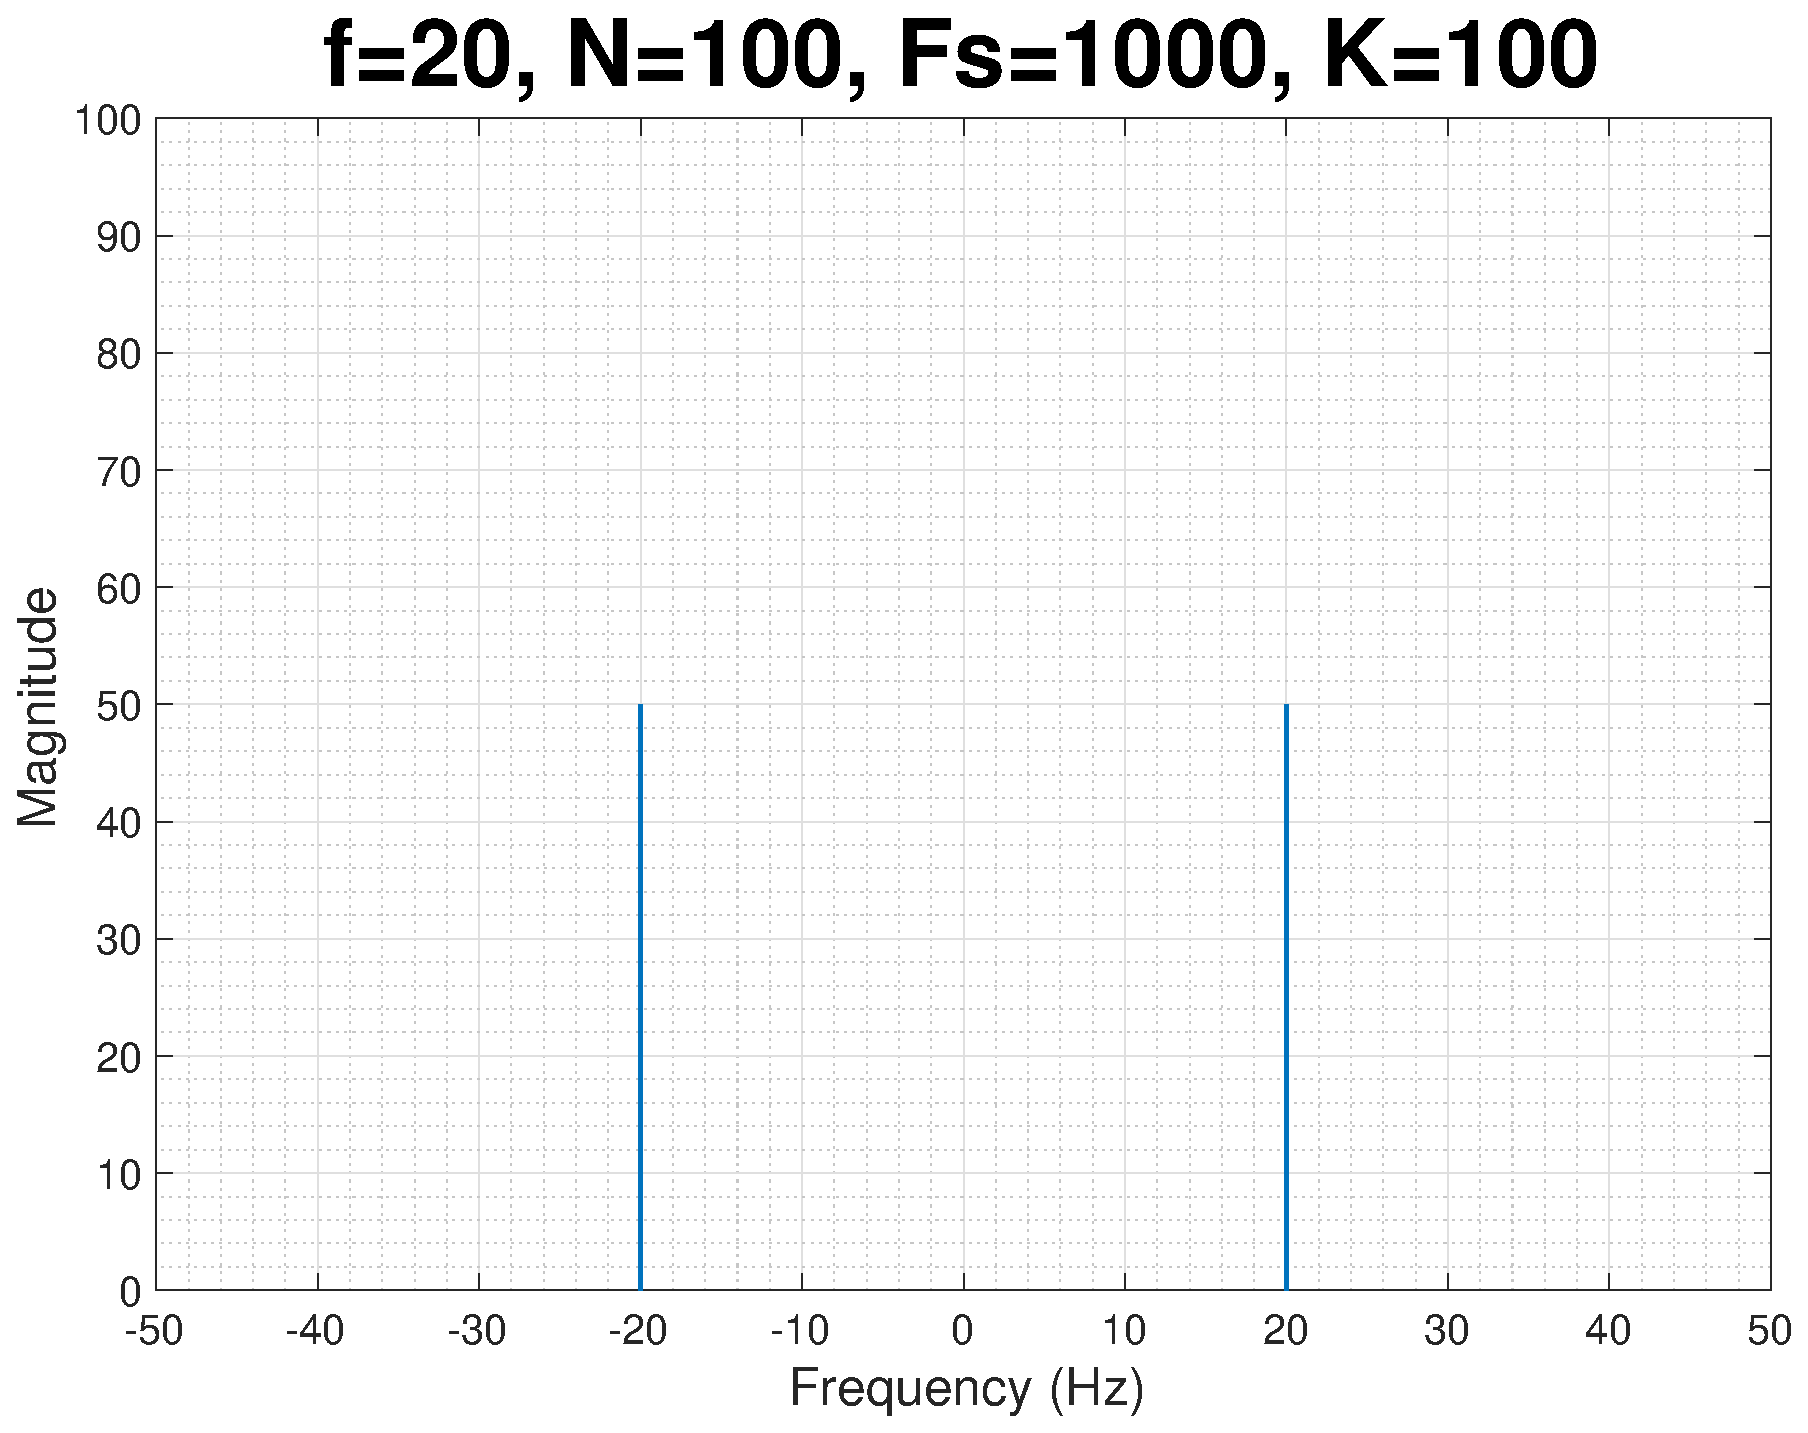
\includegraphics[width=0.49\textwidth]{part1/dft_spectra_f_20_n_100_Fs_1000_k_100}
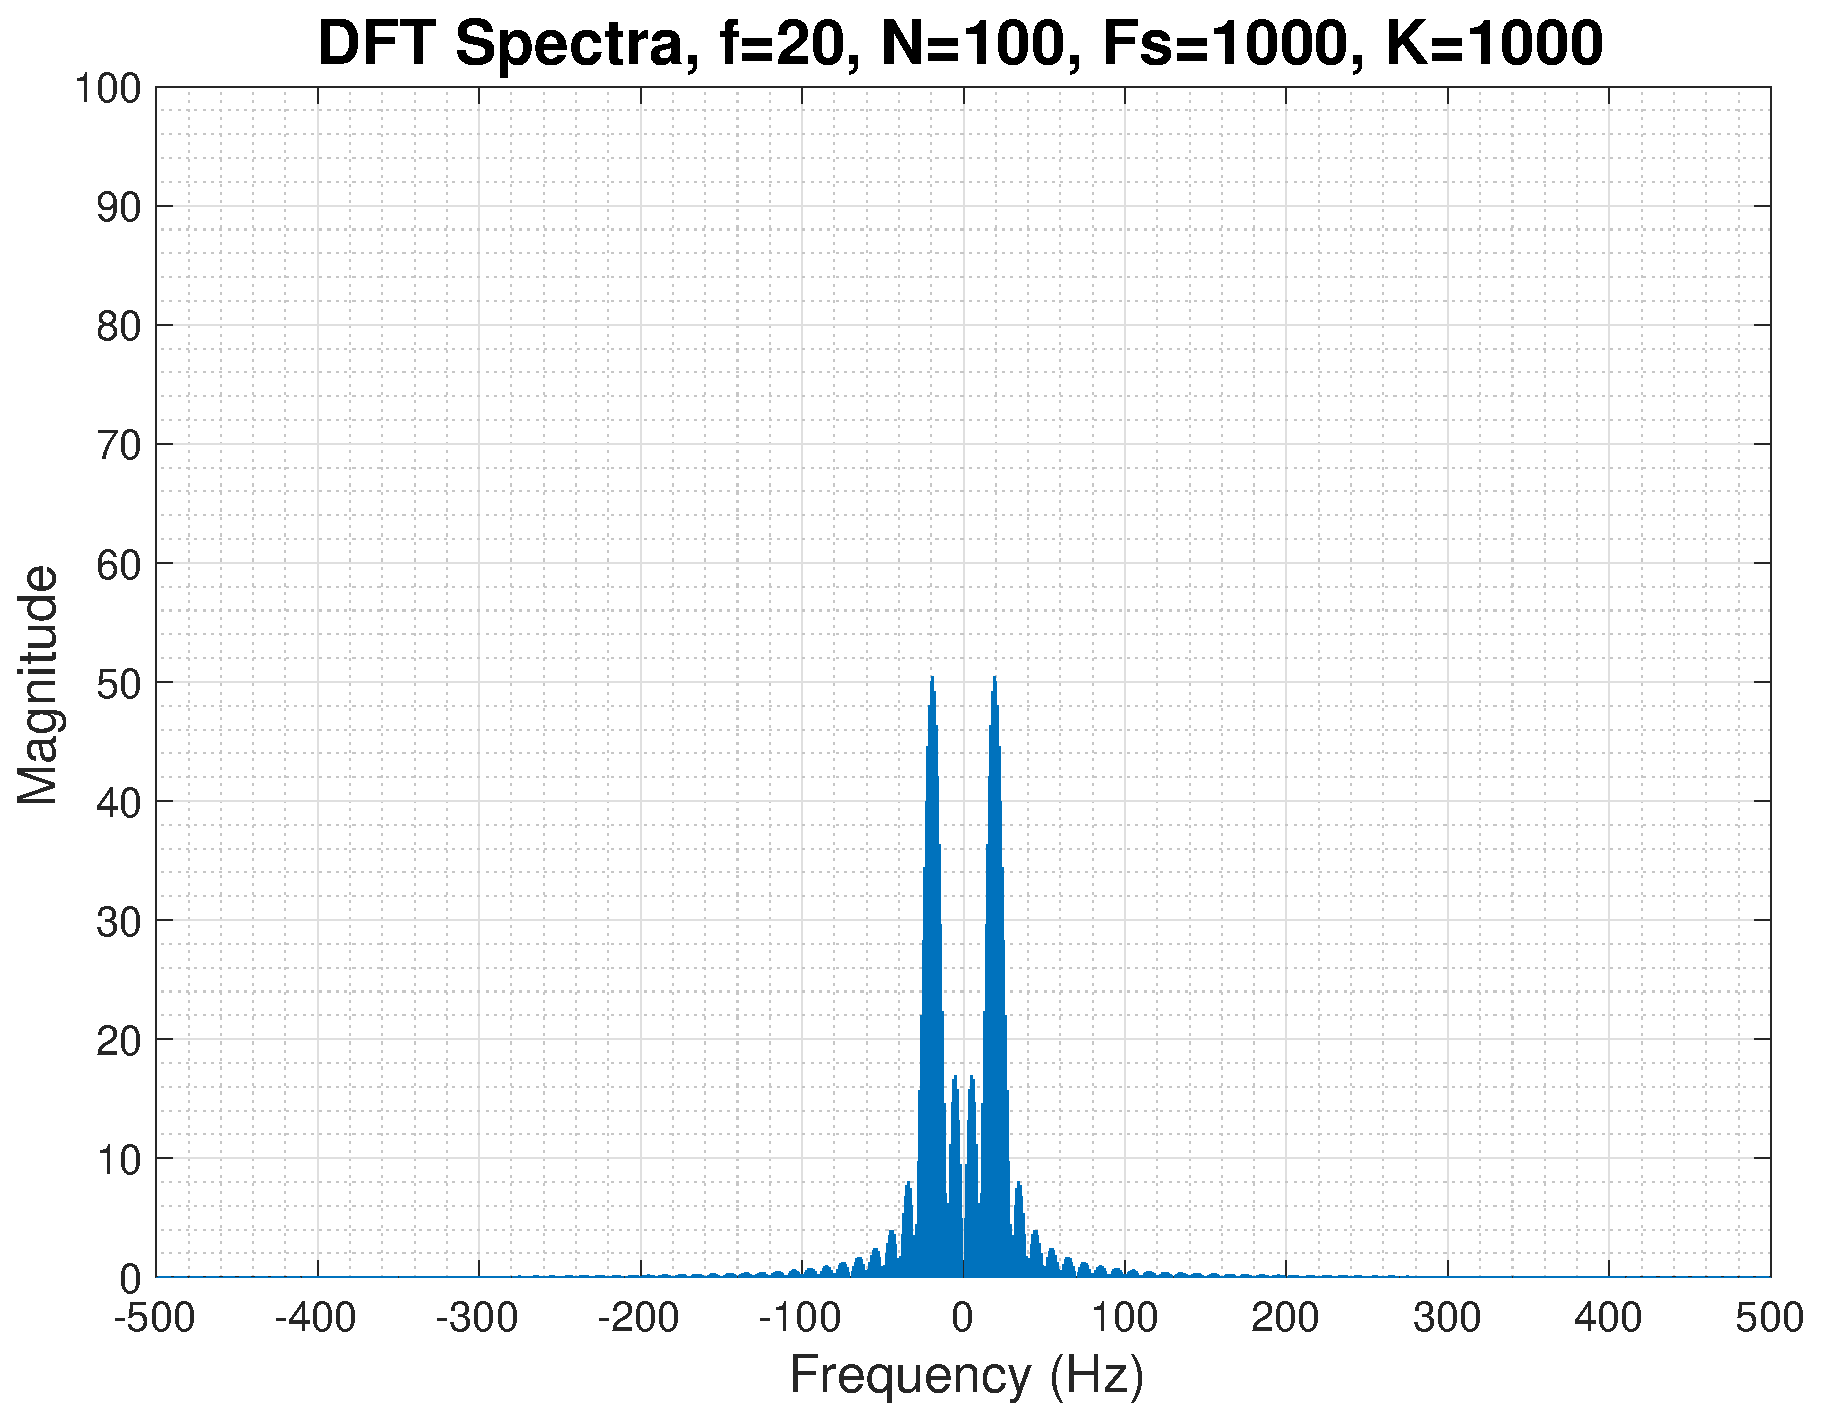
\includegraphics[width=0.49\textwidth]{part1/dft_spectra_f_20_n_100_Fs_1000_k_1000}
\label{fig:dft_spectra_f_20}
\caption{Random Caption}
\end{figure}

\noindent{}c. The graphs below show the K-point DFT (magnitude) spectrum for $K=100$ and $K=2^{16}$; the graph on the right was generated using the \texttt{plot} function rather than the \texttt{stem} function since the theoretical continuous frequency DTFT has been sampled so densely that it is effectively continuous. The graphs below illustrate the effects of sampling the continuous frequency DTFT sparsely; the true peaks are not correctly identified. Increasing the value of K can be used to solve the incoherent sampling problem. This is easily obtained by zero-padding the signal.

\begin{figure}[H]
\centering{}
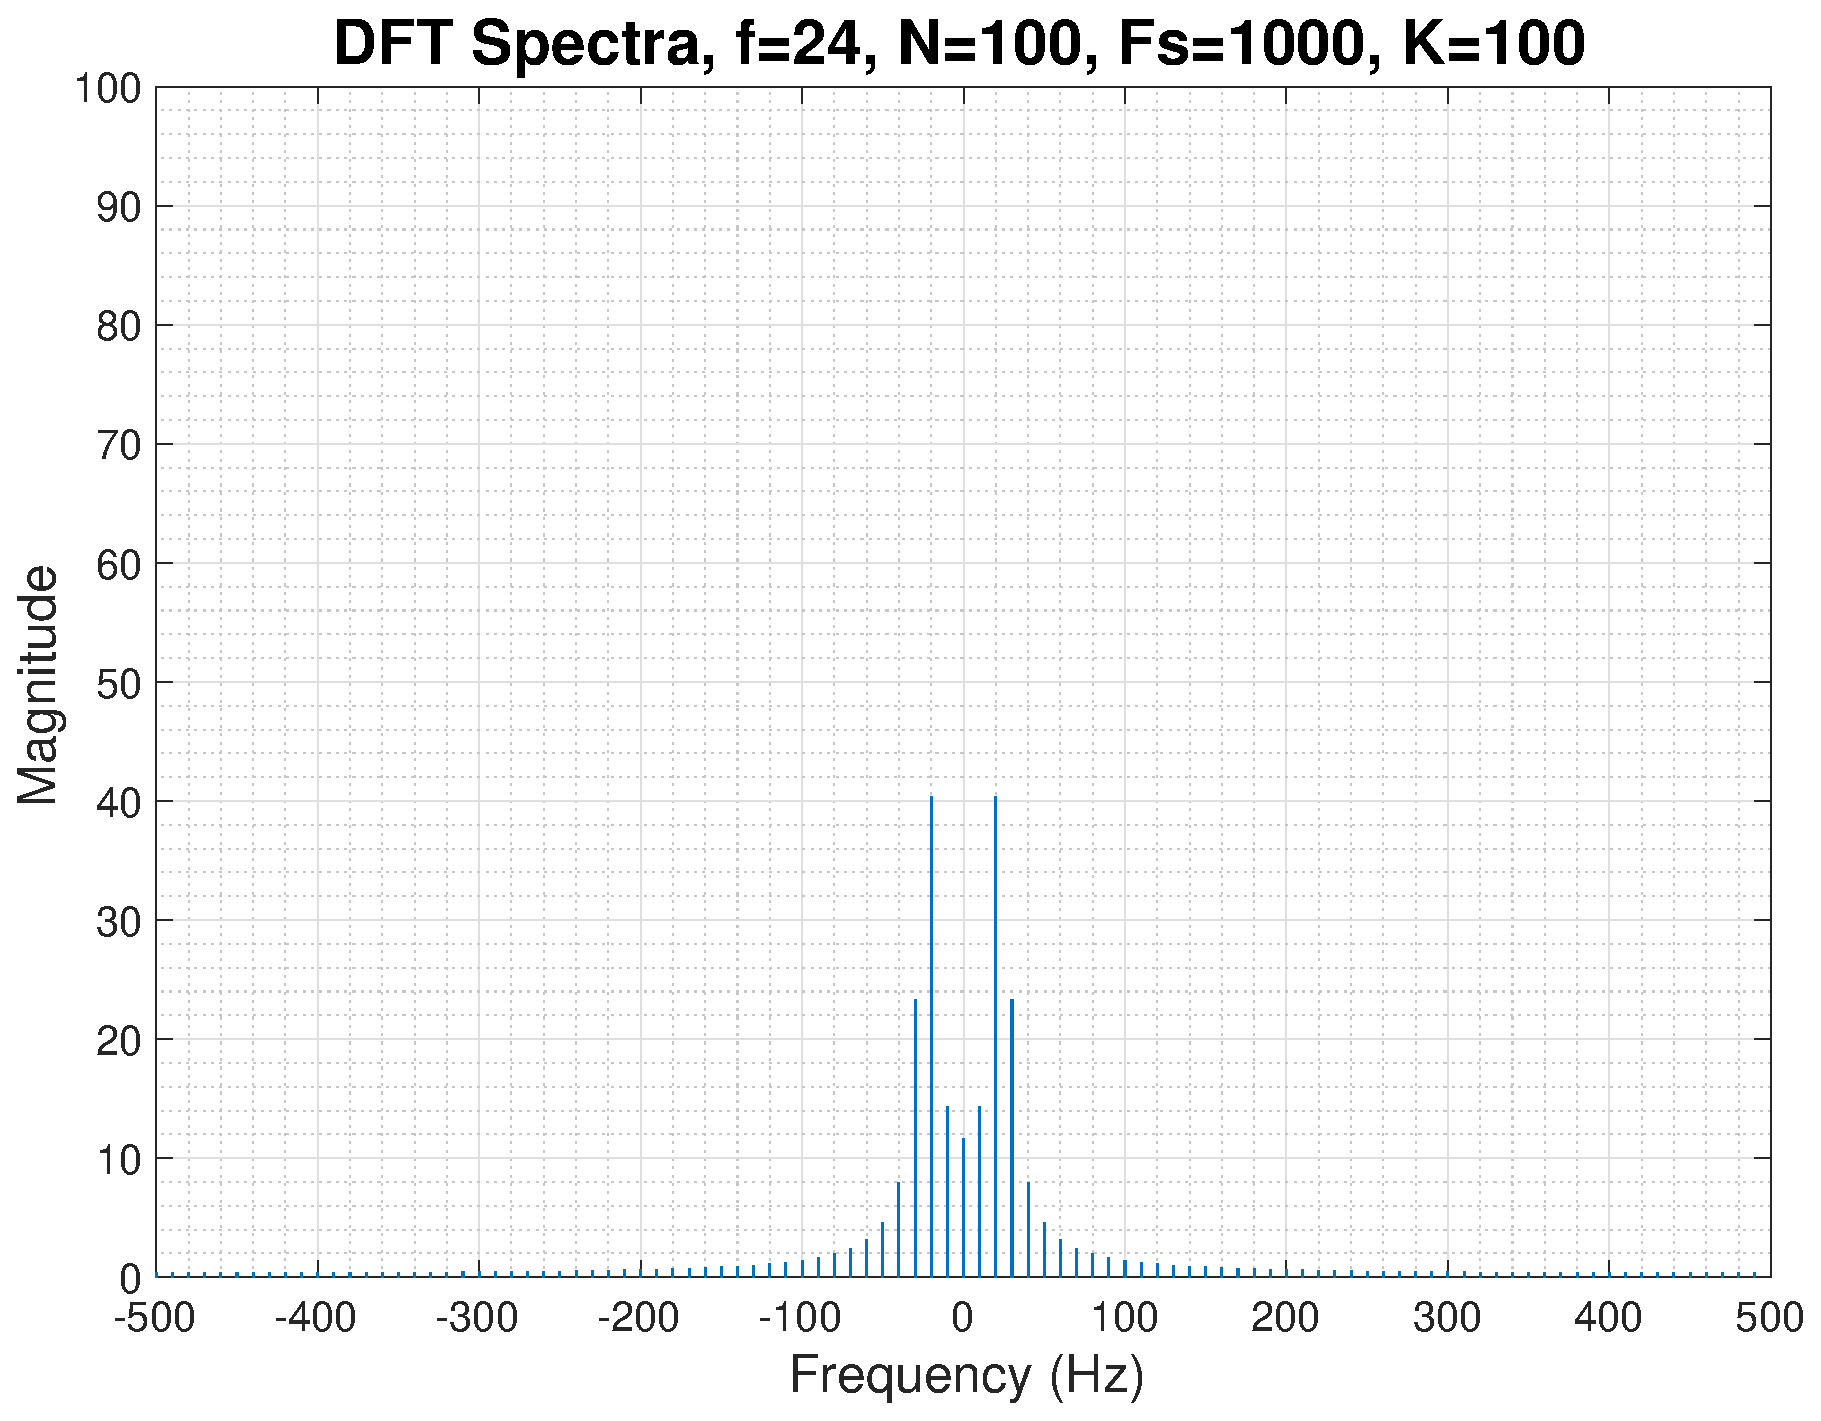
\includegraphics[width=0.49\textwidth]{part1/dft_spectra_f_24_n_100_Fs_1000_k_100}
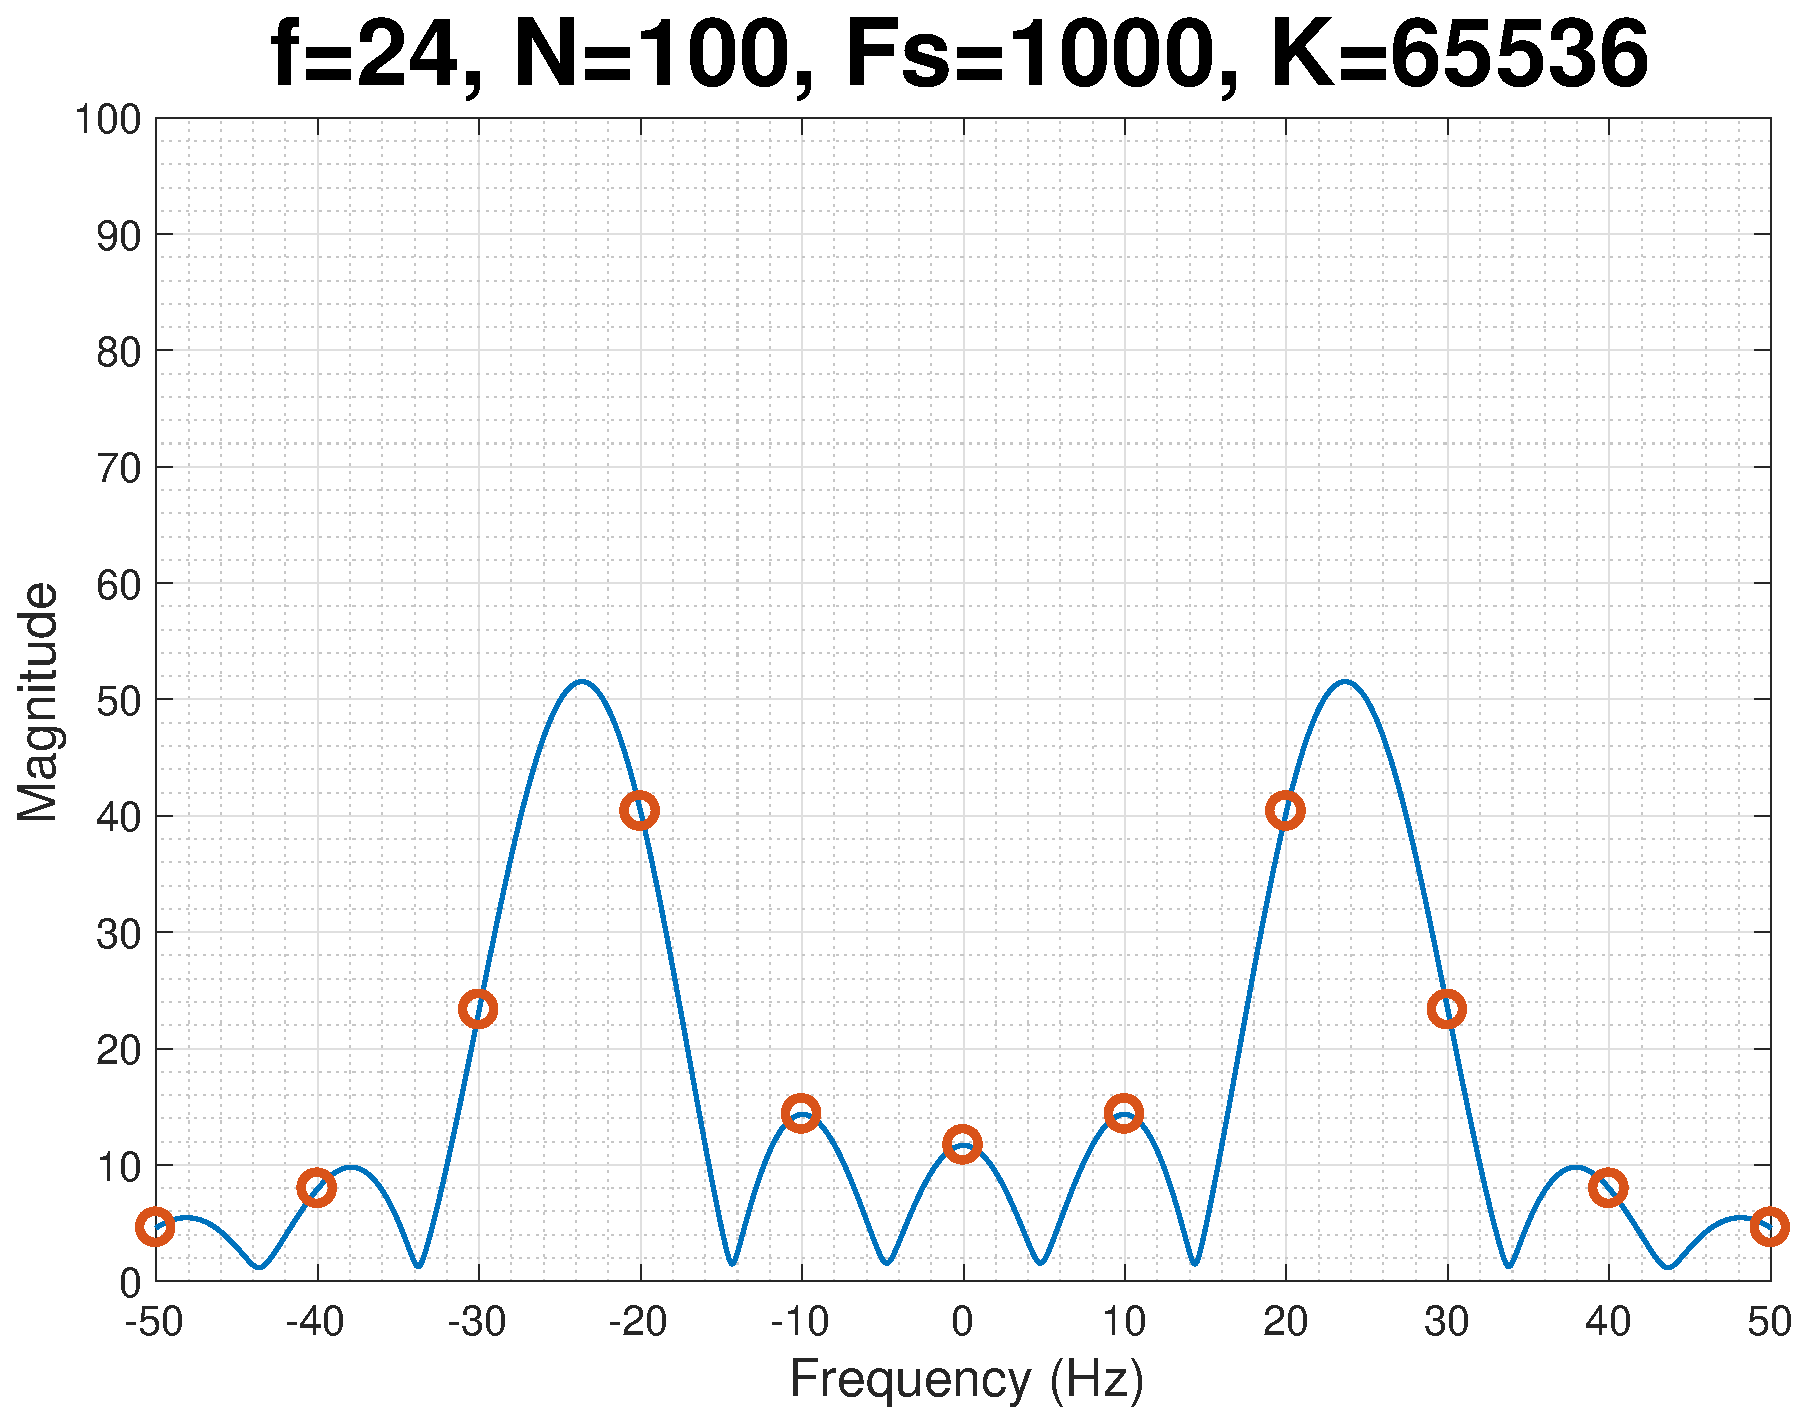
\includegraphics[width=0.49\textwidth]{part1/dft_spectra_f_24_n_100_Fs_1000_k_2_to_16}
\caption{Random Caption}
\end{figure}

\subsection{Properties of Power Spectral Density (PSD)}

\begin{figure}[H]
\centering{}
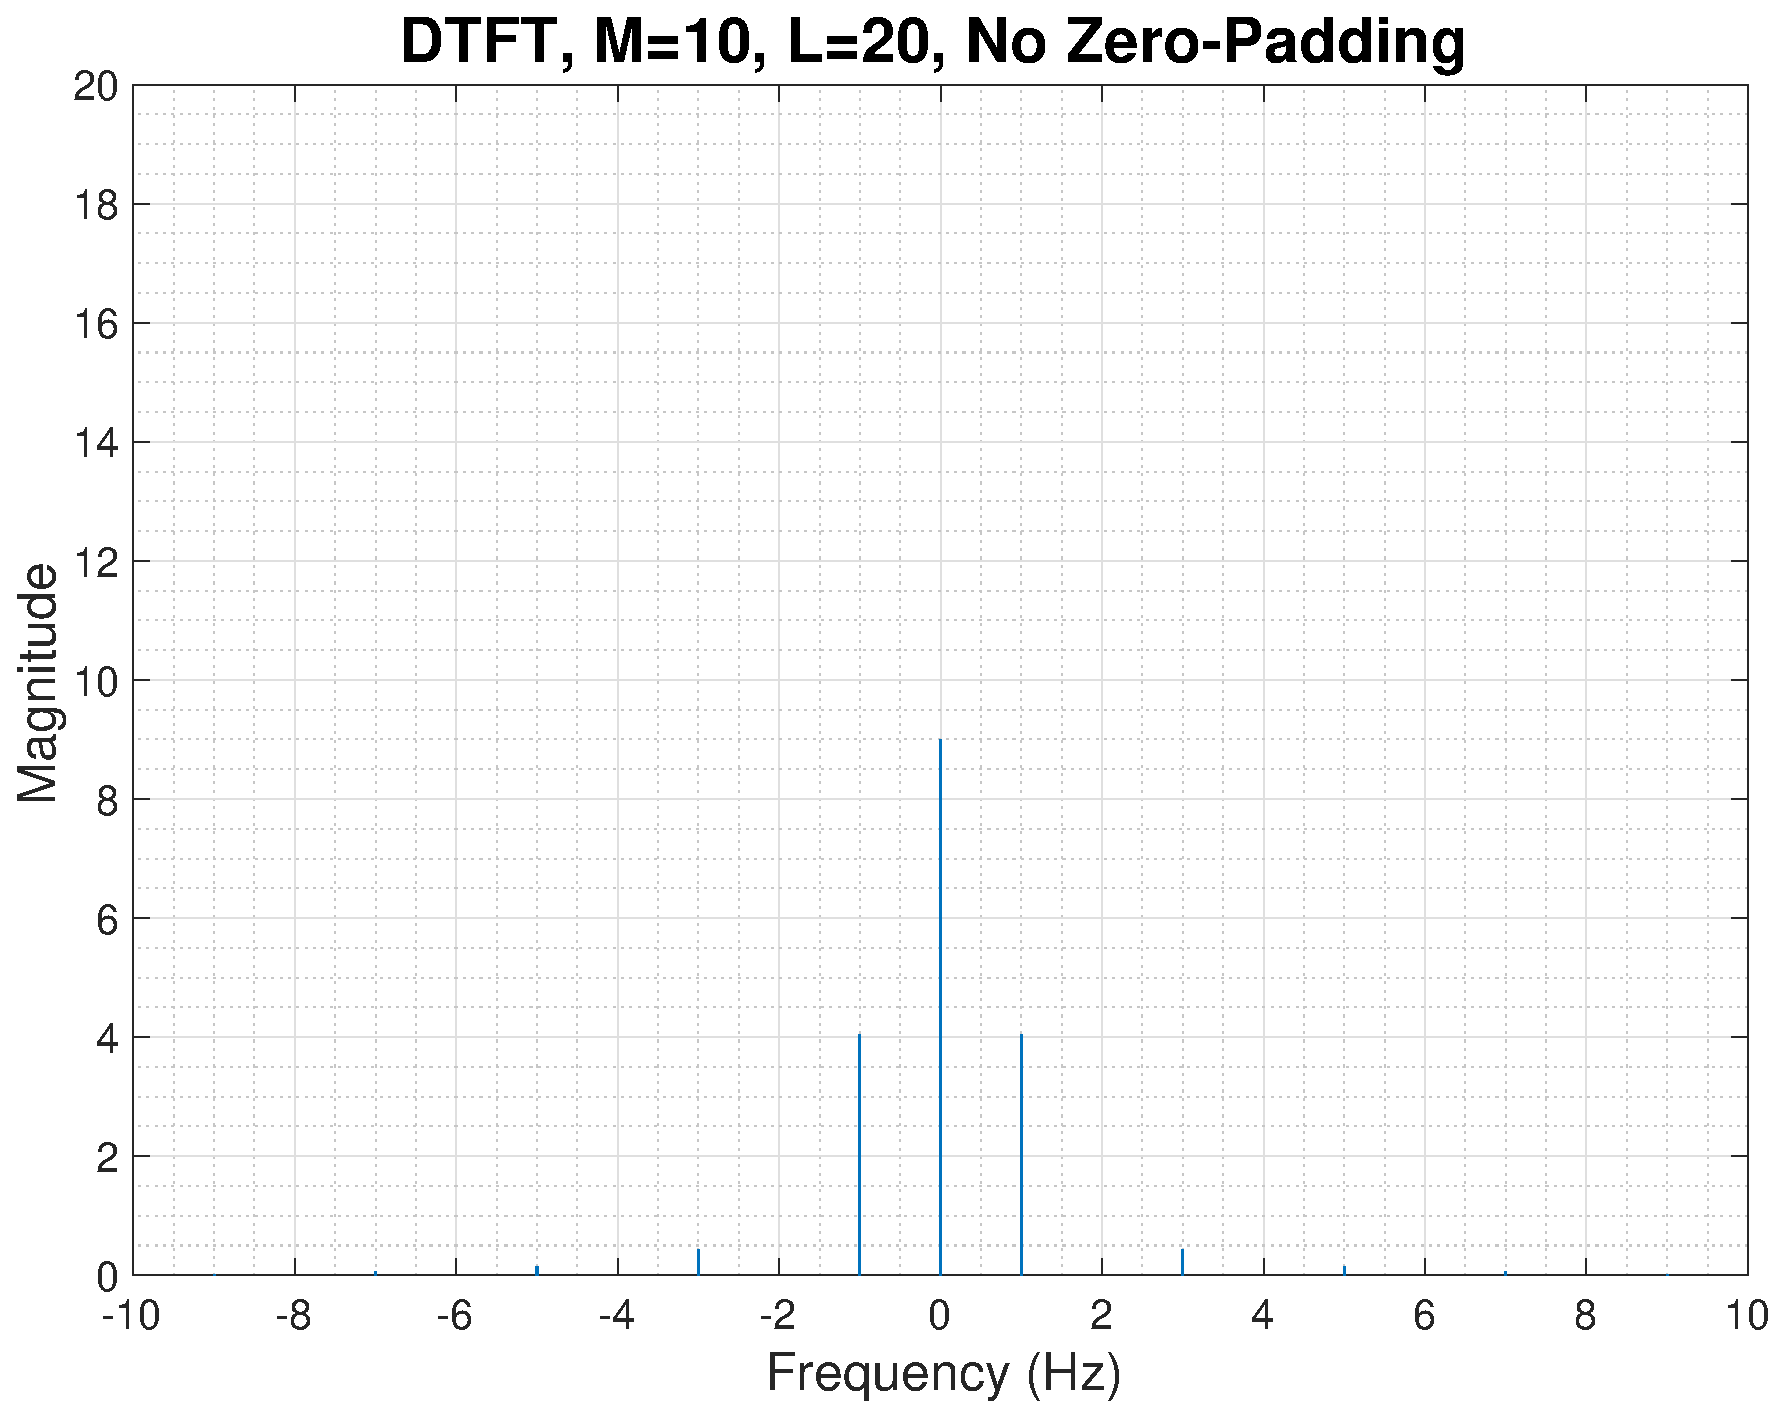
\includegraphics[width=0.49\textwidth]{part1/dft_spectra_acf_m_10_l_20}
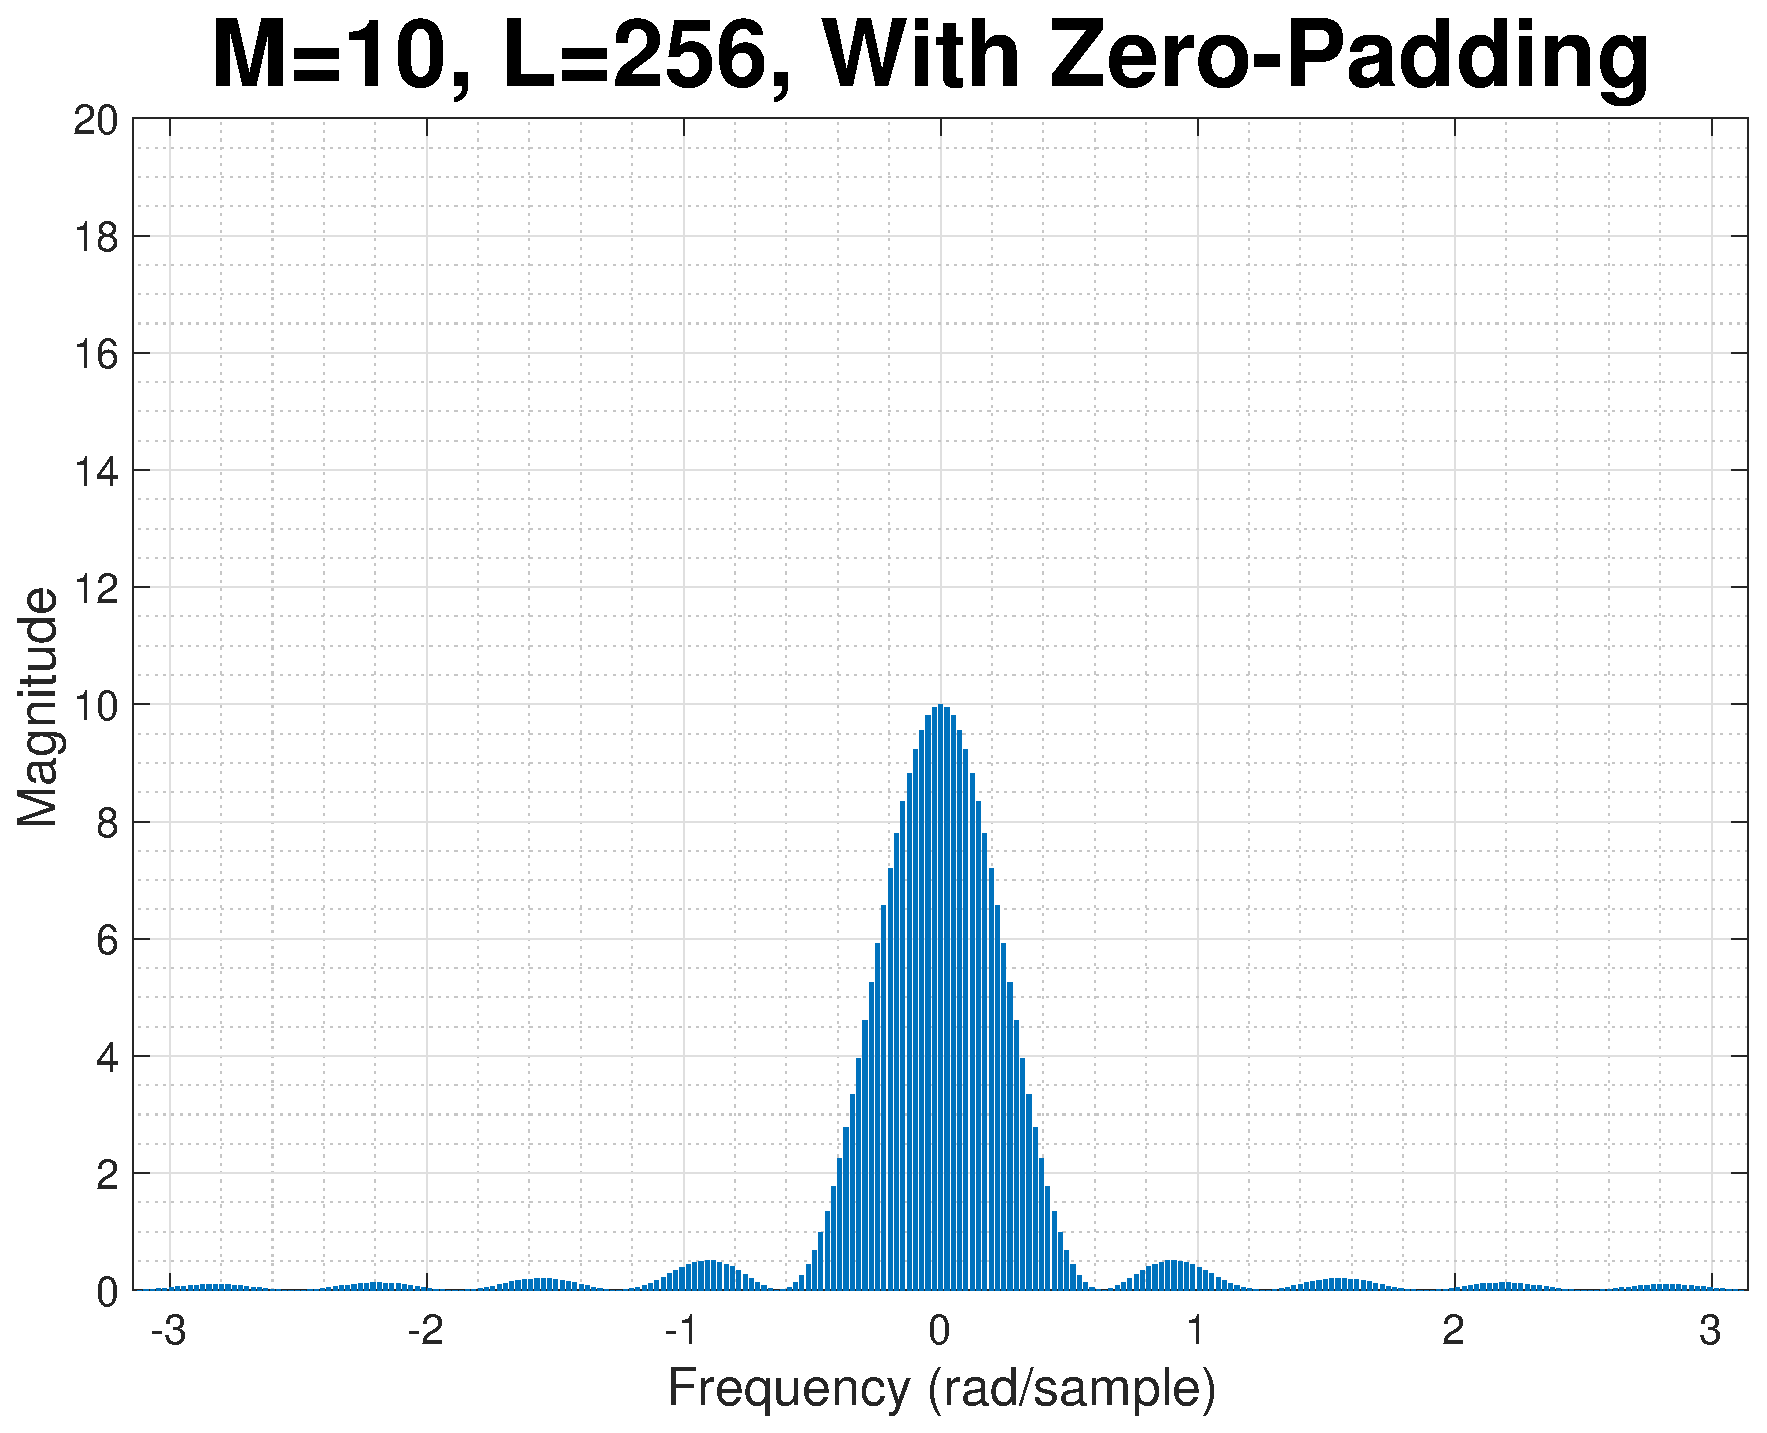
\includegraphics[width=0.49\textwidth]{part1/dft_spectra_acf_m_10_l_256}
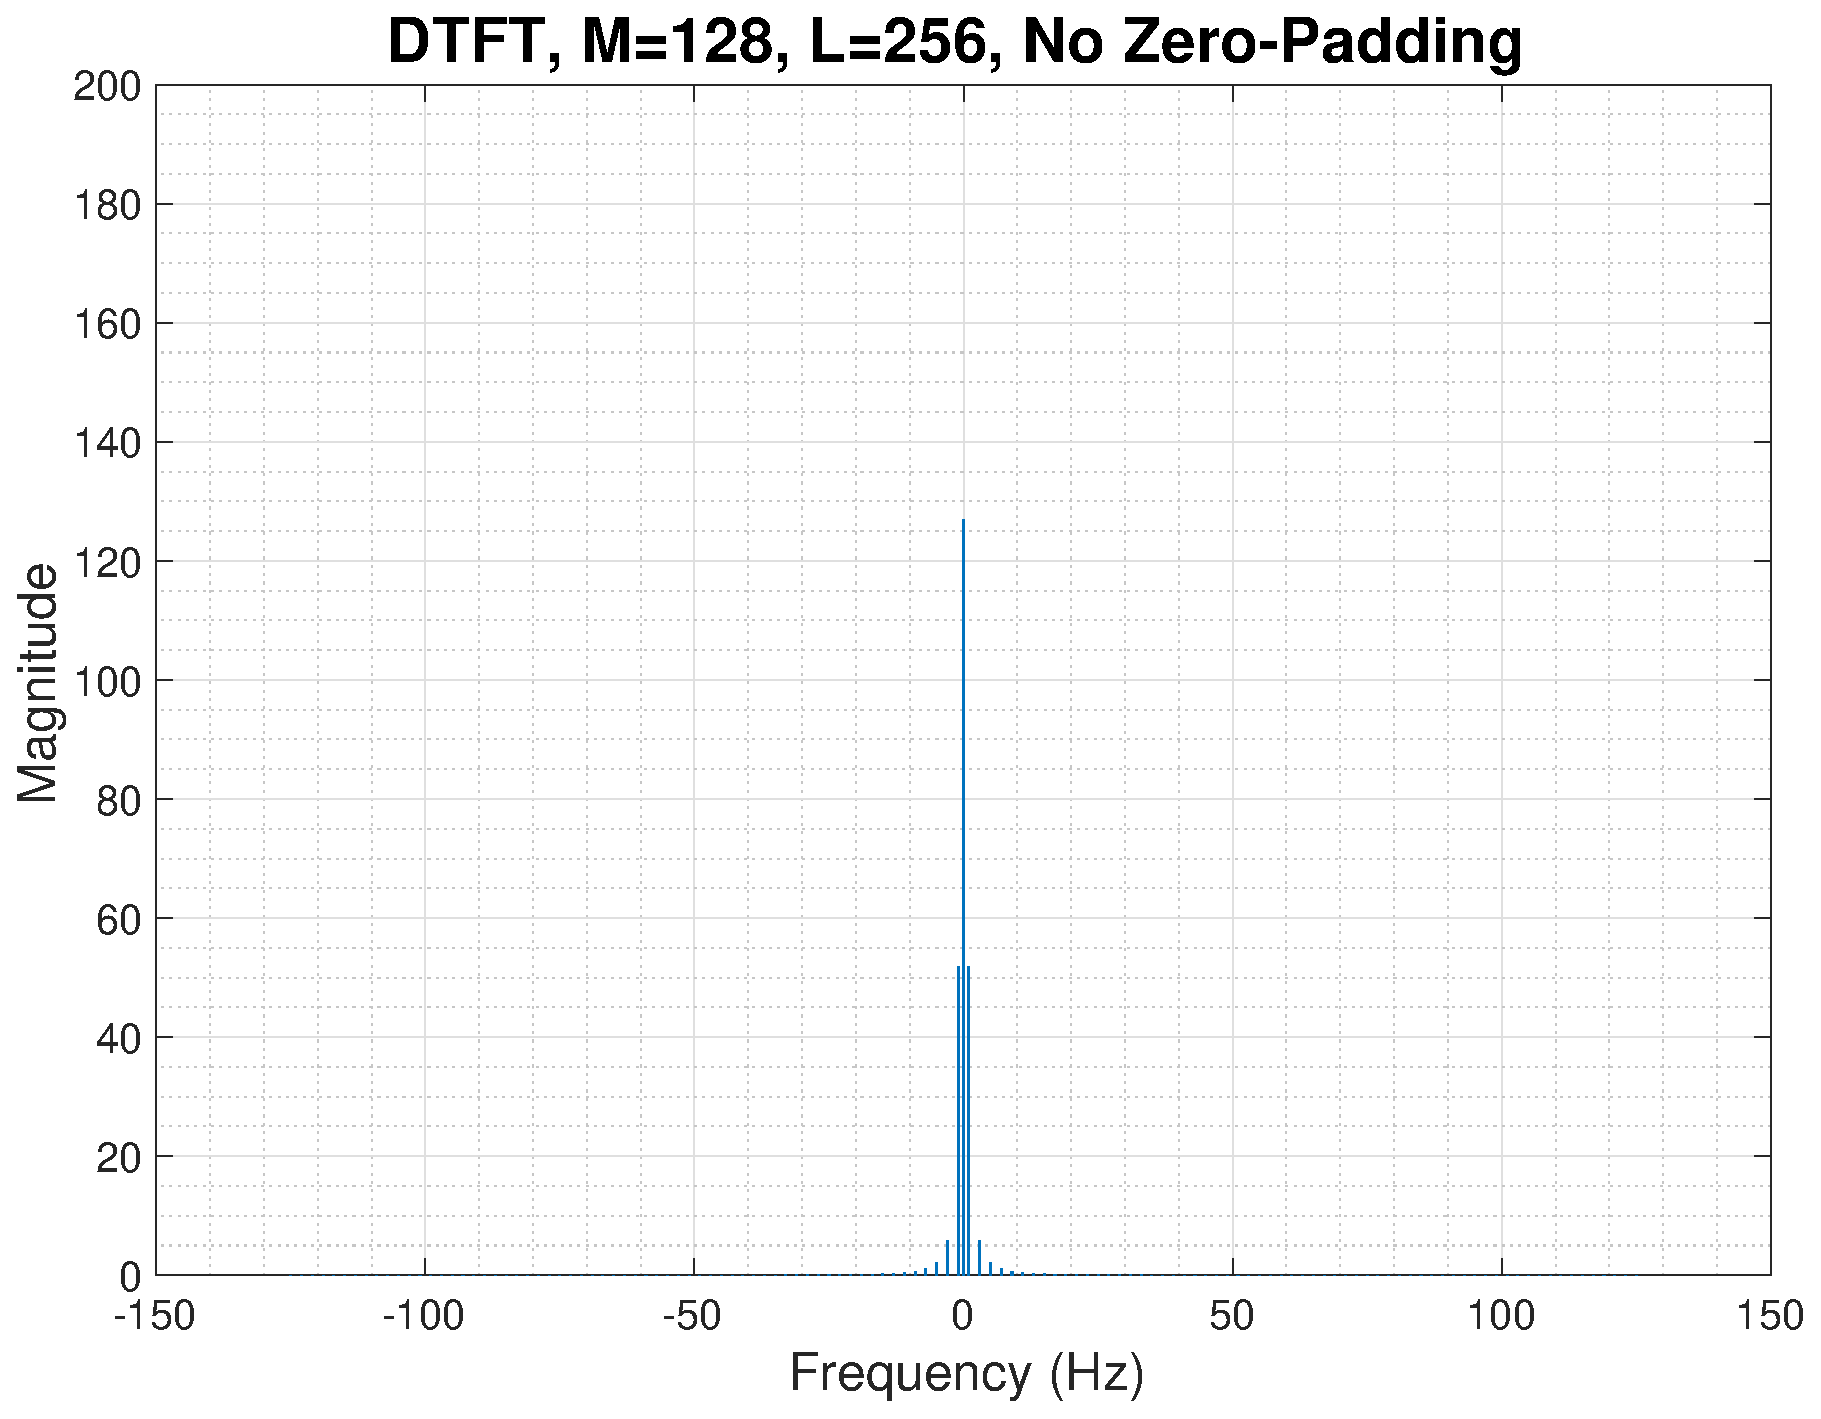
\includegraphics[width=0.49\textwidth]{part1/dft_spectra_acf_m_128_l_256}
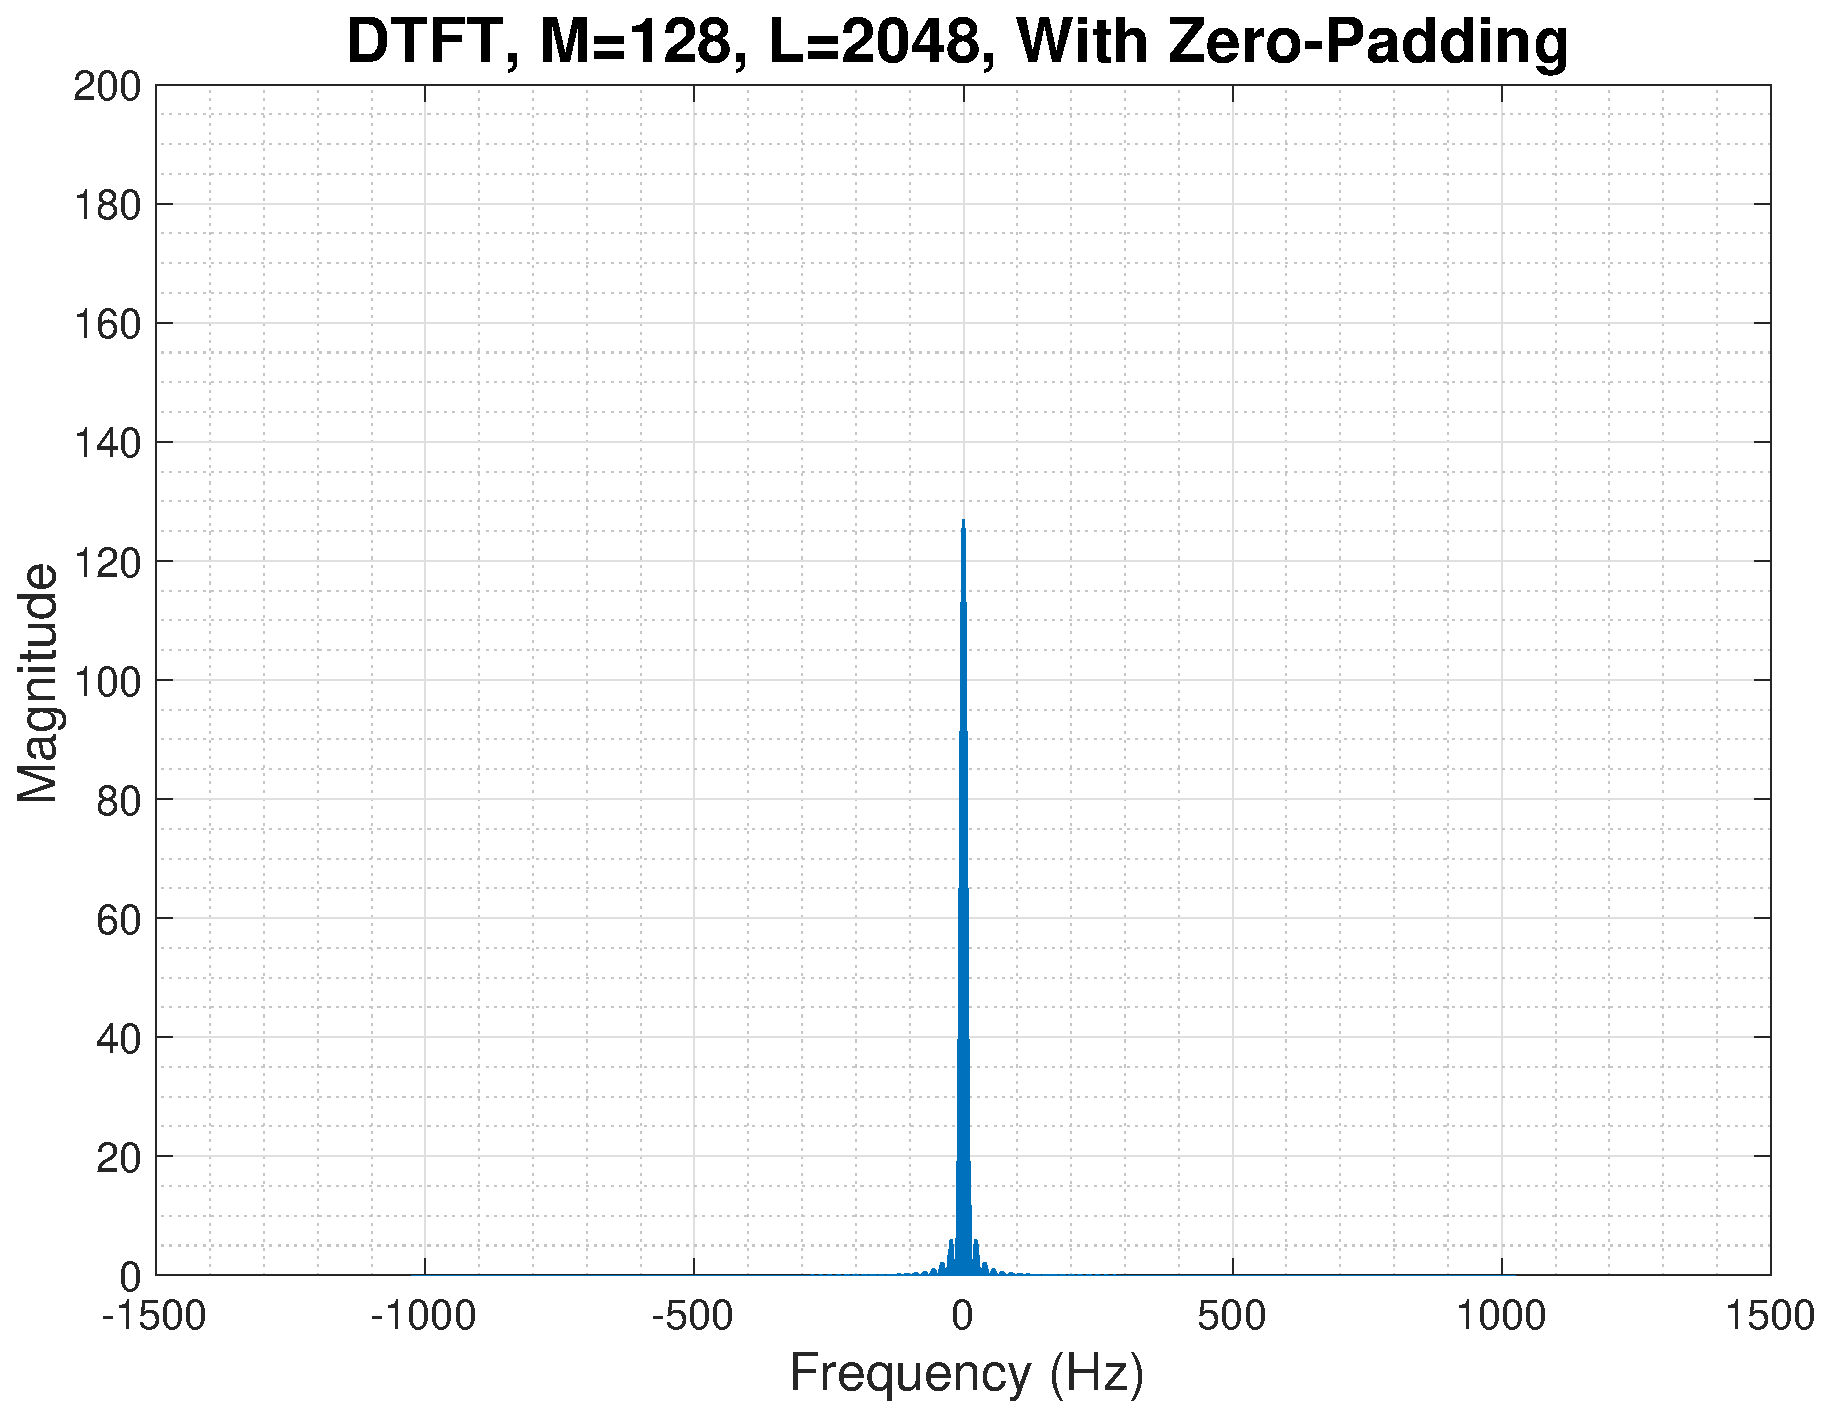
\includegraphics[width=0.49\textwidth]{part1/dft_spectra_acf_m_128_l_2048}
\caption{Random Caption}
\end{figure}


\begin{figure}[H]
\centering{}
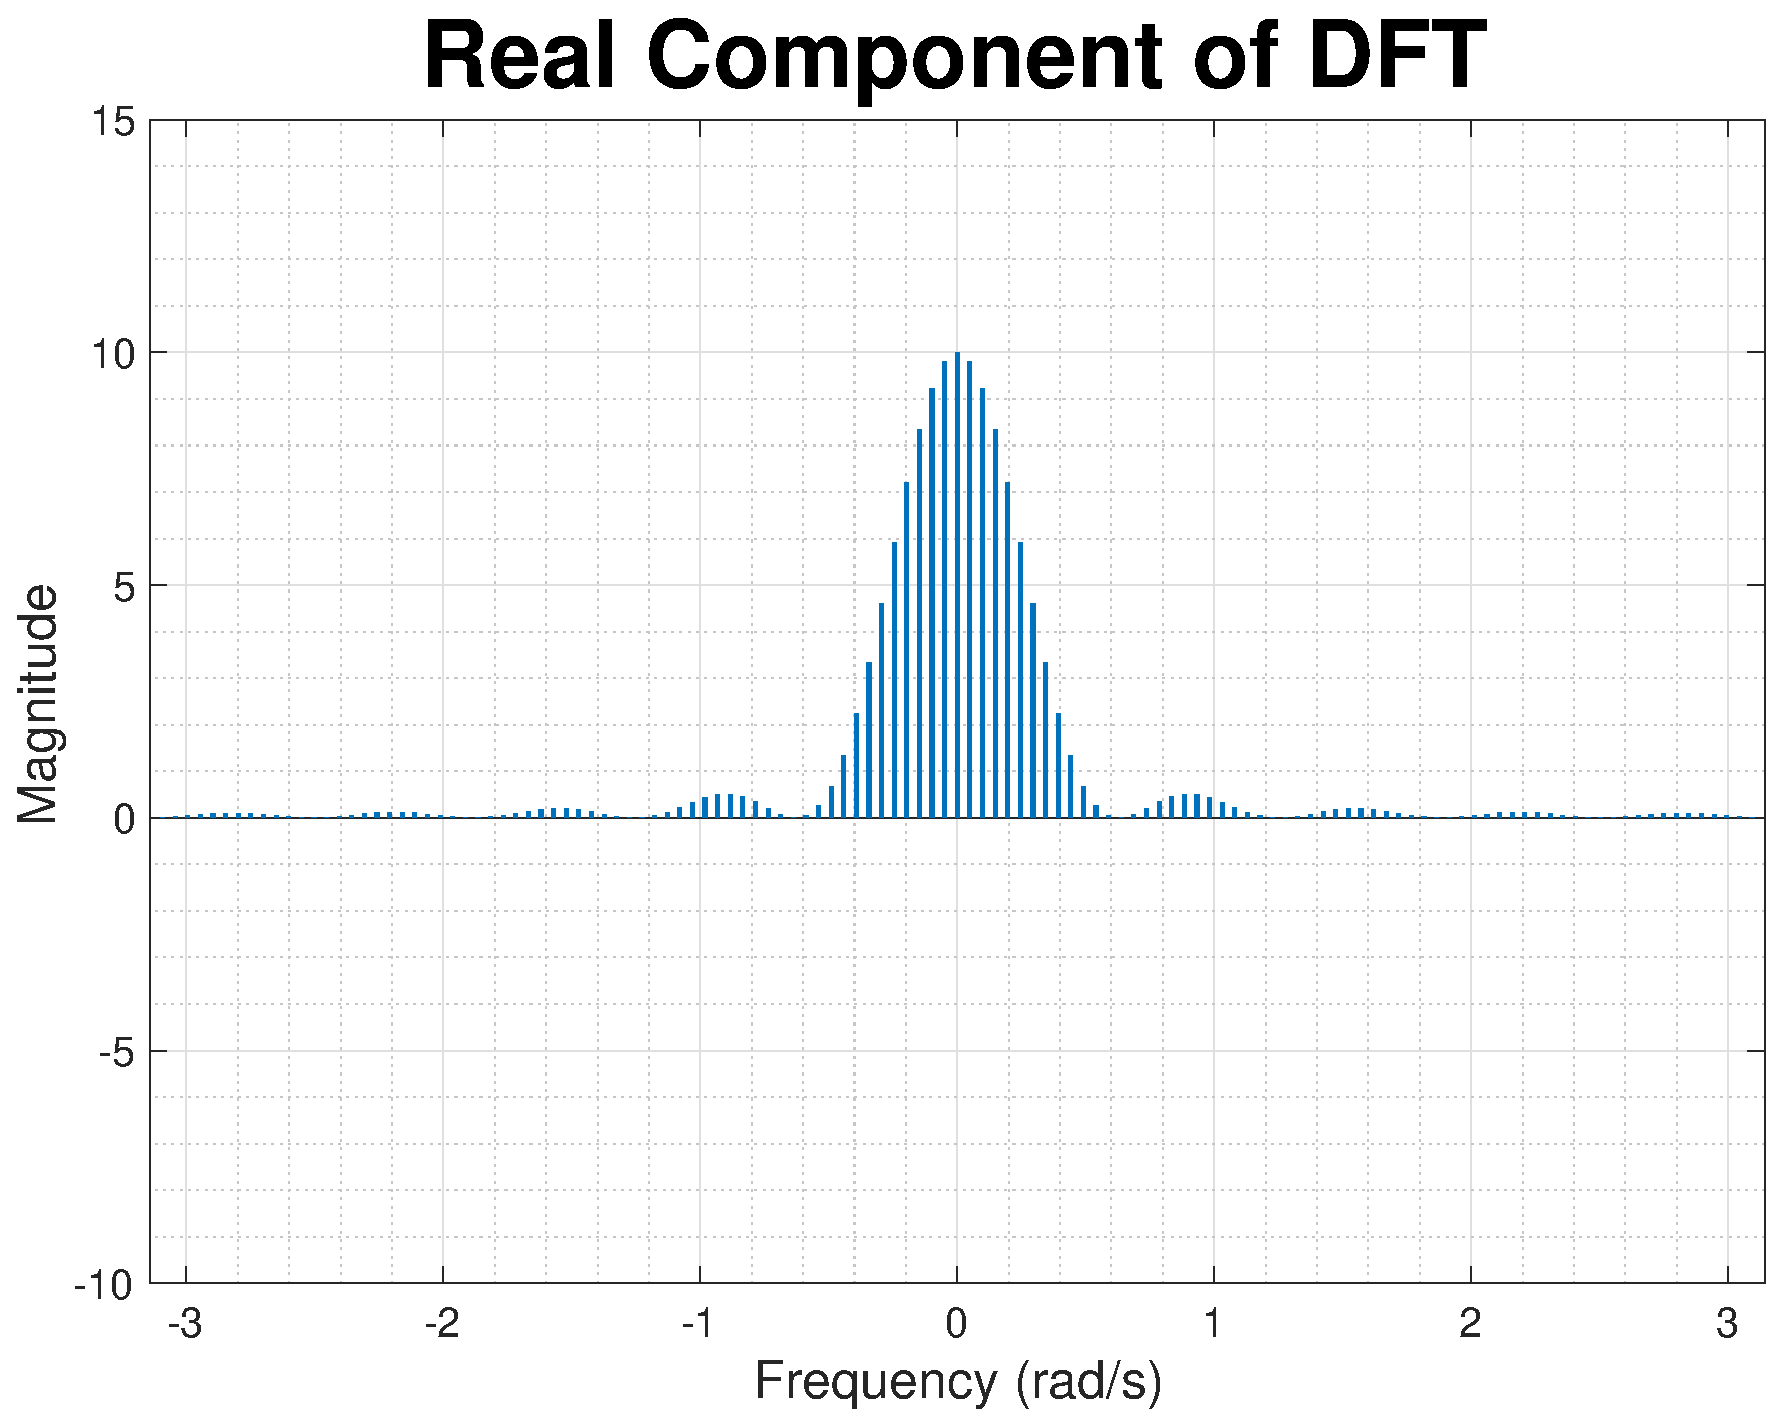
\includegraphics[width=0.49\textwidth]{part1/dft_spectra_acf_x_real}
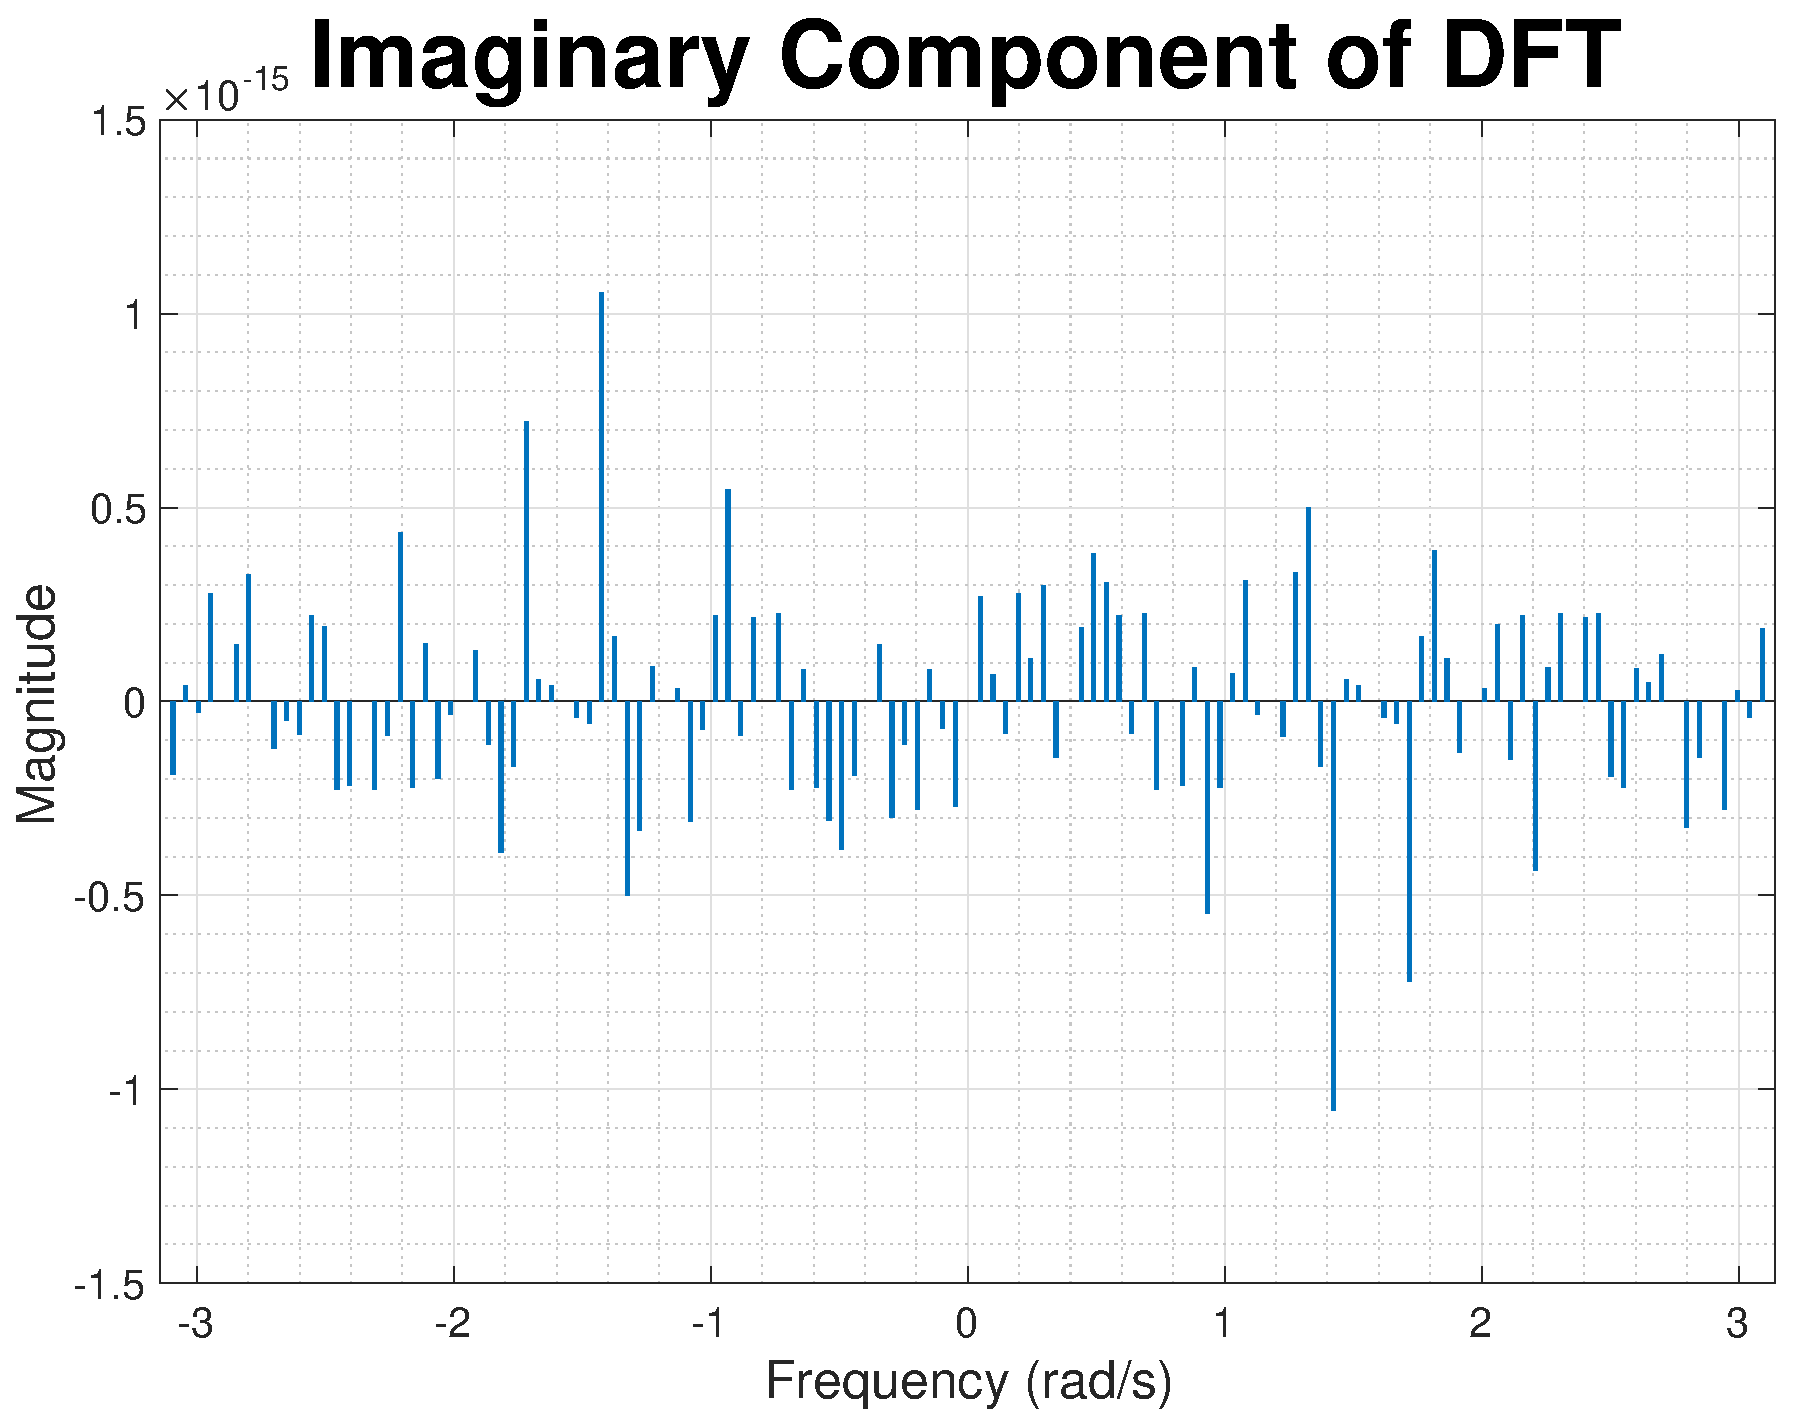
\includegraphics[width=0.49\textwidth]{part1/dft_spectra_acf_x_imag}
\caption{Random Caption}
\end{figure}


\begin{figure}[H]
\centering{}
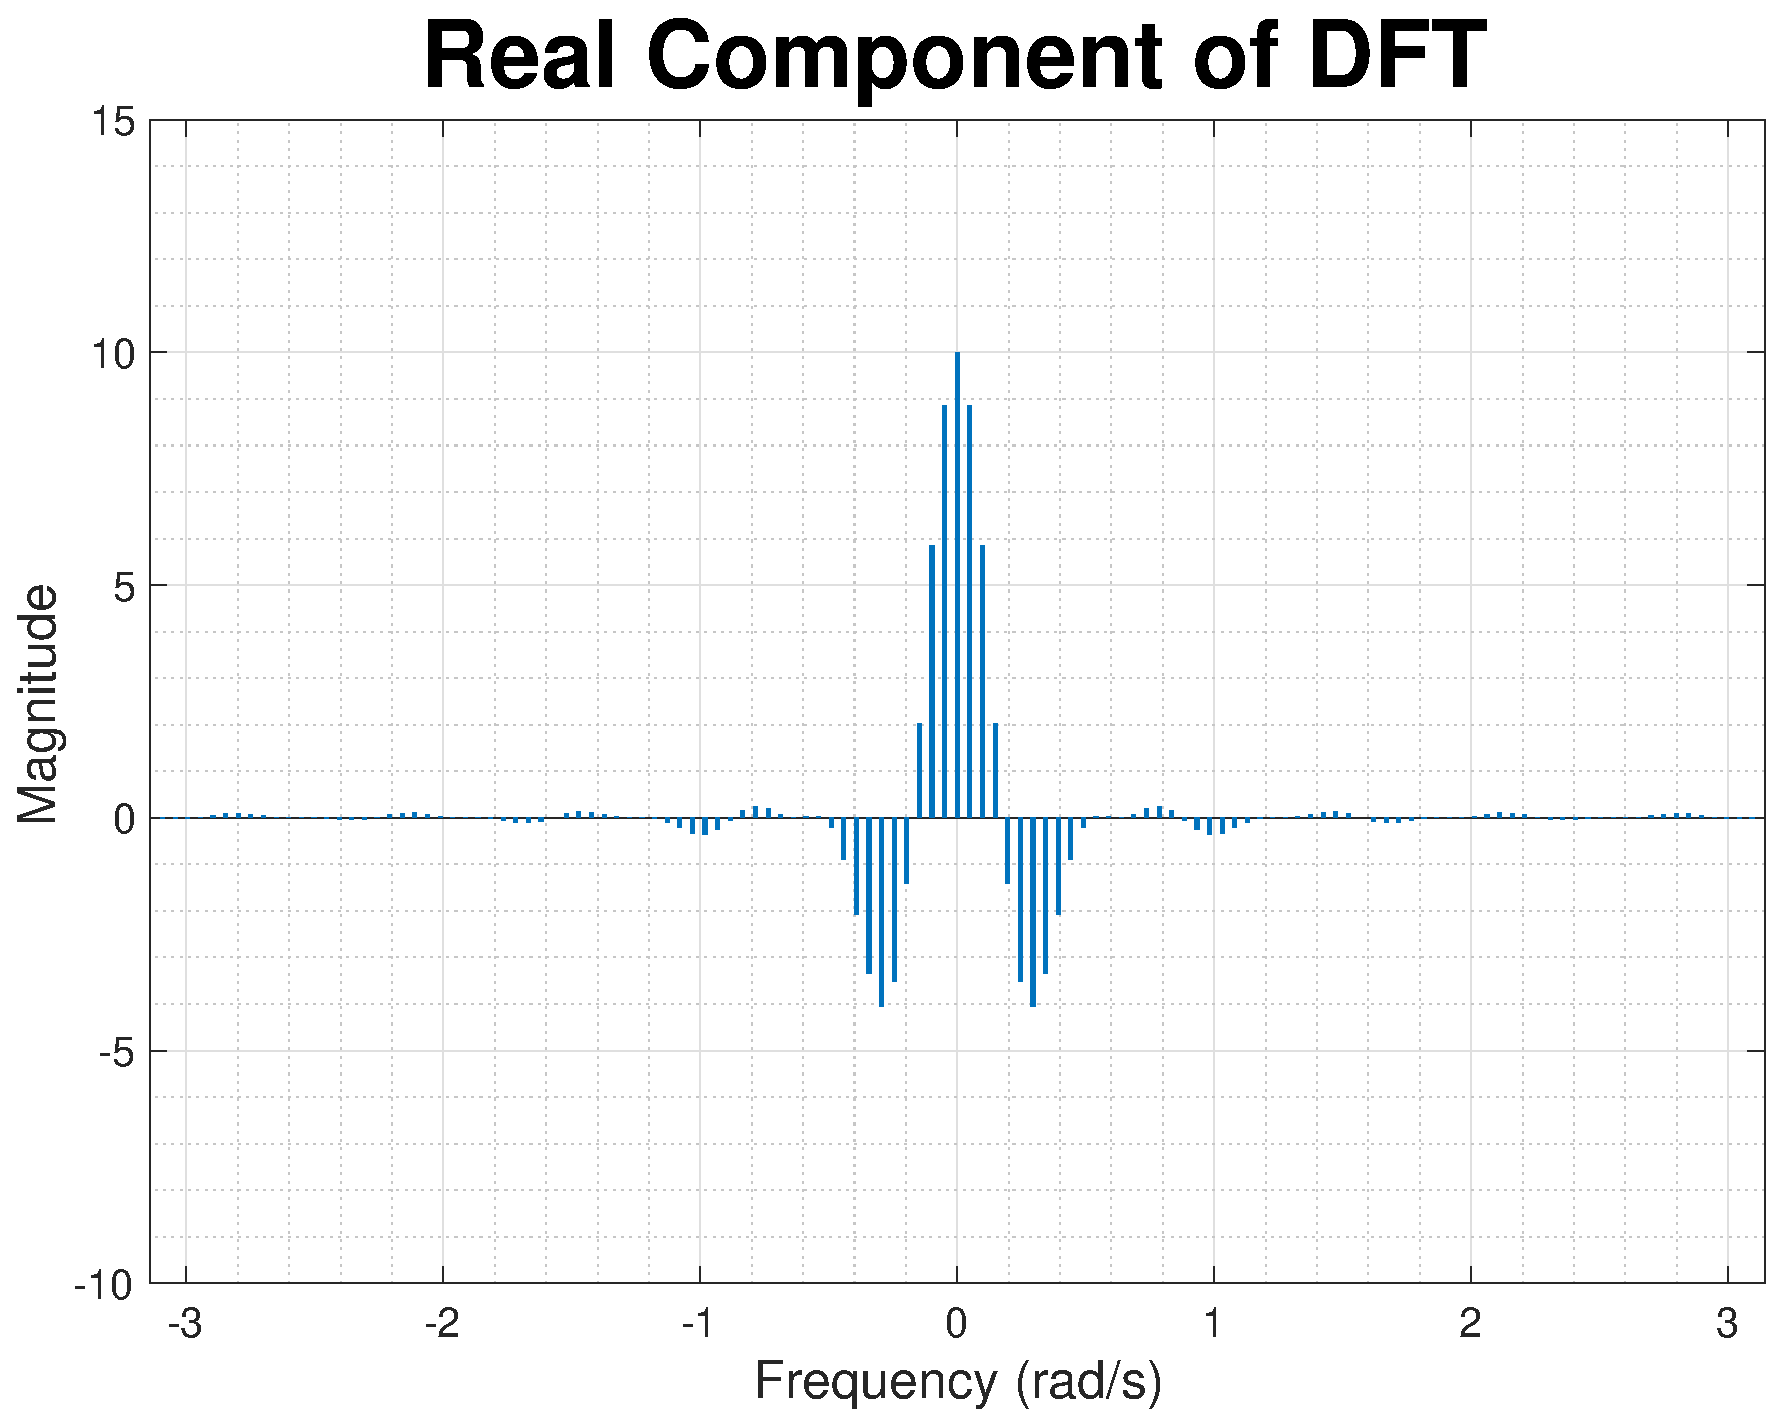
\includegraphics[width=0.49\textwidth]{part1/dft_spectra_acf_z_real}
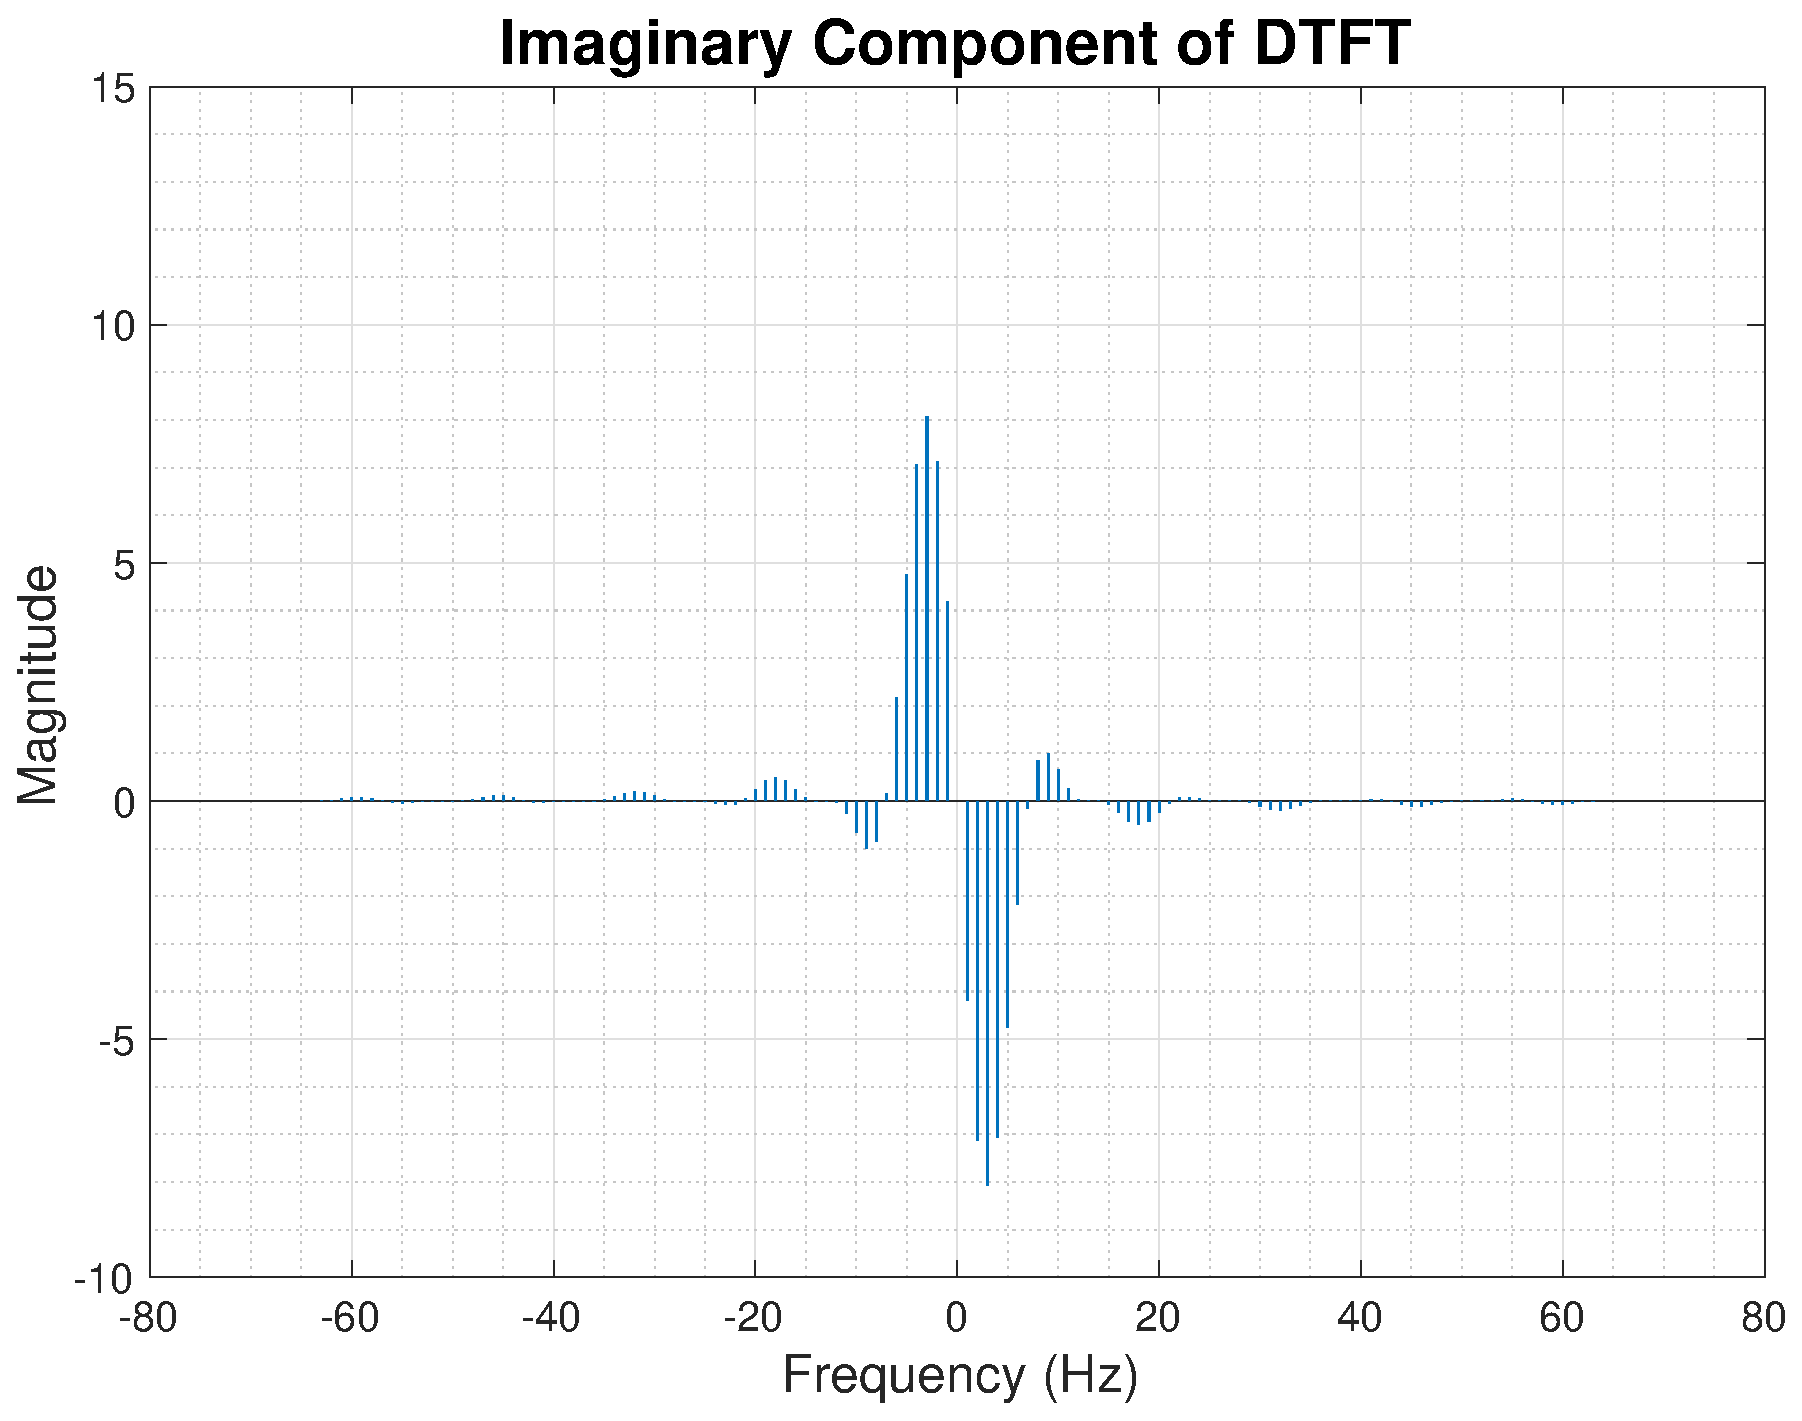
\includegraphics[width=0.49\textwidth]{part1/dft_spectra_acf_z_imag}
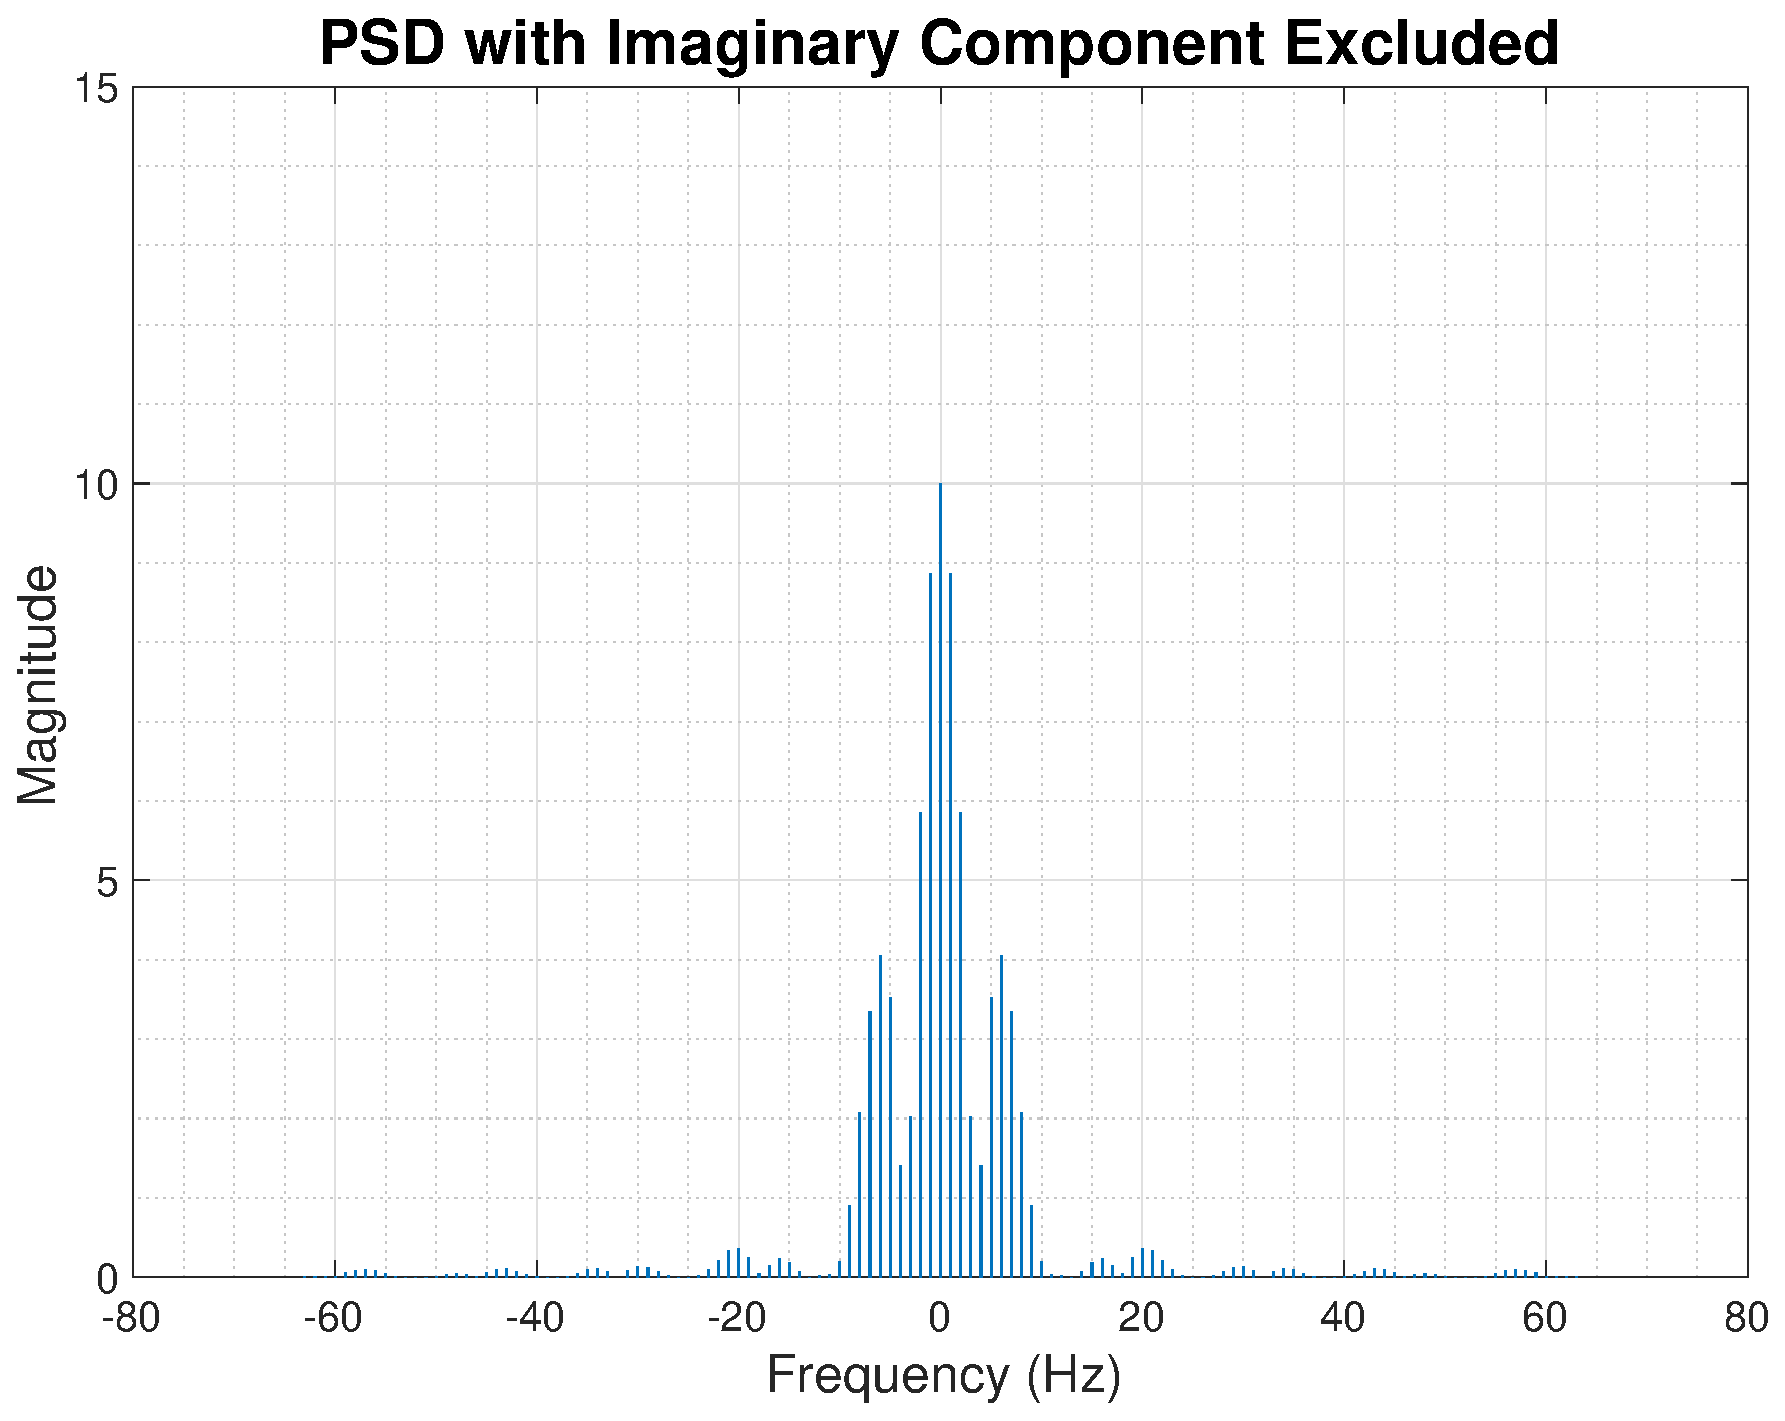
\includegraphics[width=0.49\textwidth]{part1/acf_z_psd_without_imag}
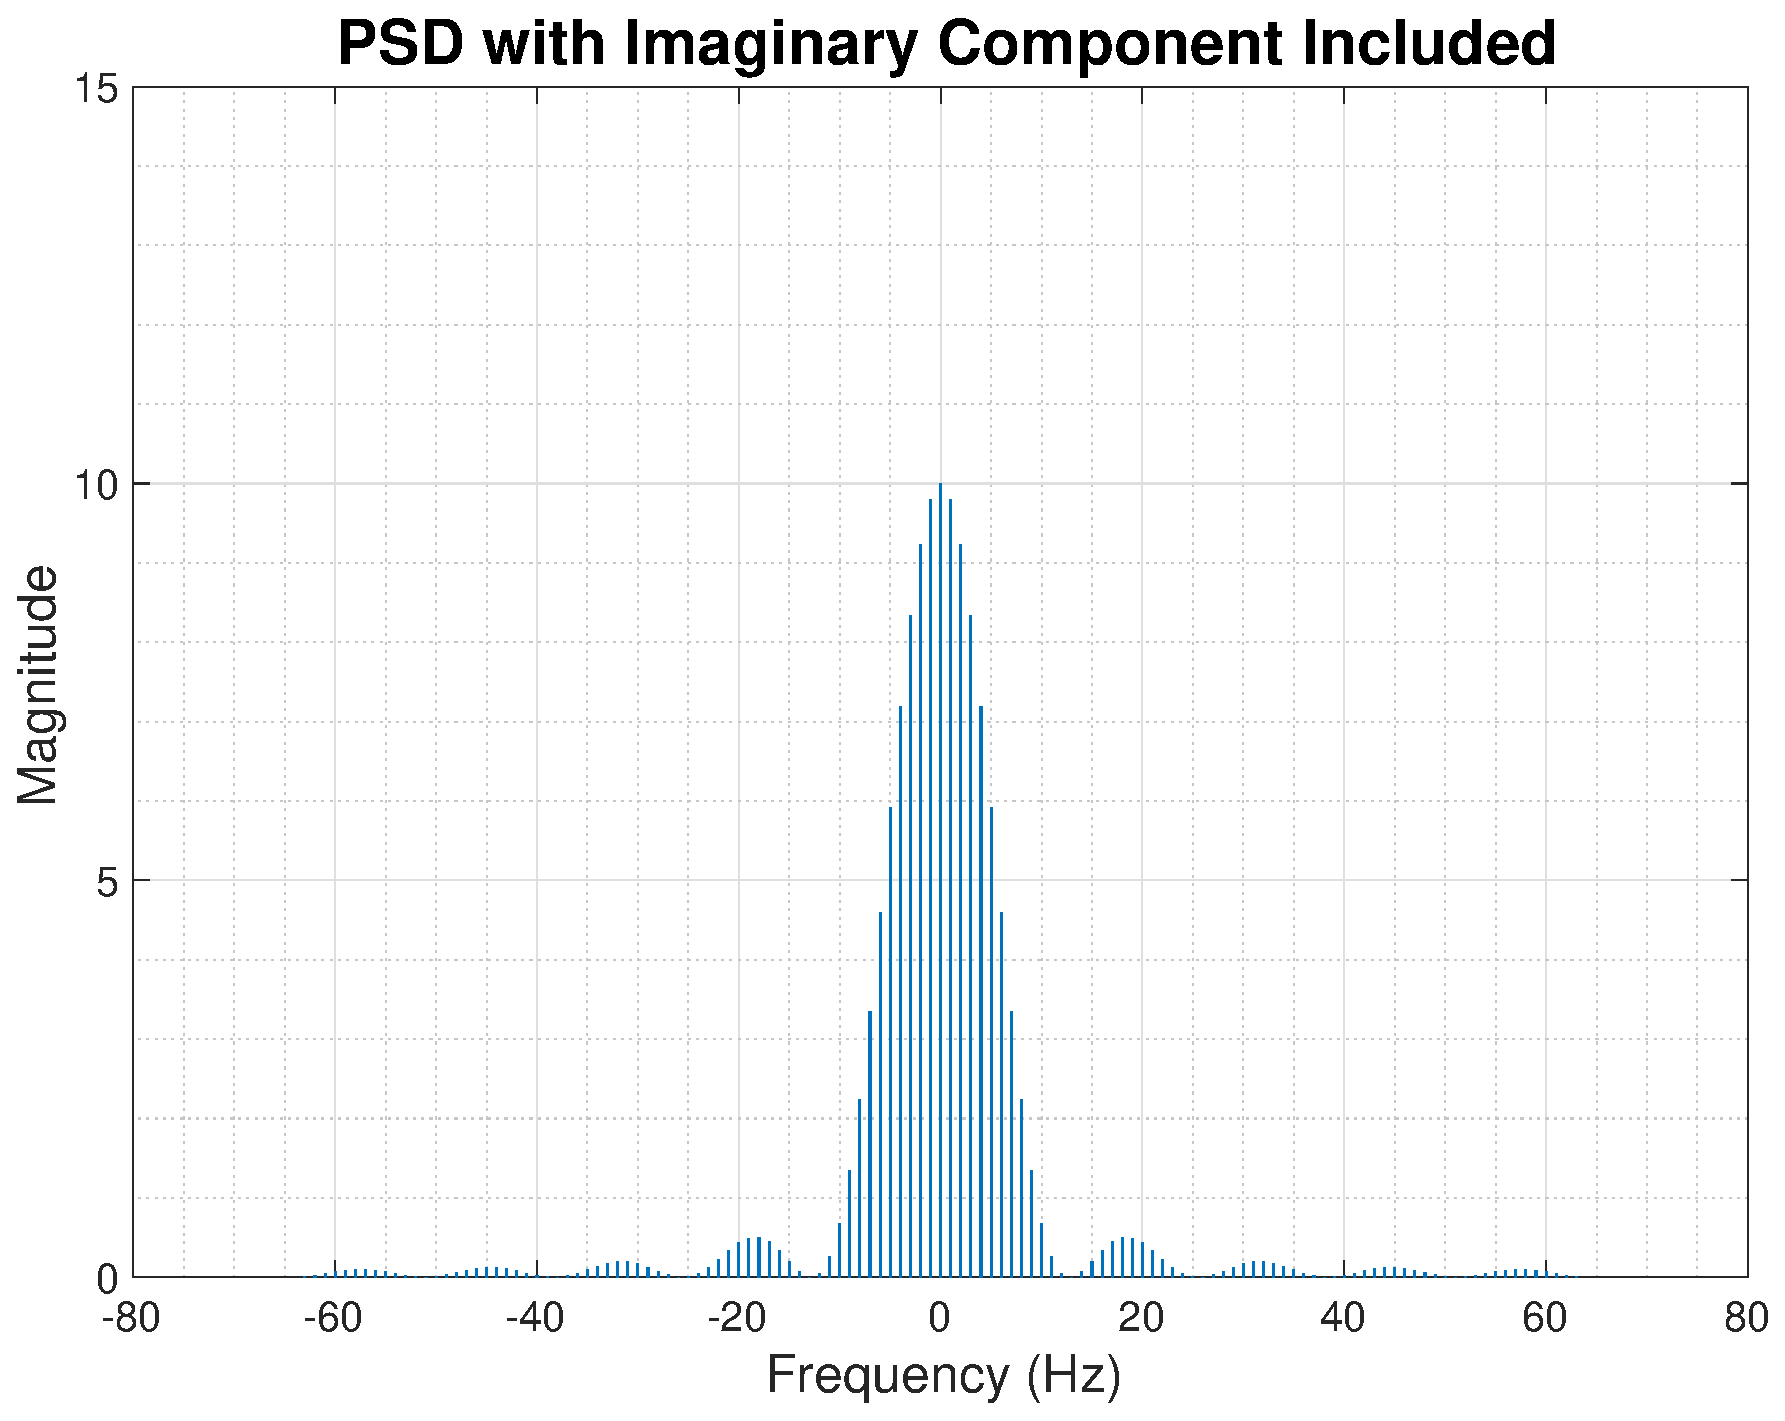
\includegraphics[width=0.49\textwidth]{part1/acf_z_psd_with_imag}
\caption{Random Caption}
\end{figure}

\subsection{Resolution and Leakage of Periodogram-based Methods}


\begin{figure}[H]
\centering{}
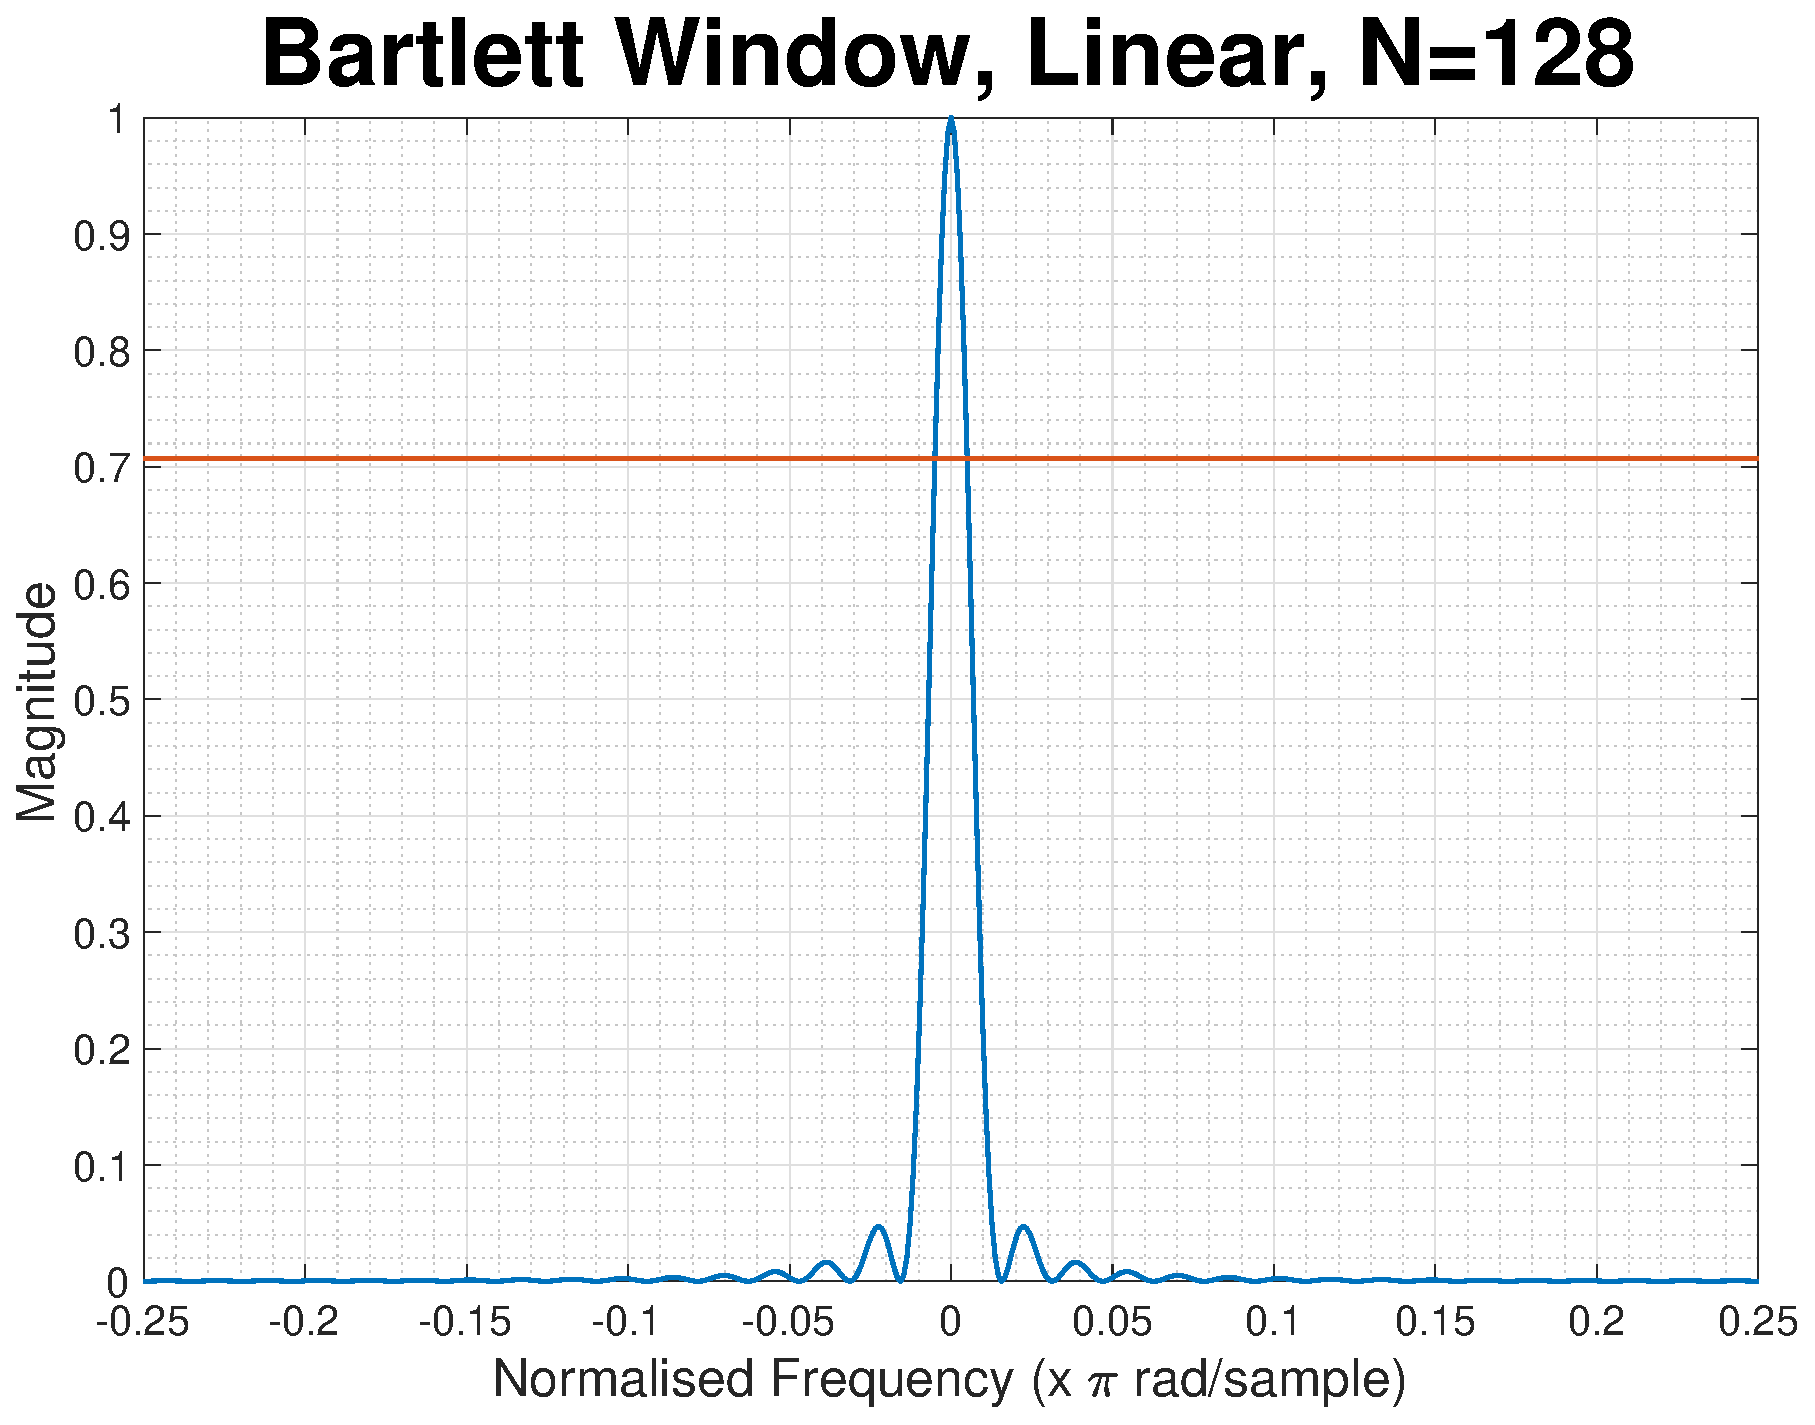
\includegraphics[width=0.49\textwidth]{part1/bartlett_window_N_128_linear}
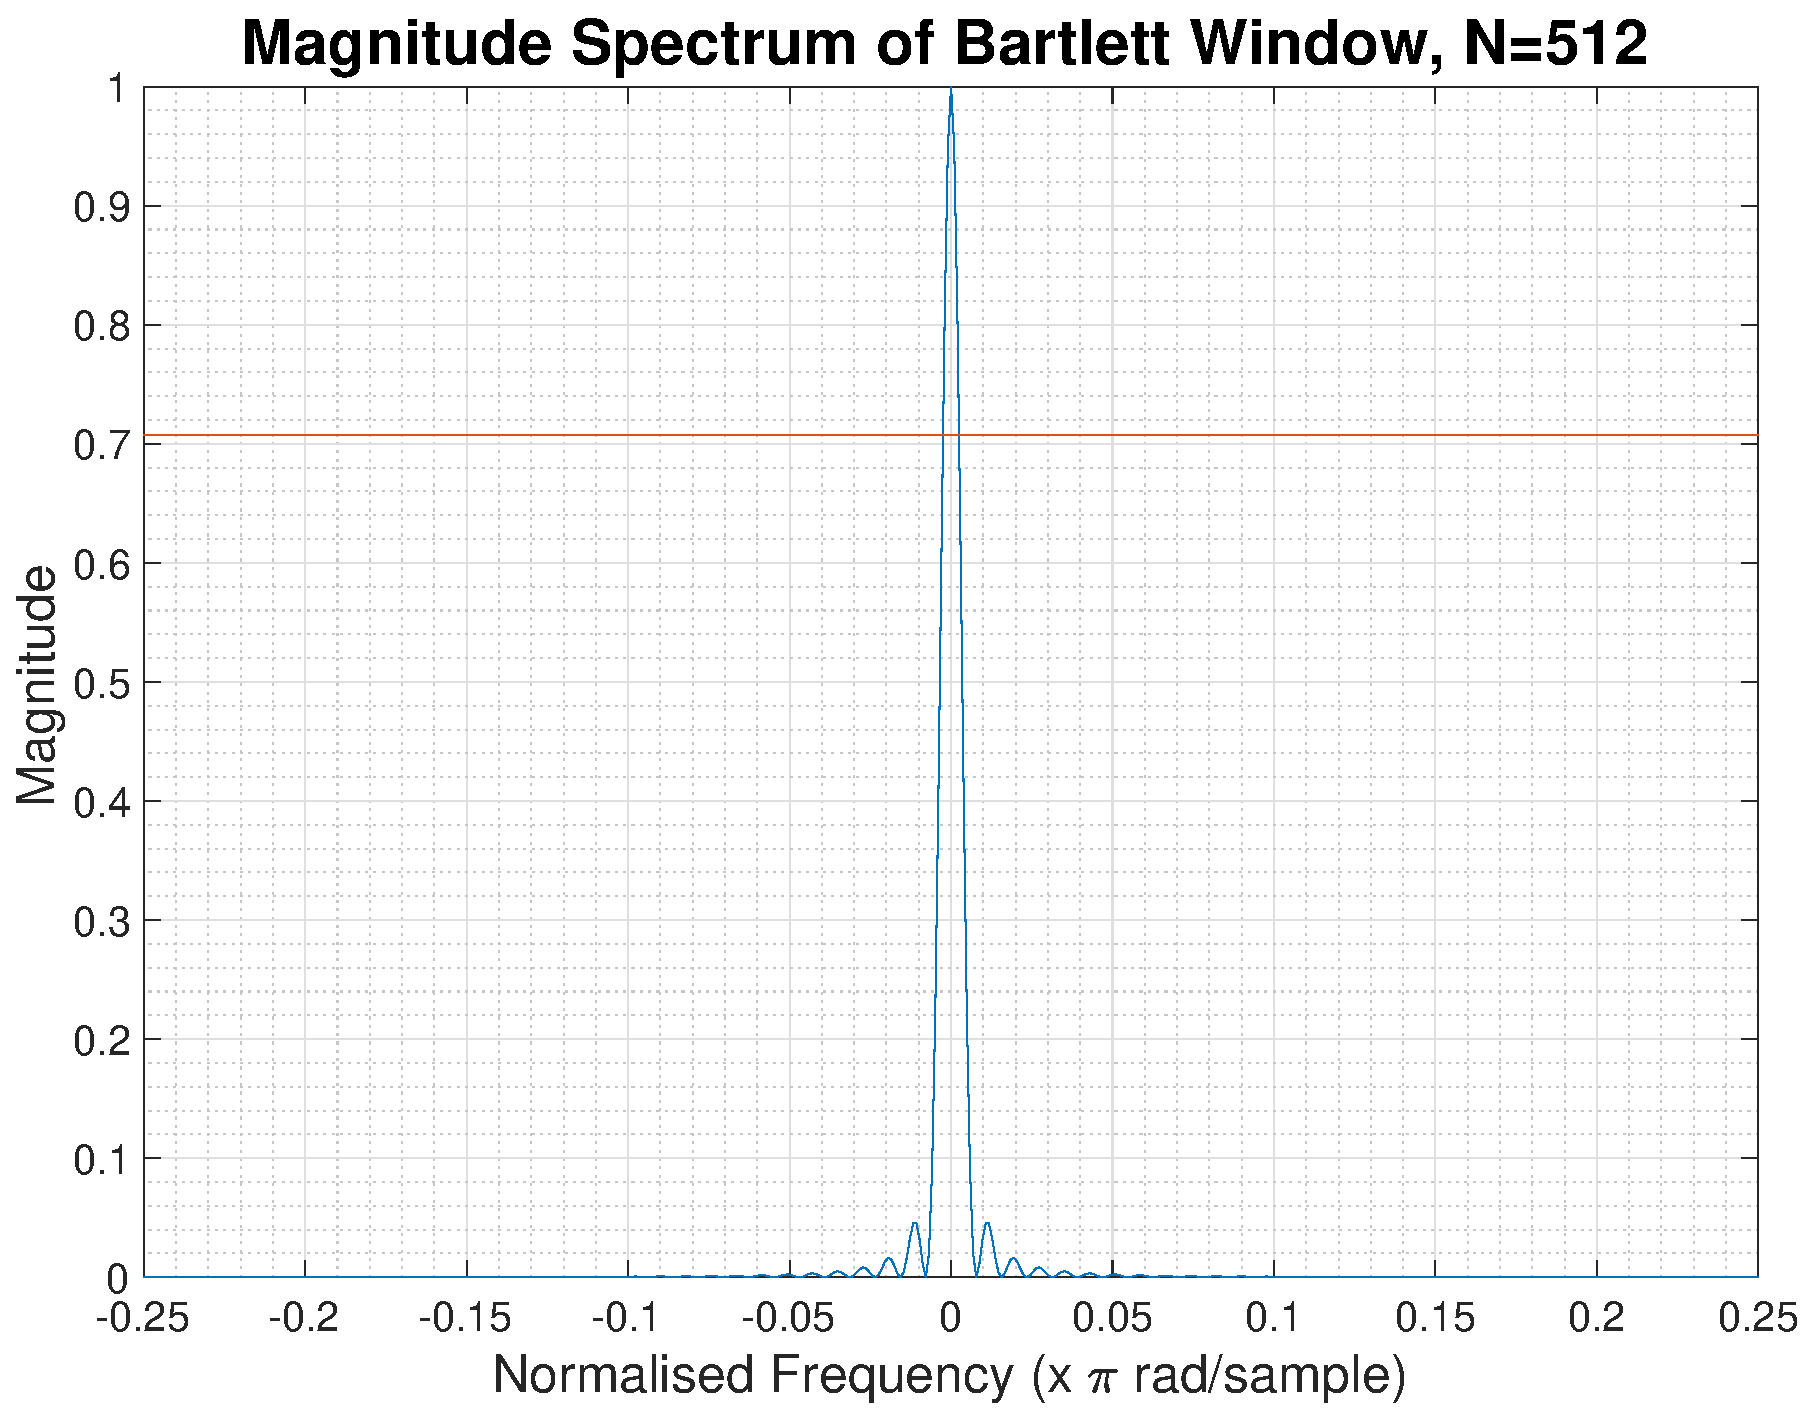
\includegraphics[width=0.49\textwidth]{part1/bartlett_window_N_512_linear}
\caption{Random Caption}
\end{figure}

\begin{figure}[H]
\centering{}
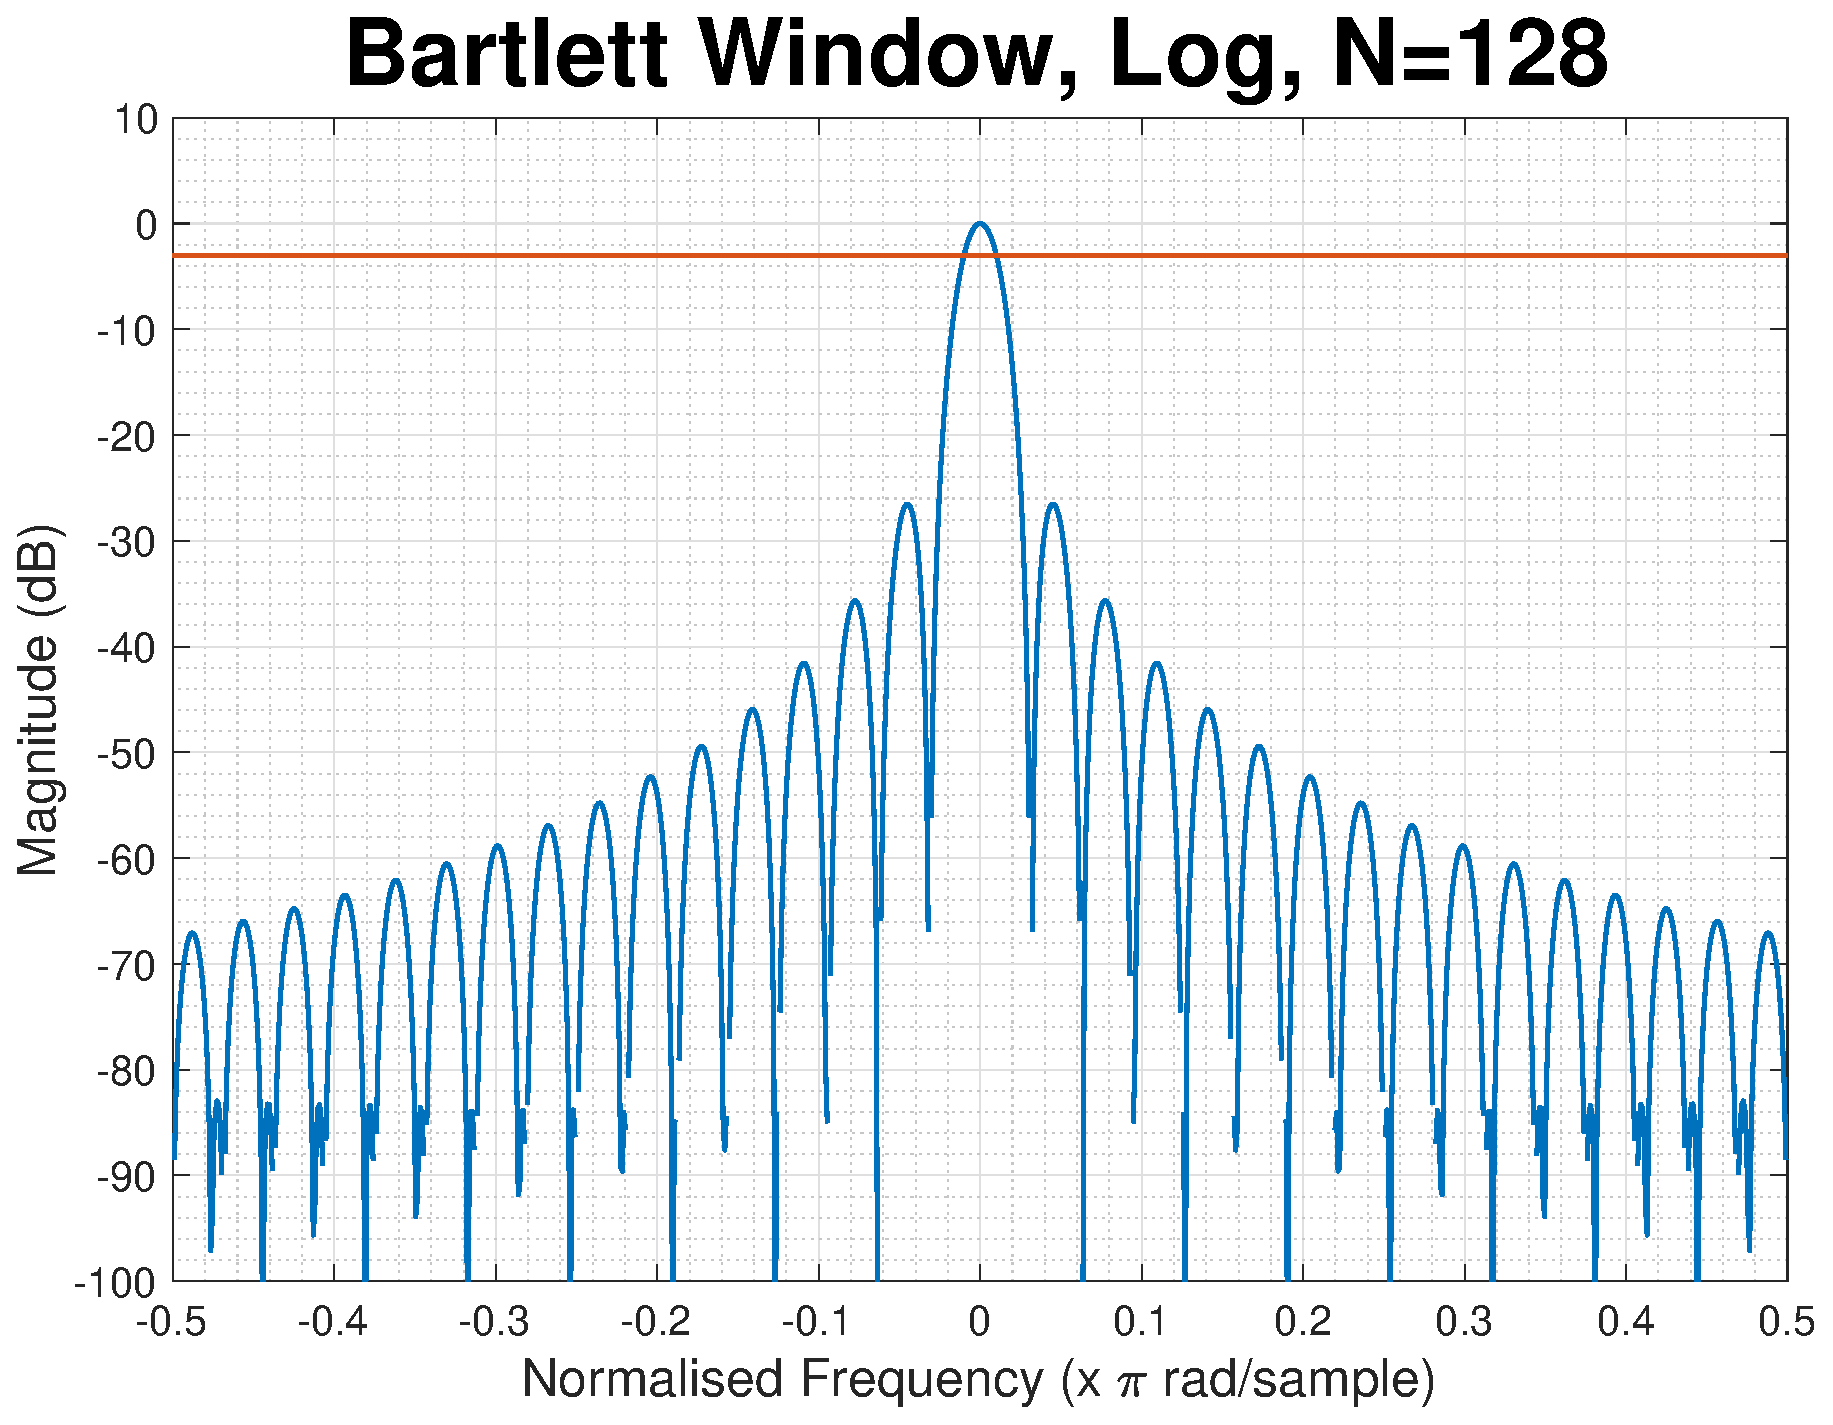
\includegraphics[width=0.49\textwidth]{part1/bartlett_window_N_128_dB}
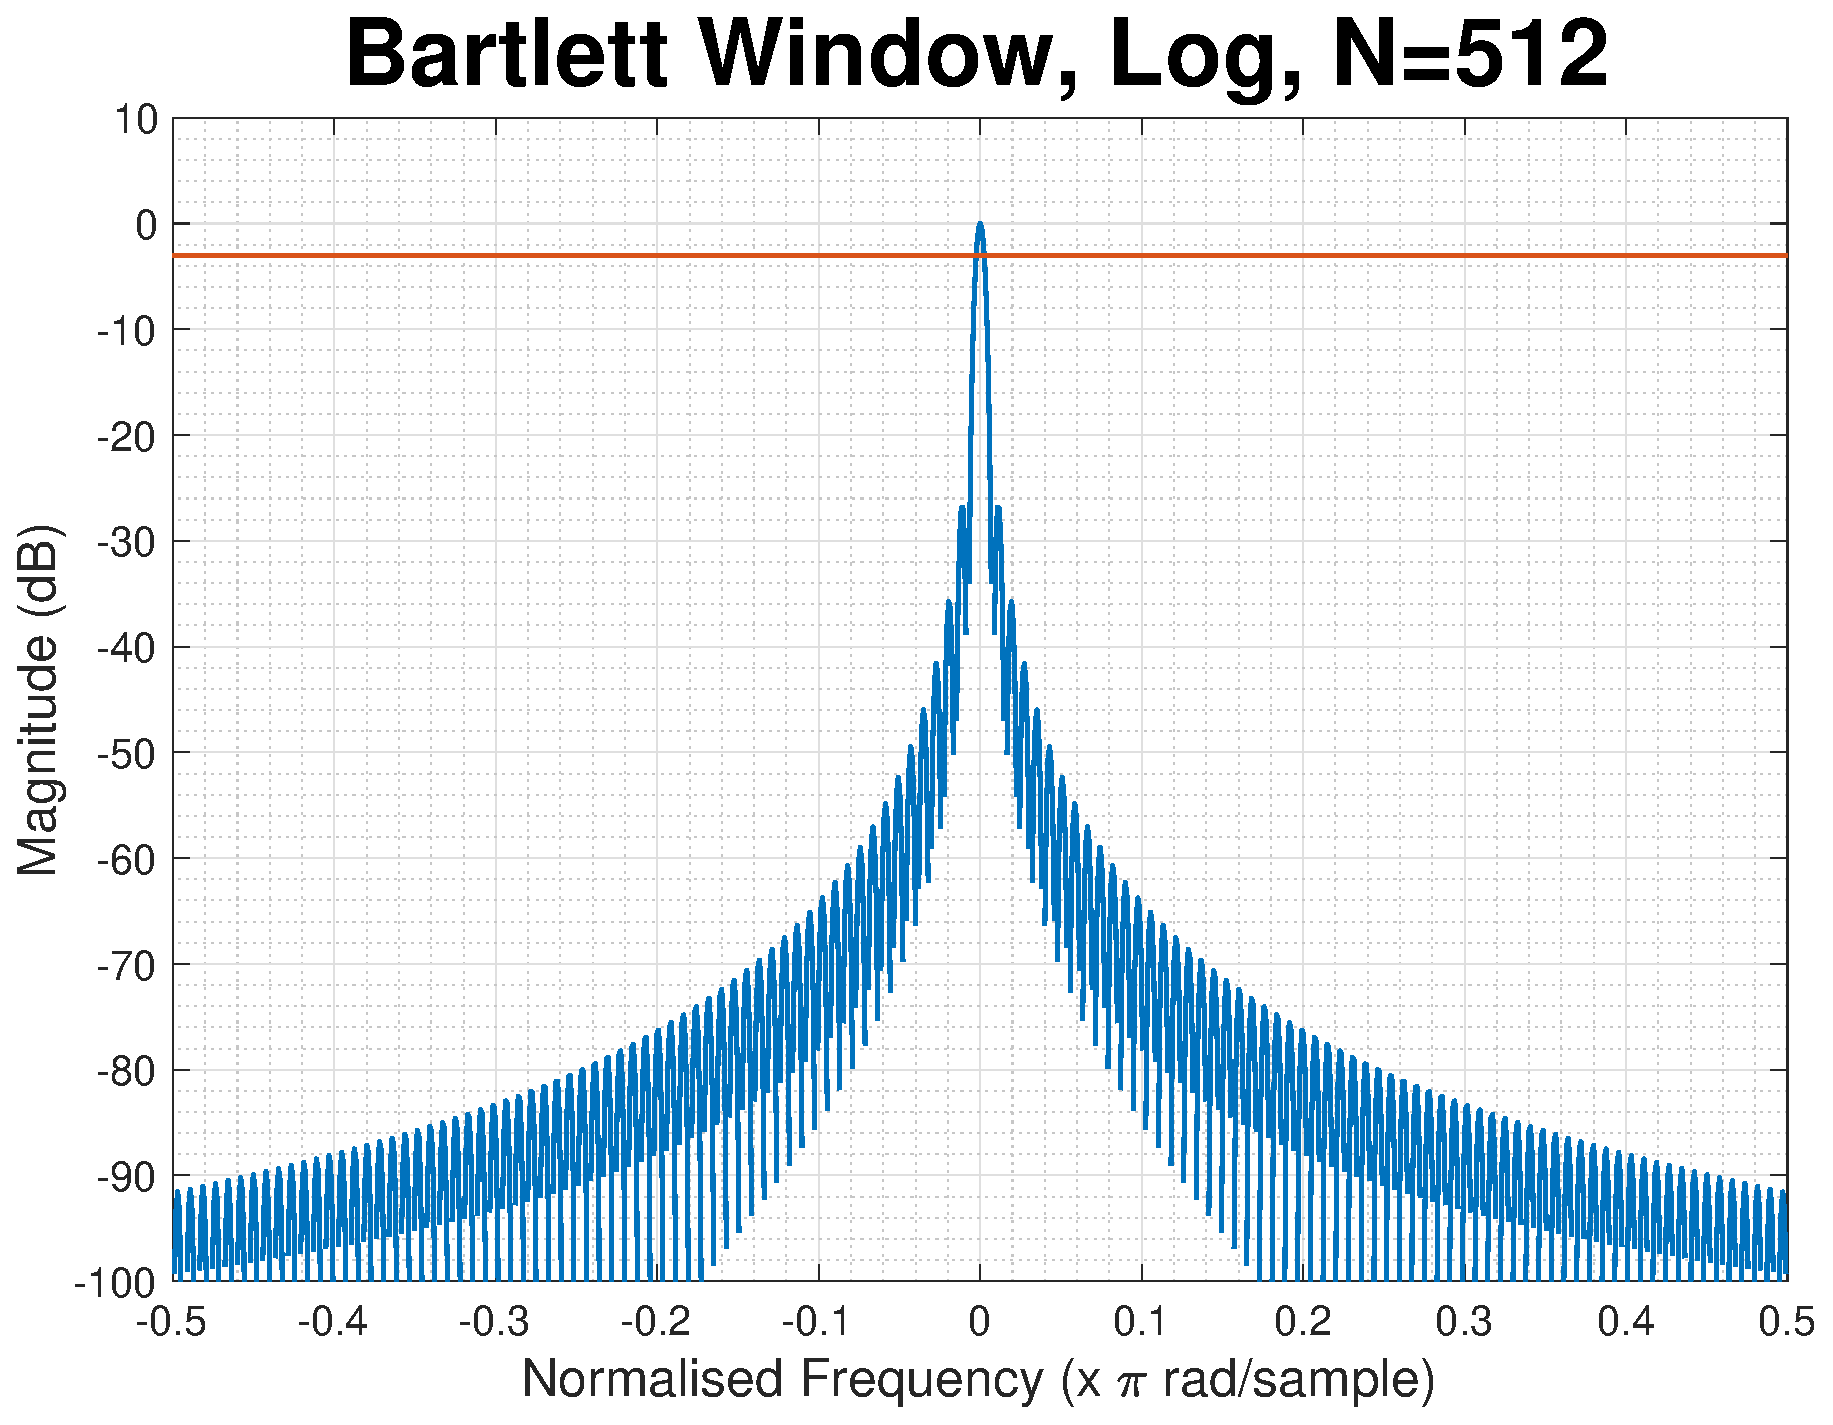
\includegraphics[width=0.49\textwidth]{part1/bartlett_window_N_512_dB}
\caption{Random Caption}
\end{figure}

\begin{figure}[H]
\centering{}
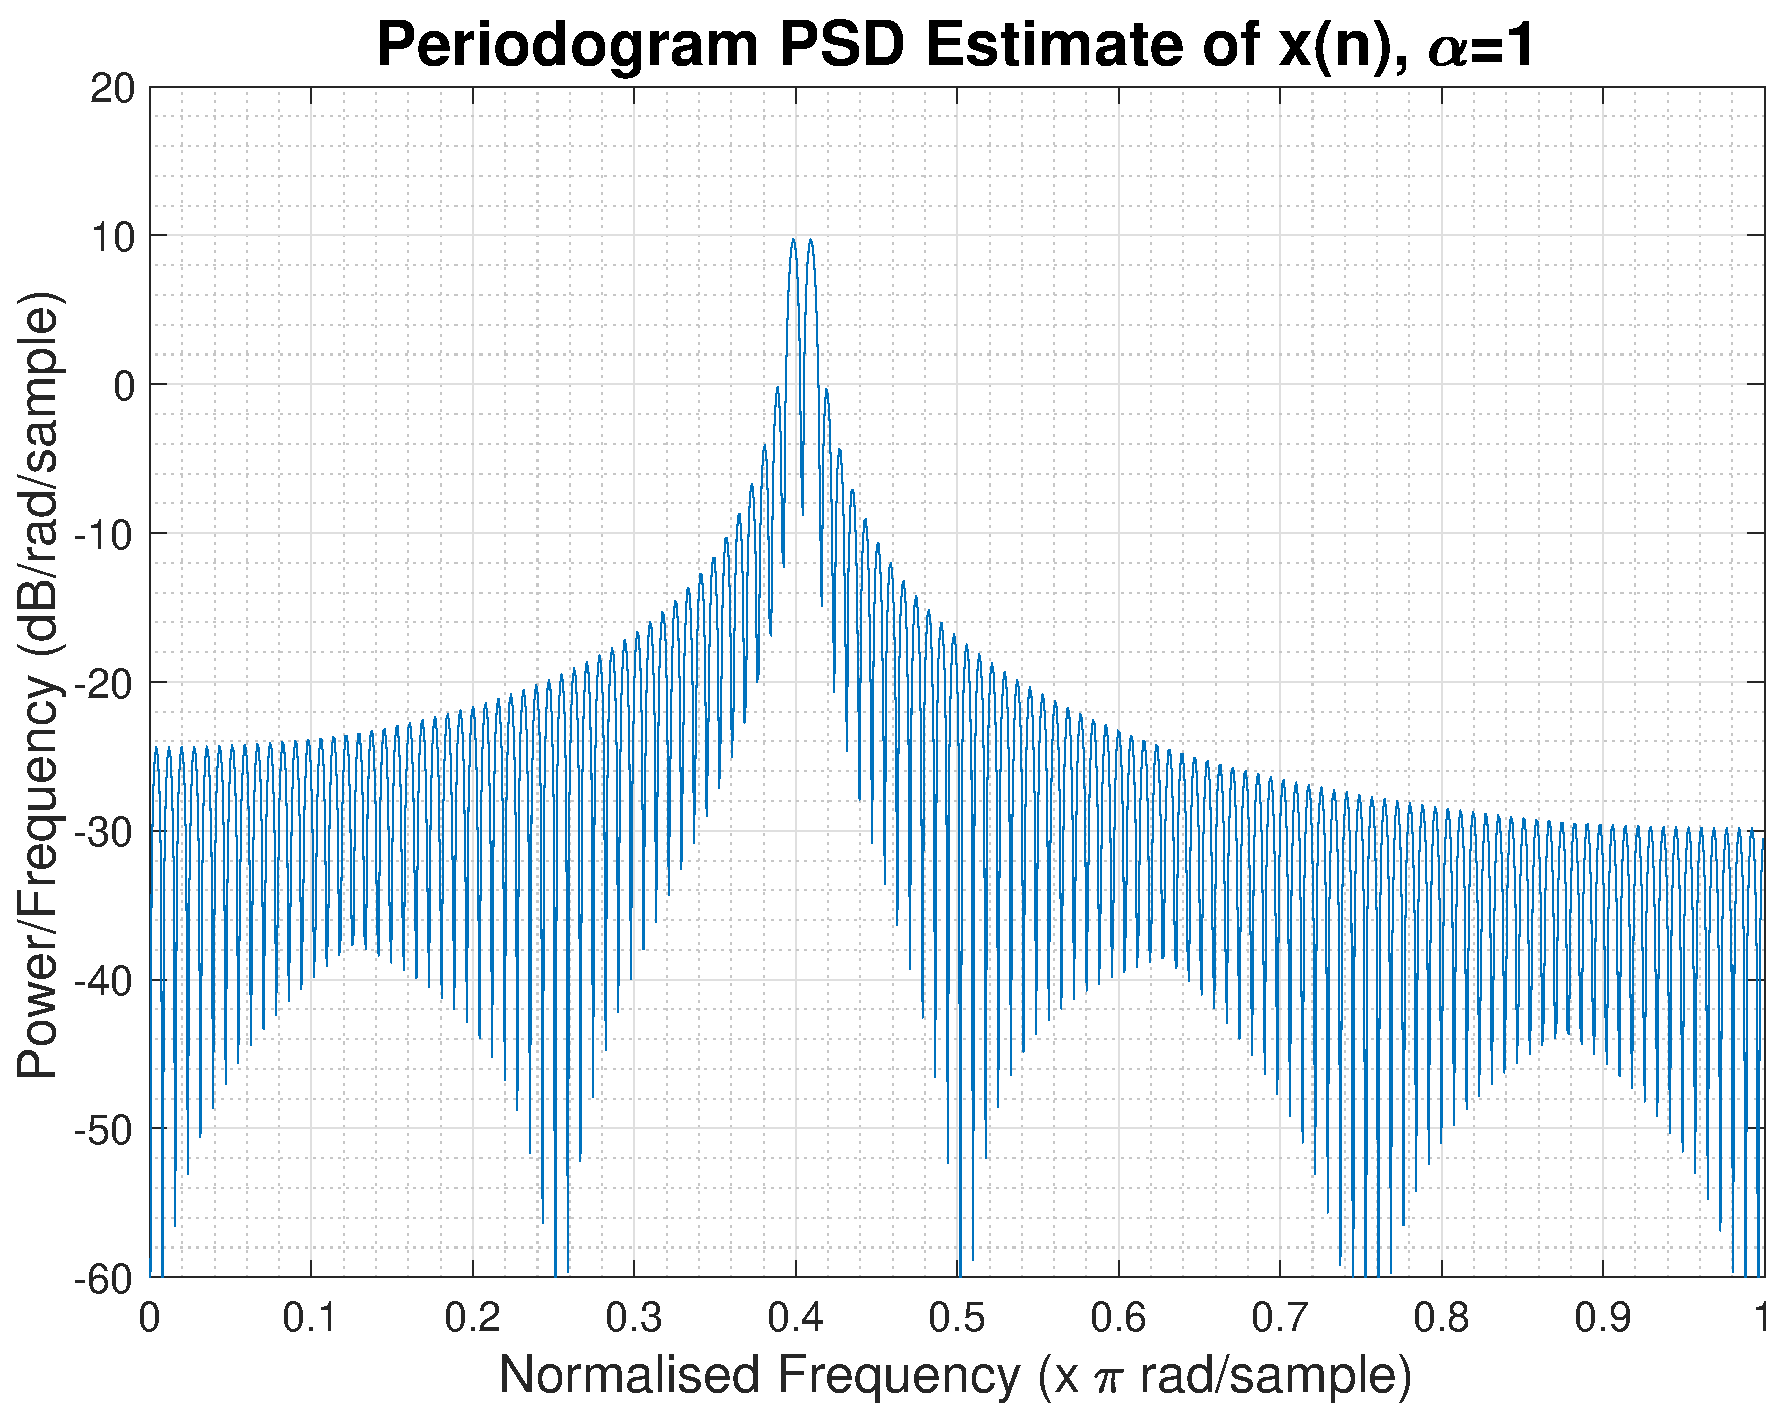
\includegraphics[width=0.49\textwidth]{part1/periodogram_xn_alpha_1}
\caption{Random Caption}
\end{figure}

\begin{figure}[H]
\centering{}
\includegraphics[width=0.49\textwidth]{part1/periodogram_xn_alpha_point_65}
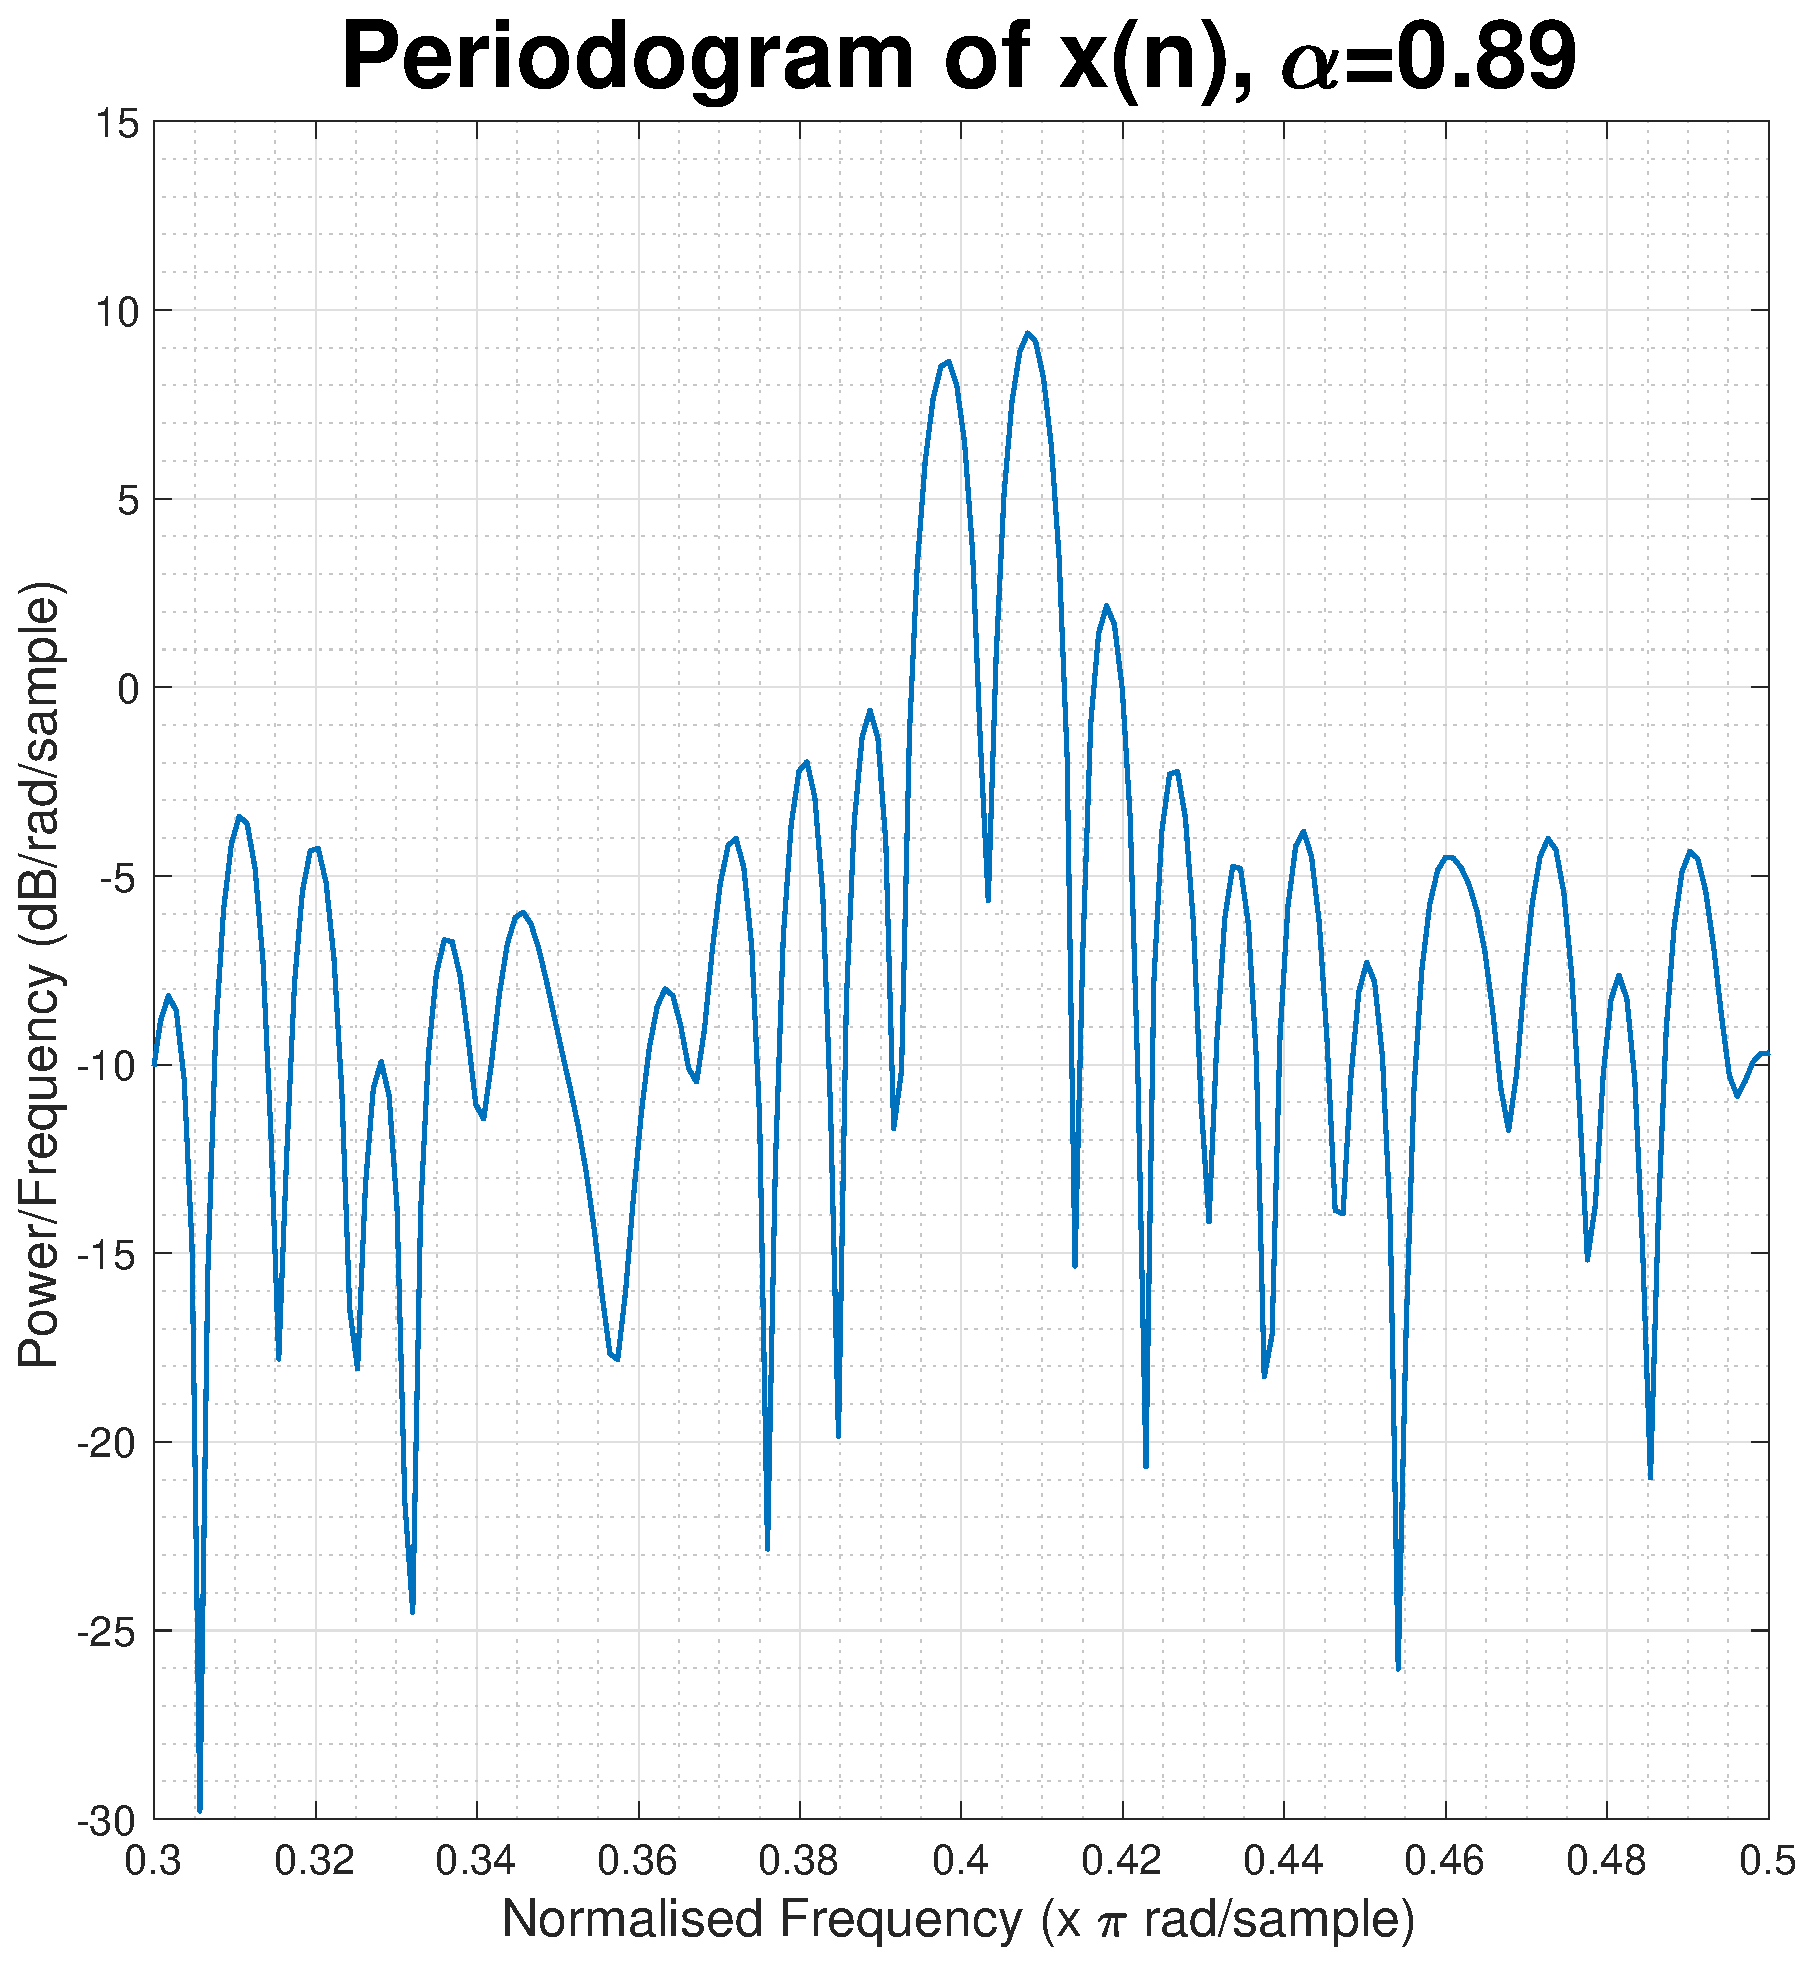
\includegraphics[width=0.49\textwidth]{part1/periodogram_xn_alpha_point_60}
\caption{Random Caption}
\end{figure}

\begin{figure}[H]
\centering{}
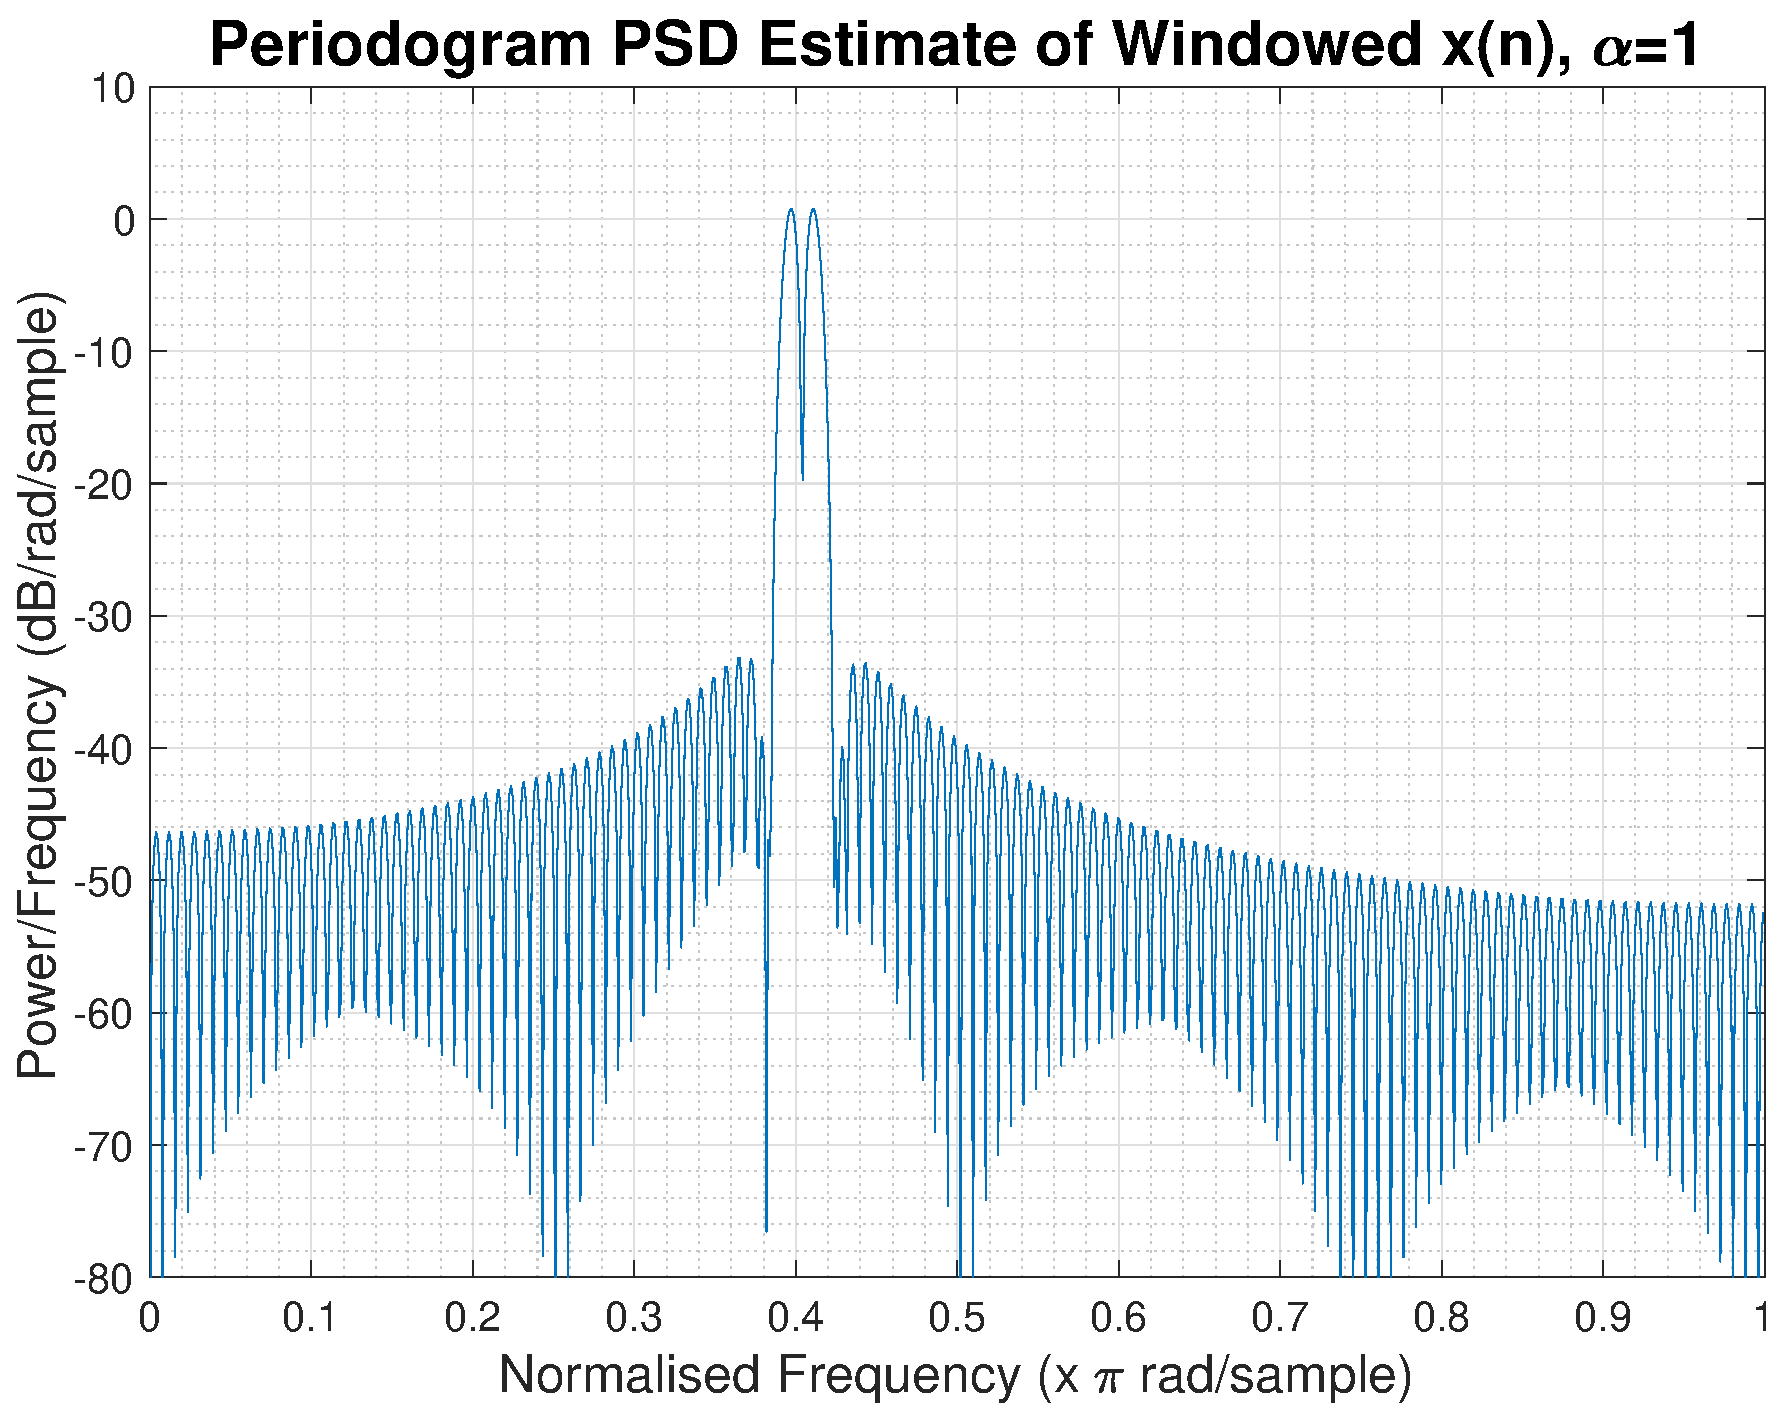
\includegraphics[width=0.49\textwidth]{part1/periodogram_windowed_xn_alpha_1}
\caption{Random Caption}
\end{figure}

\begin{figure}[H]
\centering{}
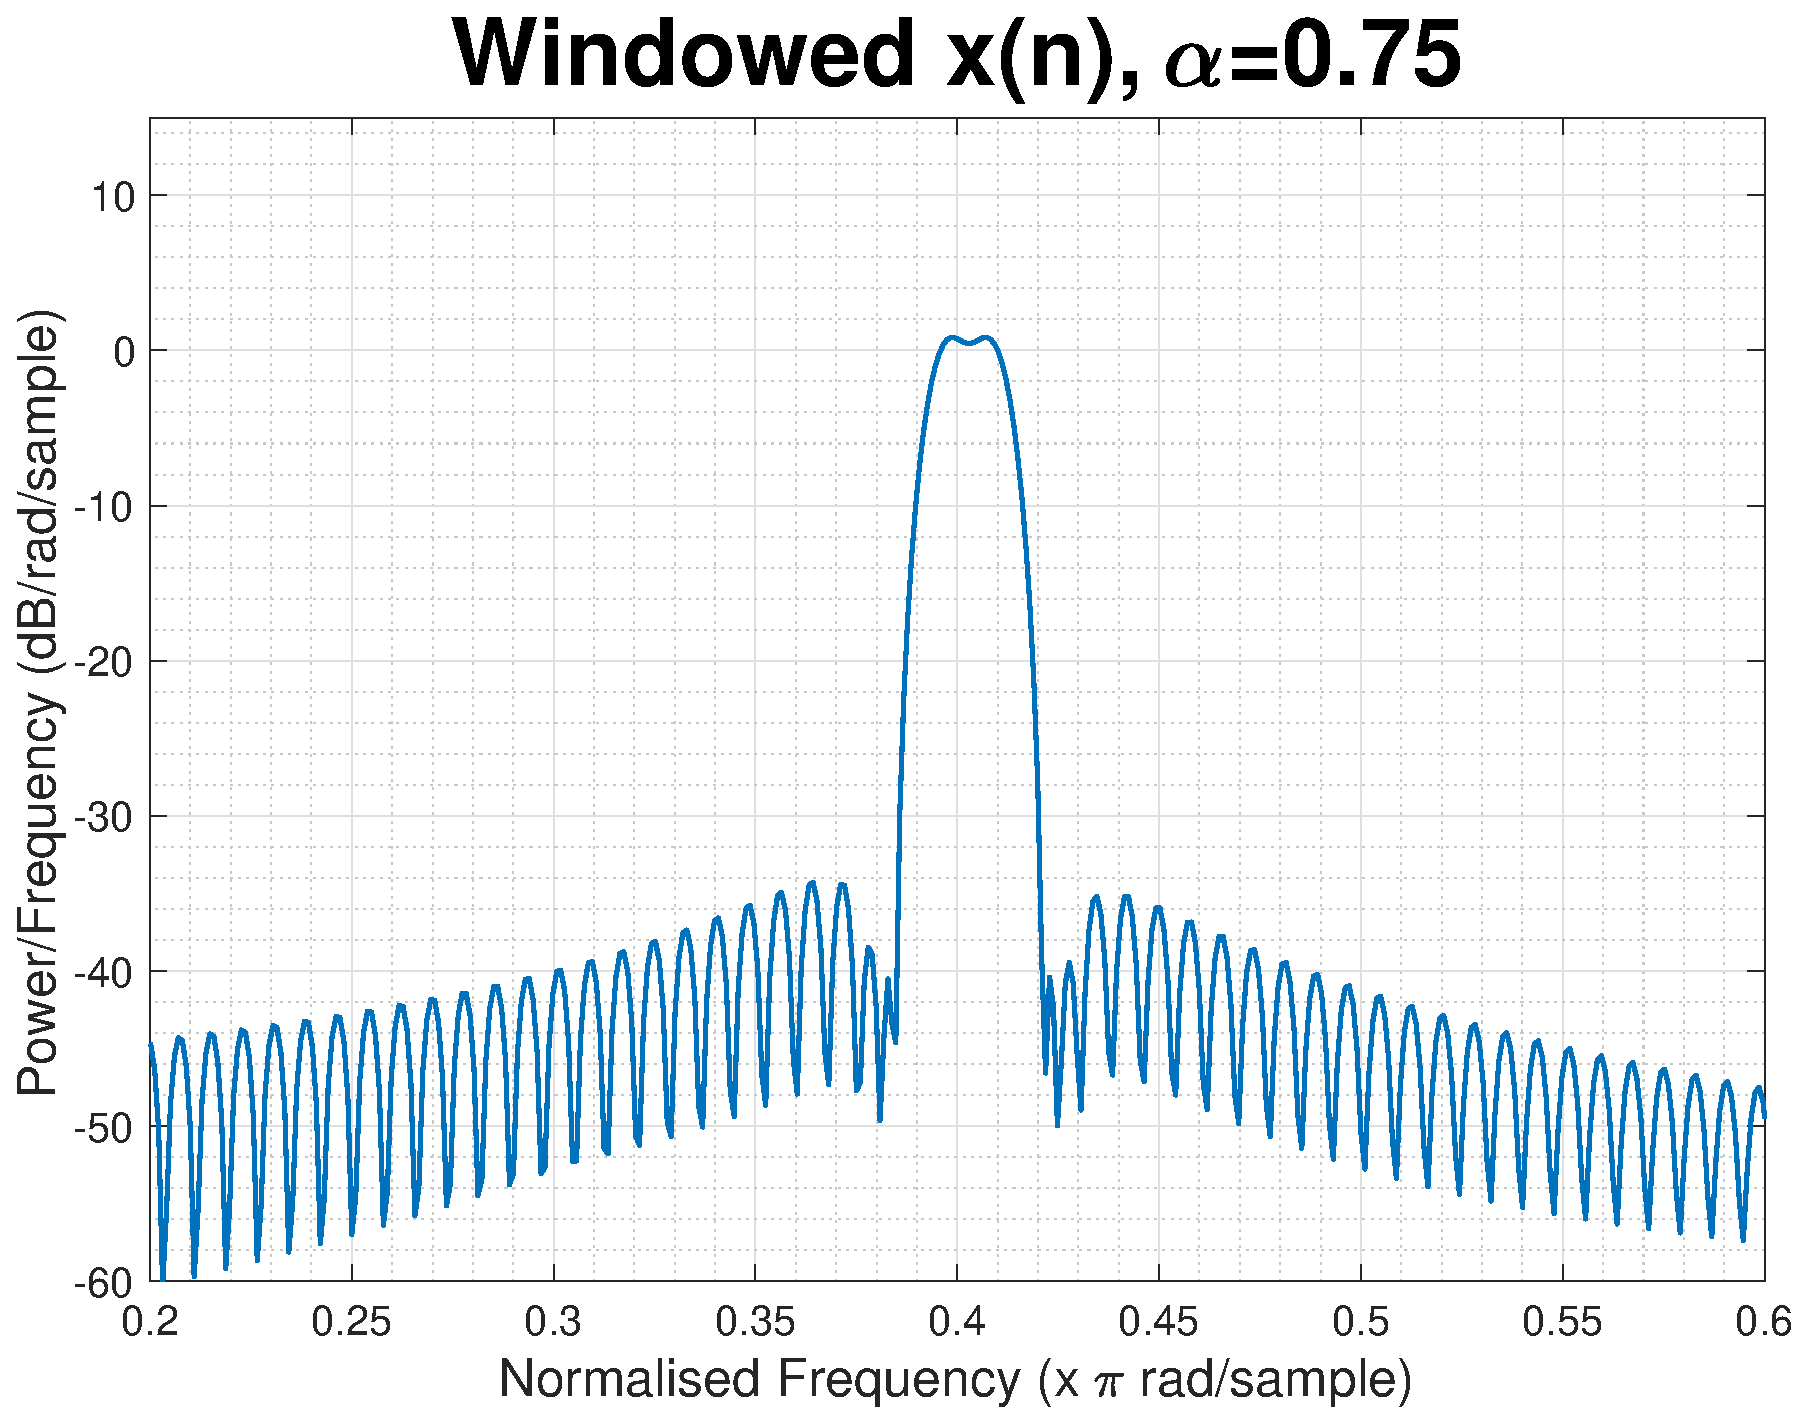
\includegraphics[width=0.49\textwidth]{part1/periodogram_windowed_xn_alpha_point_75}
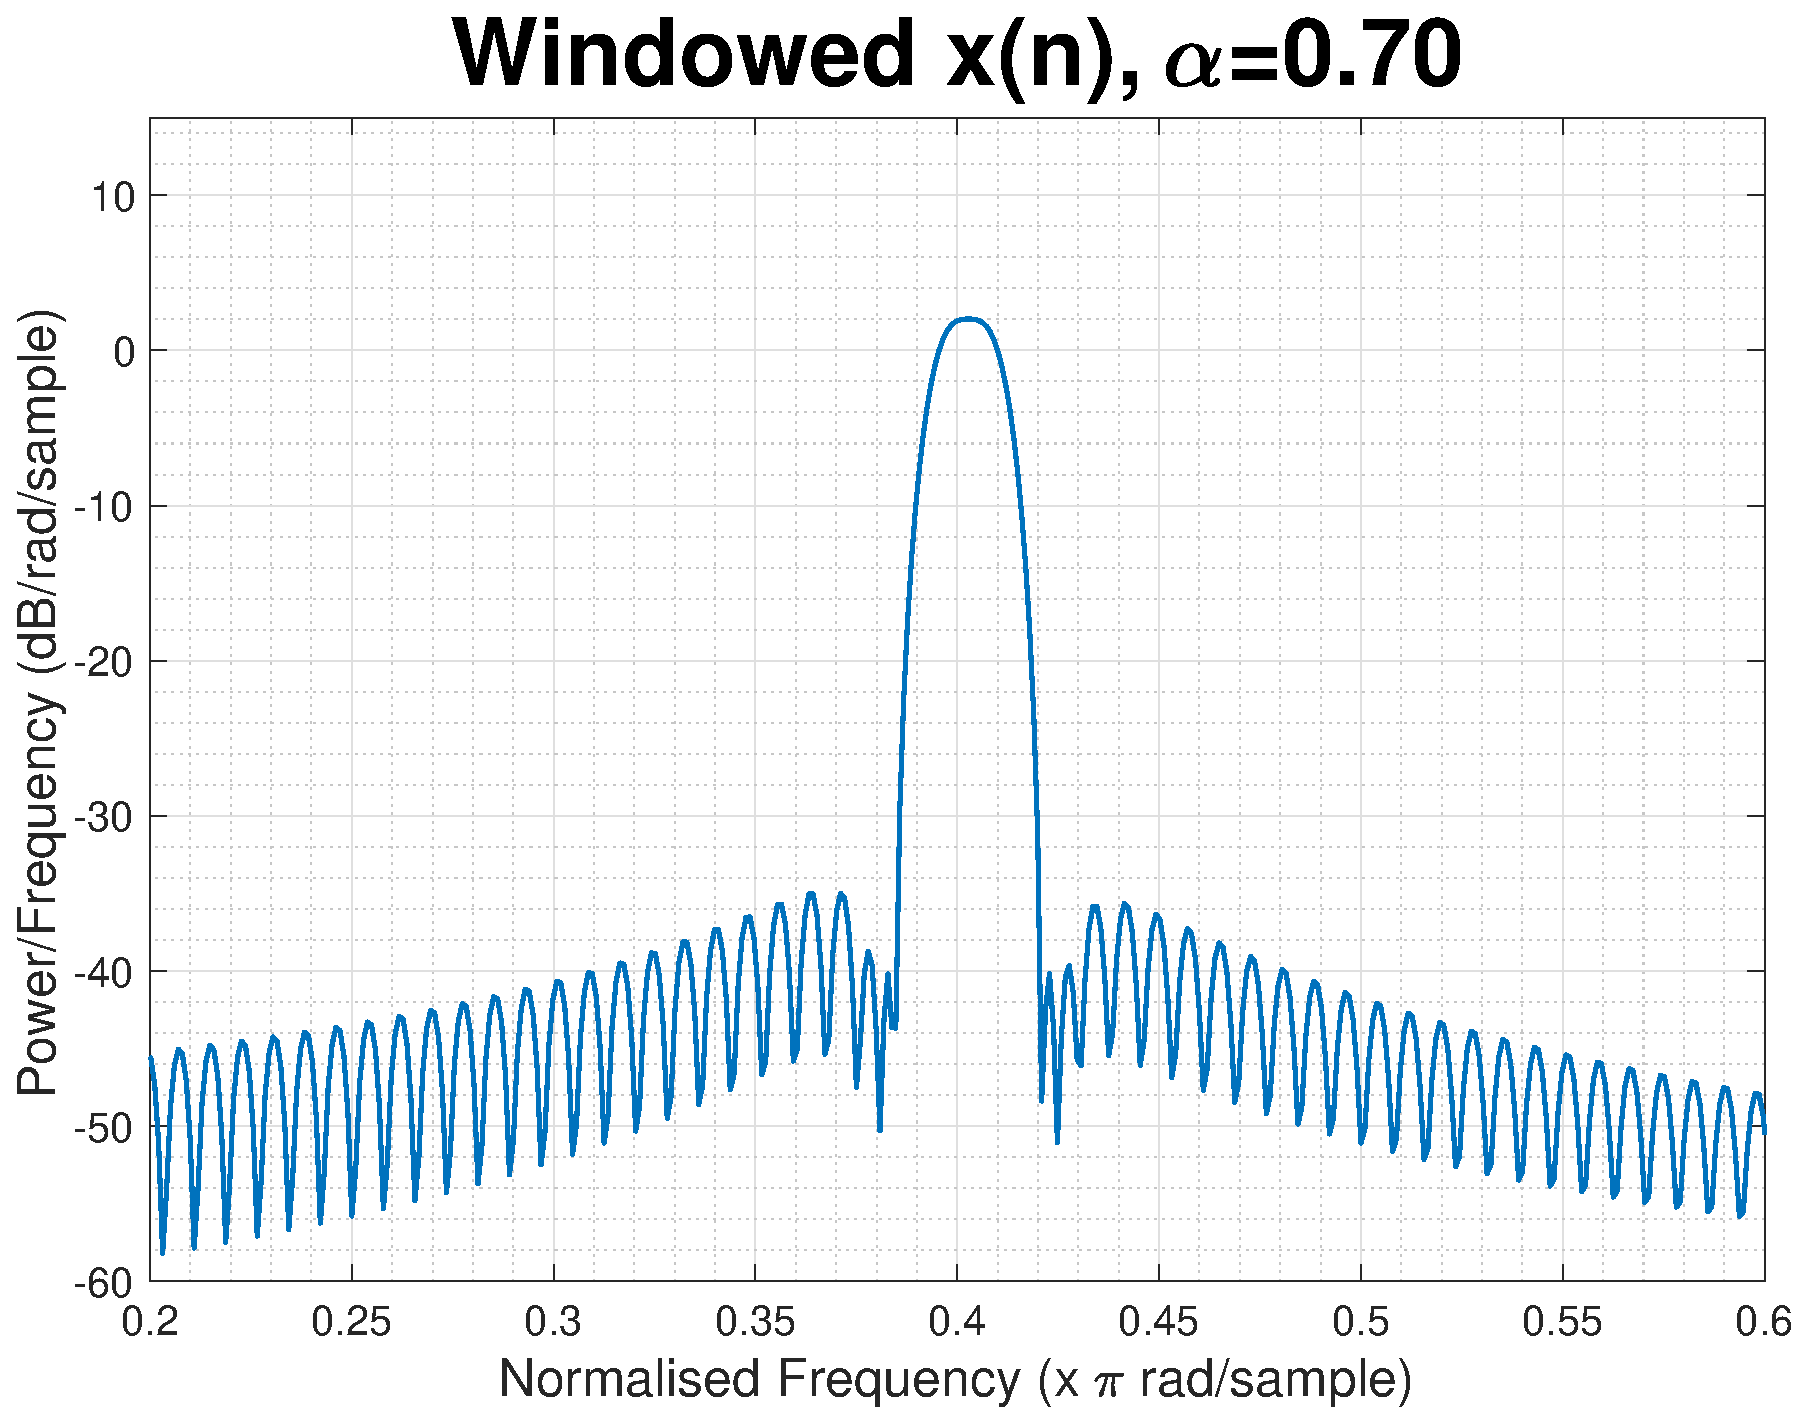
\includegraphics[width=0.49\textwidth]{part1/periodogram_windowed_xn_alpha_point_70}
\caption{Random Caption}
\end{figure}

\begin{figure}[H]
\centering{}
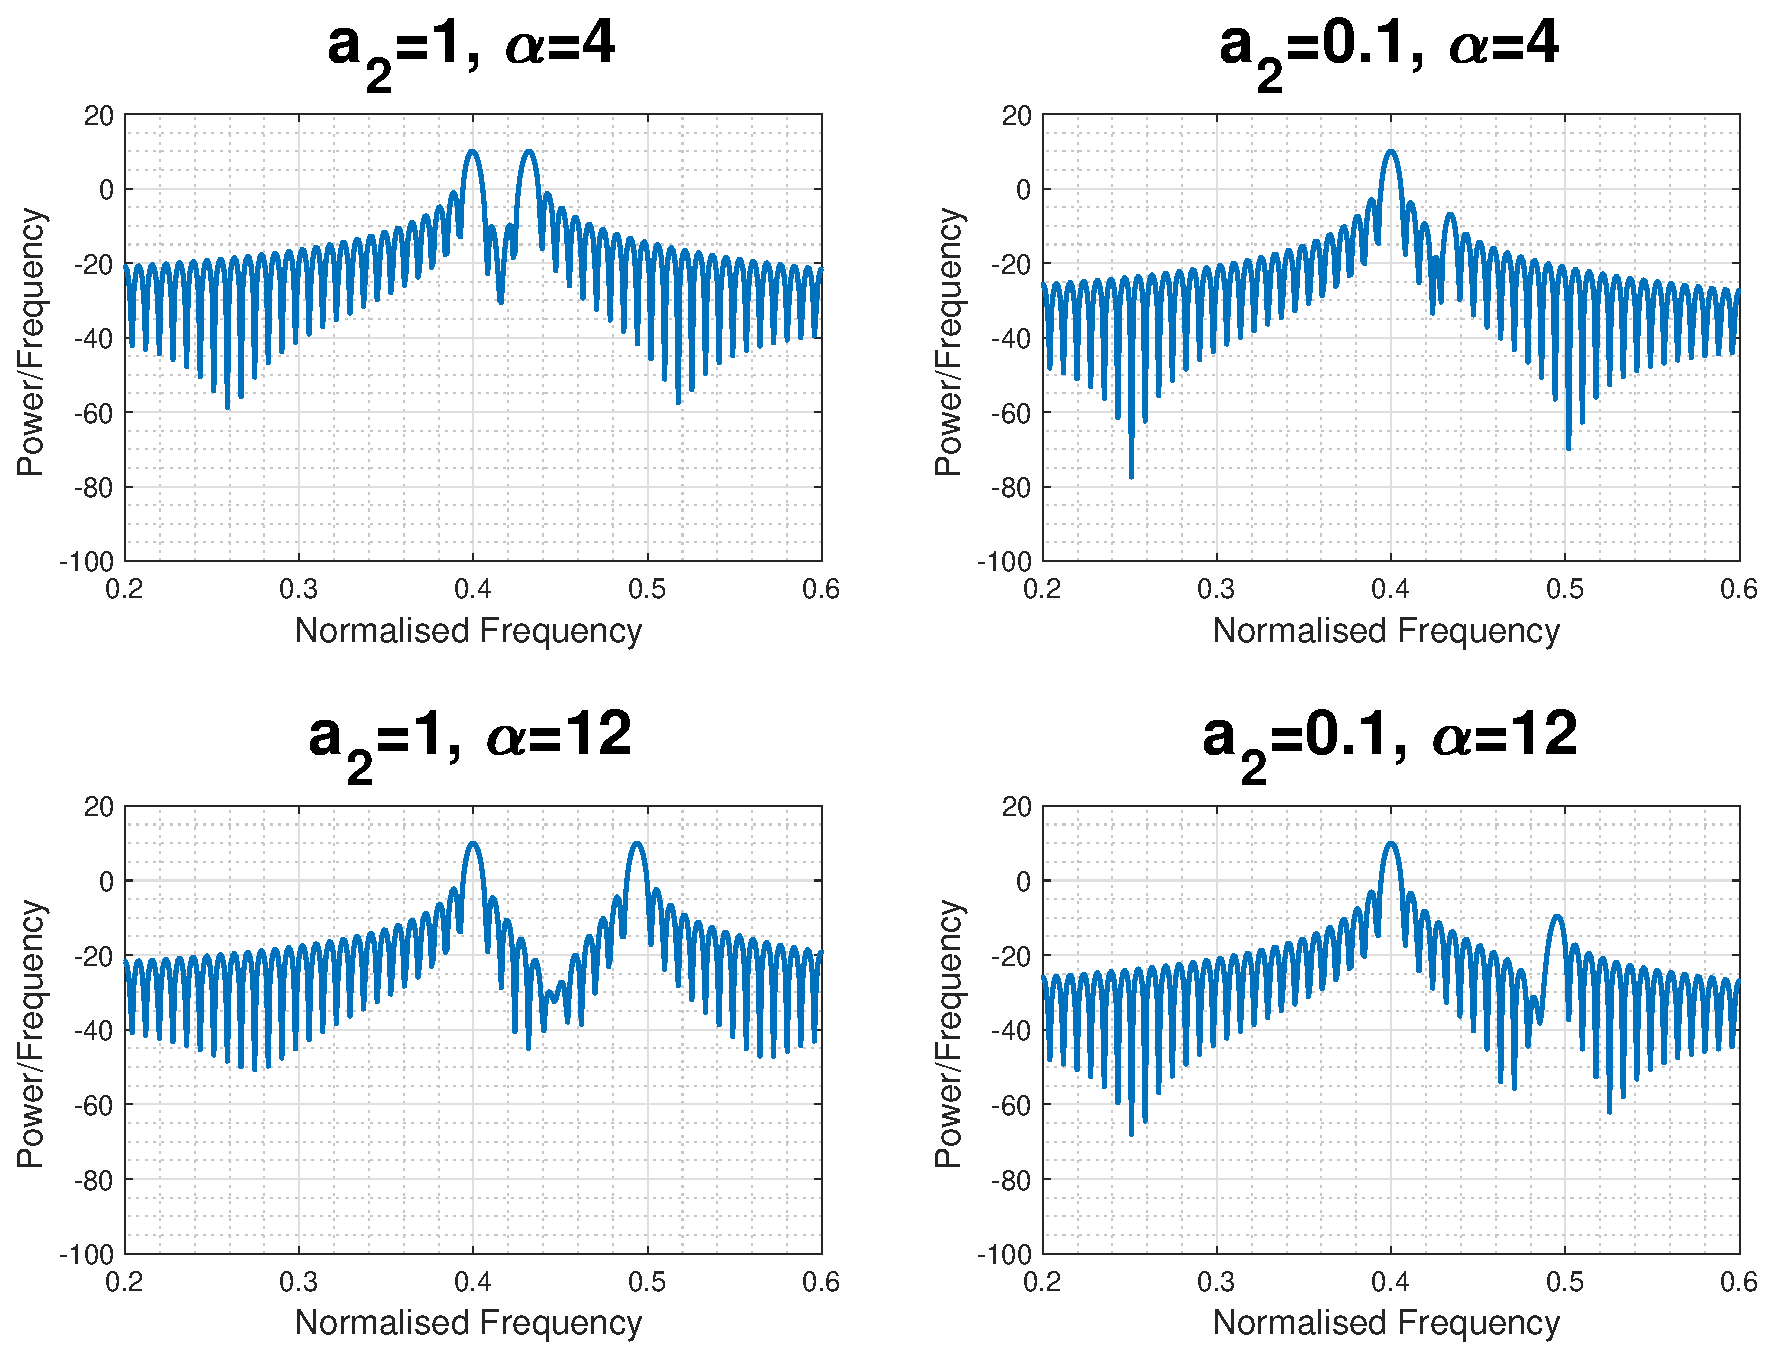
\includegraphics[width=0.49\textwidth]{part1/periodogram_leakage_bartlett_part_1}
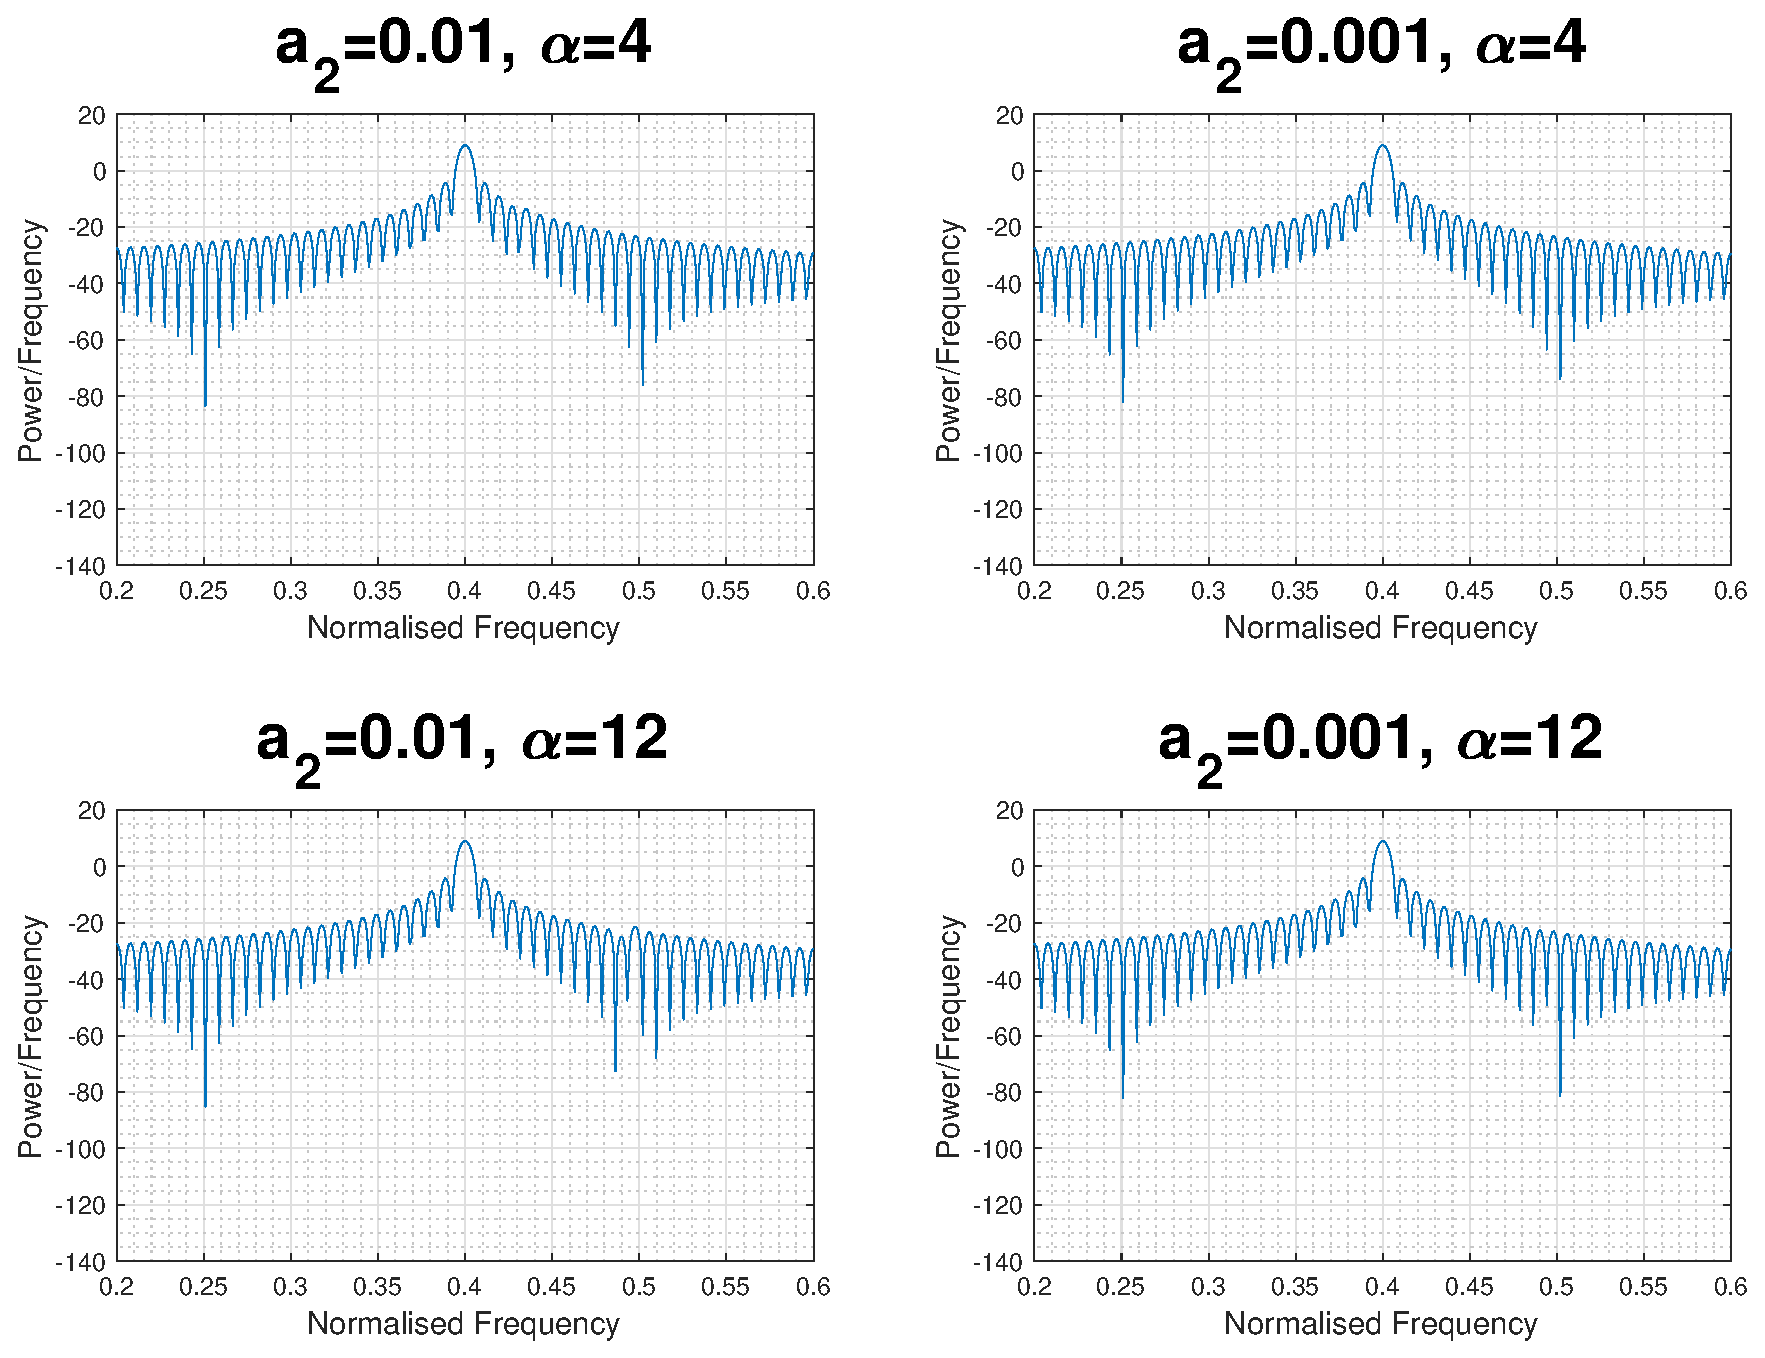
\includegraphics[width=0.49\textwidth]{part1/periodogram_leakage_bartlett_part_2}
\caption{Random Caption}
\end{figure}

\begin{figure}[H]
\centering{}
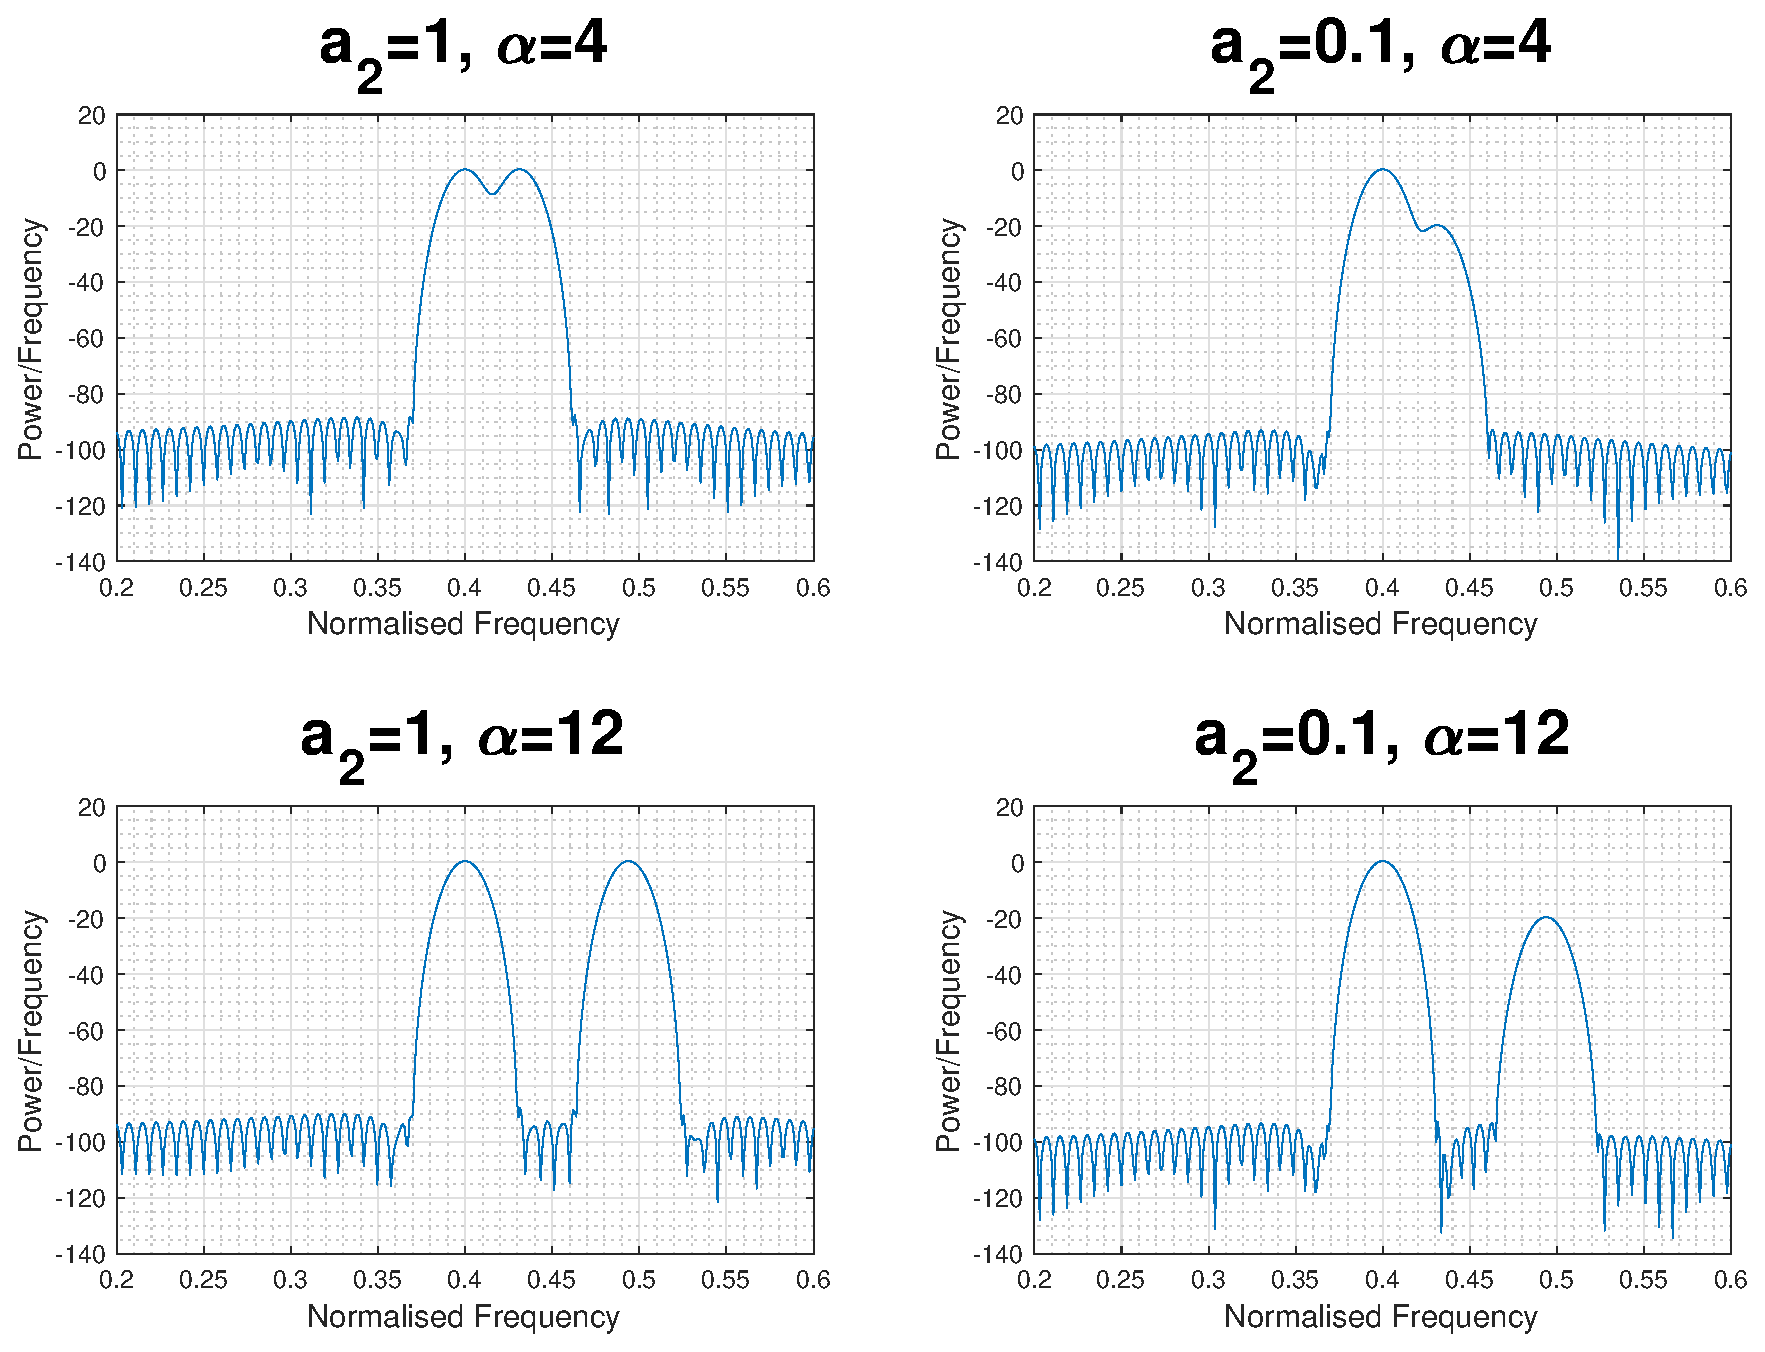
\includegraphics[width=0.49\textwidth]{part1/periodogram_leakage_chebwin_part_1}
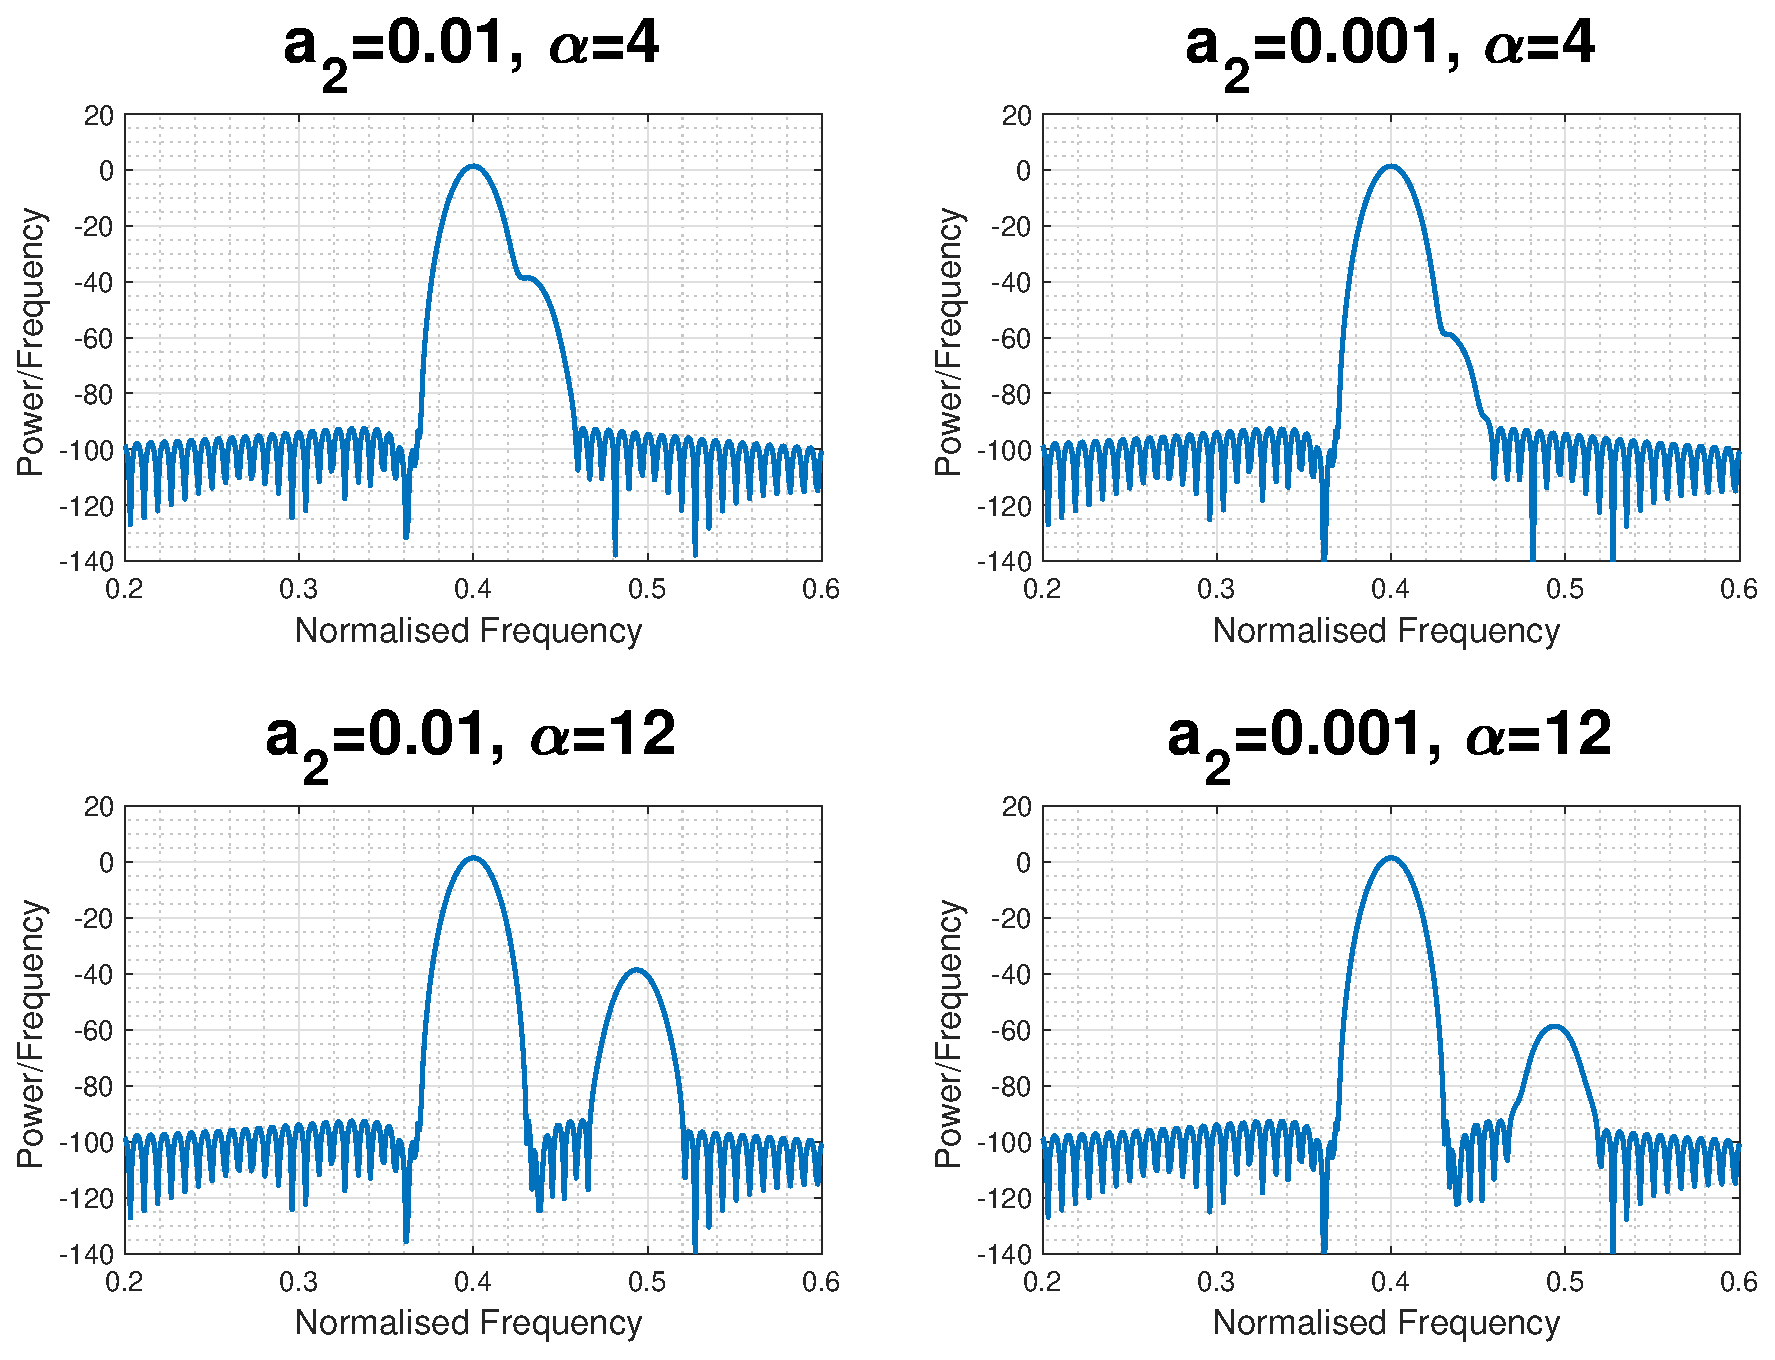
\includegraphics[width=0.49\textwidth]{part1/periodogram_leakage_chebwin_part_2}
\caption{Random Caption}
\end{figure}



